\documentclass[11pt,a4paper]{article}
% ==========================================================================
%  Shared preamble for both language editions of the Euclid's-path article.
%  Language-neutral: packages, theorem environments, notation, status macros.
%  (babel main language is set in each main file: *.en.tex / *.ru.tex.)
% ==========================================================================

\usepackage[T2A,T1]{fontenc}   % T2A also present so the Russian edition sets Cyrillic
\usepackage[utf8]{inputenc}
\usepackage[a4paper,margin=1in]{geometry}

% Map blackboard-bold letters and superscripts that occasionally slip into prose
% as literal Unicode into proper math (both editions are then robust to them).
\DeclareUnicodeCharacter{211D}{\ensuremath{\mathbb{R}}}
\DeclareUnicodeCharacter{2115}{\ensuremath{\mathbb{N}}}
\DeclareUnicodeCharacter{2124}{\ensuremath{\mathbb{Z}}}
\DeclareUnicodeCharacter{211A}{\ensuremath{\mathbb{Q}}}
\DeclareUnicodeCharacter{2102}{\ensuremath{\mathbb{C}}}
\DeclareUnicodeCharacter{00B2}{\ensuremath{^{2}}}
\DeclareUnicodeCharacter{00B3}{\ensuremath{^{3}}}

\usepackage{amsmath,amssymb,amsthm,mathtools}
\usepackage{xcolor}
\usepackage{graphicx}
\usepackage{booktabs}
\usepackage{enumitem}
\usepackage[hidelinks]{hyperref}
\usepackage{cleveref}
% make `_` print literally in text mode (Lean names like foo_bar need no escaping);
% [strings] keeps `_` safe inside \label/\ref/\cite keys. Load last so it patches the rest.
\usepackage[strings]{underscore}

% ---- theorem-head names (English defaults; the Russian edition renews them) ----
\providecommand{\nmTheorem}{Theorem}
\providecommand{\nmLemma}{Lemma}
\providecommand{\nmProposition}{Proposition}
\providecommand{\nmCorollary}{Corollary}
\providecommand{\nmDefinition}{Definition}
\providecommand{\nmConjecture}{Conjecture}
\providecommand{\nmRemark}{Remark}

% ---- theorem environments: ONE shared counter, numbered by section ----
\theoremstyle{plain}
\newtheorem{theorem}{\nmTheorem}[section]
\newtheorem{lemma}[theorem]{\nmLemma}
\newtheorem{proposition}[theorem]{\nmProposition}
\newtheorem{corollary}[theorem]{\nmCorollary}
\theoremstyle{definition}
\newtheorem{definition}[theorem]{\nmDefinition}
\newtheorem{conjecture}[theorem]{\nmConjecture}
\theoremstyle{remark}
\newtheorem*{remark}{\nmRemark}

% ---- honesty status badges (colour + textual, pdflatex-safe) ----
\newcommand{\statusdot}[1]{\textcolor{#1}{\ensuremath{\bullet}}}
\newcommand{\green}{\statusdot{green!55!black}}   % machine-proved, standard axioms
\newcommand{\yellow}{\statusdot{orange!85!black}} % AXIOM-TAINTED (conditional on the first cause)
\newcommand{\red}{\statusdot{red!75!black}}       % open node / input
\newcommand{\warn}{\statusdot{orange!60!black}}   % vacuity / caution

% ---- notation ----
\newcommand{\N}{\mathbb{N}}
\newcommand{\Z}{\mathbb{Z}}
\newcommand{\R}{\mathbb{R}}
\newcommand{\code}[1]{\texttt{#1}}                % Lean declaration name
\newcommand{\Om}{\Omega}
\DeclareMathOperator{\DescentStep}{DescentStep}
\DeclareMathOperator{\Clean}{Clean}
\DeclareMathOperator{\ActiveEdge}{ActiveEdge}
\DeclareMathOperator{\BoundaryExit}{BoundaryExit}

% the single quarantined axiom, referenced throughout
\newcommand{\axiom}{\code{step00FirstCause}}

\usepackage[english,russian]{babel}

% Russian theorem-head names (renew the English defaults from macros.tex)
\renewcommand{\nmTheorem}{Теорема}
\renewcommand{\nmLemma}{Лемма}
\renewcommand{\nmProposition}{Предложение}
\renewcommand{\nmCorollary}{Следствие}
\renewcommand{\nmDefinition}{Определение}
\renewcommand{\nmConjecture}{Гипотеза}
\renewcommand{\nmRemark}{Замечание}

\title{Вечный двигатель Евклида:\\
  машинно-проверенное прочтение великих гипотез\\
  через единственную аксиому}
\author{Д.~С.~Семёнов \and Л.~Р.~Галиева}
\date{2026}

\begin{document}
\maketitle

\begin{abstract}
Мы формализуем в системе доказательств Lean~4 программу, выстроенную вокруг одного
физического запрета: невозможности \emph{вечного двигателя} --- бесконечного спуска Ферма,
переформулированного для центров евклидовых пар $6m\pm1$. Из этого единственного факта мы
получаем машинно-проверенную редукцию гипотезы о простых-близнецах к \emph{одному} открытому
узлу и прочитываем семейство вопросов уровня проблем тысячелетия --- гипотезу Римана,
$\mathrm{P}$ против $\mathrm{NP}$, Янга--Миллса, Ходжа, Навье--Стокса,
Бёрча--Свиннертон-Дайера, а также простые Мерсенна, задачу Коллатца и арифметический
зоопарк --- как тени того же запрета на разных объектах. Узел нельзя закрыть изнутри,
поскольку его самообоснование построило бы запрещённый двигатель; поэтому он принимается
\emph{извне} единственной карантинной аксиомой --- \emph{первопричиной}. Наша главная теорема
(«высшая энергетическая несовместимость») показывает, что бесконечность близнецов нельзя ни
доказать, ни опровергнуть внутри системы без такого двигателя. Мы строго честны в том, что
доказано, а что нет: всё построение опирается \emph{ровно на одну} нестандартную аксиому и
содержит \emph{ровно один} \code{sorry} (саму гипотезу о близнецах); машинный верификатор
помечает каждую заражённую аксиомой декларацию (сейчас их $47$) и перепроверяет эти два
инварианта при каждом запуске. \textbf{Ни одна проблема тысячелетия не решена и не объявляется
решённой.} Каждое формальное утверждение статьи несёт имя соответствующей машинно-проверенной
декларации; полный исходный код Lean открыт, а идентичный контент доступен для чтения онлайн.
\end{abstract}

\begin{center}\small
\fbox{\begin{minipage}{0.92\linewidth}\centering
Машинно-проверенный исходник (Lean~4): \url{https://github.com/elamaunt/Euclids-path}\\
Тот же контент как двуязычный (русский/английский) сайт:
\url{https://elamaunt.github.io/Euclids-path/}\\[2pt]
Каждая теорема ниже называет свою Lean-декларацию; запустите
\code{lake env lean scripts/VerifyAll.lean}, чтобы перепроверить инварианты честности.
\end{minipage}}
\end{center}

\medskip
\noindent\textbf{Ключевые слова.} простые-близнецы; бесконечный спуск; формализация; Lean~4;
первопричина; гипотеза Римана; $\mathrm{P}$ против $\mathrm{NP}$; Навье--Стокс; Коллатц.

\smallskip
\noindent\textbf{MSC 2020.} 11A41, 11N05, 68V20, 03F03, 11P32.

\tableofcontents

\section{Введение}
\label{sec:intro}

Эта статья описывает одну машинно-проверенную идею и дисциплину, которая держит её честной.
Идея --- физический запрет: двигатель, который \emph{вечно} совершает нетривиальную работу
спуска, ничего при этом не теряя, существовать не может. В арифметике натуральных чисел это
метод бесконечного спуска Ферма; мы переформулируем его для центров $m$ евклидовых пар
$(6m-1,\,6m+1)$ и называем запрещённый объект \emph{вечным двигателем Евклида}. Сам запрет ---
не существует бесконечно убывающей цепи чистых евклидовых шагов --- доказан на голом ядре
Lean~4, без \code{mathlib} и без каких-либо аксиом сверх стандартных (\cref{sec:engine}).

Тезис программы состоит в том, что удивительно многие трудные вопросы суть тени этого одного
запрета, отброшенные на разные объекты. Там, где объект не может нести вечный двигатель,
структурная теорема «нет отклонения» выполняется \emph{безусловно}; открытым же остаётся всегда
одно и то же --- связь между абстрактной структурой и конкретным аналитическим объектом,
которого математика пока не предоставила. Мы проводим это прочтение через гипотезу о
простых-близнецах (стержень статьи), гипотезу Римана, $\mathrm{P}$ против $\mathrm{NP}$,
Янга--Миллса, Ходжа, Навье--Стокса, Бёрча--Свиннертон-Дайера и далее --- через простые Мерсенна,
арифметический зоопарк узоров из простых, геометрию графа спуска и задачу Коллатца.

\paragraph{Что доказано, а что нет.}
Мы настойчивы в этом пункте, потому что тема провоцирует преувеличения, а мы не хотим ни
одного. Гипотеза о простых-близнецах здесь \emph{не} доказана. Доказана же, и машинно, без
\code{sorry}, \emph{редукция}: вся близнецовая ветвь сведена к одному явному открытому узлу ---
конечному семантическому ключу, который должен разрешать определённые коллизии генеалогий
(\cref{sec:reduction}). Этот узел нельзя закрыть изнутри системы: его закрытие означало бы запуск
того самого двигателя, невозможность которого лежит в основании. Поэтому мы принимаем его
\emph{извне}, как единственную аксиому, называемую \emph{первопричиной} (\cref{sec:firstcause}),
запертую в одном карантинном модуле. Наша главная теорема, \emph{высшая энергетическая
несовместимость}, делает картину точной: бесконечность близнецов нельзя ни доказать, ни
опровергнуть внутри системы без вечного двигателя, так что конечный наблюдатель может лишь
\emph{принять} первопричину, но никогда её не вывести.

\paragraph{Дисциплина честности.}
Через всё построение проходят три цвета, и мы называем их прямо: \green{}~утверждение
машинно-доказано при стандартных аксиомах (сюда входит и \emph{зелёная условная теорема}, чьё
условие --- названный вход, а не аксиома); \yellow{}~утверждение \emph{заражено аксиомой}, то
есть зависит от первопричины; \red{}~объект действительно открыт. Отдельный верификатор обходит
каждую декларацию репозитория, собирает аксиомы, от которых она зависит, и обеспечивает два
неизменных инварианта: единственная нестандартная аксиома во всём построении --- \axiom{}, а
единственное заражённое \code{sorry} утверждение --- сама гипотеза о близнецах. На момент письма
верификатор сообщает ровно одну нестандартную аксиому, ровно один \code{sorry} и $47$
заражённых аксиомой деклараций; зелёный модуль подделать нельзя, а аксиом-трекер не оставляет
декрету места спрятаться за зелёной вывеской. Четырежды в ходе работы внутренний аудит находил
пустую обёртку раньше, чем она попадала в витрину (мы отмечаем эти вакуумности там, где они
возникли); то, что они пойманы машиной, --- лучший довод доверять частям, прошедшим витрину.

\paragraph{Воспроизводимость.}
Всё в этой статье --- отражение исходного кода Lean~4~\cite{lean4,mathlib,euclidspath-repo}.
Каждое формальное утверждение ниже помечено именем своей машинно-проверенной декларации,
набранным \code{машинописью}. Полный исходный код открыт по адресу
\url{https://github.com/elamaunt/Euclids-path}; идентичный контент доступен как двуязычный сайт
по адресу \url{https://elamaunt.github.io/Euclids-path/}. Сборка командой \code{lake build}
проверяет всё построение, а \code{lake env lean scripts/VerifyAll.lean} заново устанавливает два
инварианта честности и громко падает, если нарушен любой из них.

\paragraph{План.}
\cref{sec:engine} доказывает невозможность двигателя и его необратимость. \cref{sec:carrier}
фиксирует носитель двойки и законы сохранения, делающие пары «разделёнными». \cref{sec:reduction}
сводит гипотезу о близнецах к одному узлу. \cref{sec:firstcause} вводит первопричину и доказывает
главную теорему. \cref{sec:riemann,sec:pnp,sec:ymhodge,sec:ns} прочитывают гипотезу Римана,
$\mathrm{P}$ против $\mathrm{NP}$, Янга--Миллса и Ходжа, а также Навье--Стокса через двигатель.
\cref{sec:zoo,sec:geometry,sec:bsd} разбирают ветвь Мерсенна и арифметический зоопарк, геометрию
пути и Бёрча--Свиннертон-Дайера вместе с несколькими открытыми соседями. \cref{sec:collatz}
разбирает задачу Коллатца, включая декрет, который был взят и затем снят, когда его закон был
машинно опровергнут. \cref{sec:coda} --- синтез; \cref{sec:status} даёт честный глобальный статус
и процедуру верификации; \cref{sec:figures} задаёт алгоритм генерации каждого рисунка.

\section{Двигатель Евклида: невозможность вечного спуска}\label{sec:engine}

Программа сводит гипотезу о простых-близнецах к поведению одного динамического объекта --- цепи
самоподобных евклидовых уравнений, которую мы называем \emph{двигателем Евклида}, --- и опирает всё
здание на единственный факт: двигатель не может работать вечно. Предположим, что близнецов лишь
конечное число. Тогда, начиная с некоторого масштаба, каждая пара $(6m-1,\,6m+1)$ содержит составную
сторону, разложение которой обнажает активный делитель; его удаление порождает структурно такое же
евклидово уравнение строго меньшего центра. Повторяя, получаем бесконечную цепь чистых спусков, ни
на одном шаге не выходящую из clean-ядра, --- вечно работающий двигатель, совершающий нетривиальную
работу спуска и ничего при этом не теряющий. Мы доказываем, что такого двигателя не существует. Это
бесконечный спуск Ферма, переформулированный для центров евклидовых пар: состояние описывается одним
натуральным числом --- его \emph{высотой}, --- а один успешный шаг уменьшает высоту строго и
\emph{мультипликативно}, после чего работает лишь арифметика $\N$. Всё нижеследующее проверено машинно
на голом ядре Lean~4, без \code{mathlib} (\code{EuclidsPath/Engine/EPMI.lean},
\code{EuclidsPath/Engine/Irreversibility.lean}, \code{EuclidsPath/Engine/UniversalEngine.lean})~\cite{lean4,euclidspath-repo}.

\subsection{Шаг спуска и его строгость}

Абстрагируемся от арифметической начинки и оставим лишь то, что нужно для доказательства
невозможности. Состояние несёт единственную числовую характеристику --- высоту $h\in\N$,
содержательно центр $m$ пары $(6m-1,\,6m+1)$.

\begin{definition}[\code{DescentStep}]\label{thm:DescentStep}
Пусть $A\in\N$ --- фиксированный масштабный порог (нижняя граница активных множителей). Один успешный
clean-спуск с высоты $h$ на высоту $h'$ есть отношение
\begin{equation}\label{eq:descentstep}
  \mathrm{DescentStep}\,A\,h\,h' \;:=\; A\cdot h' < h.
\end{equation}
\end{definition}

Шаг фиксирует не абы какое, а \emph{мультипликативное} убывание: новая высота меньше в $A$ раз (с
точностью до строгости). Именно множитель $A$, а не разность, задаёт скорость спуска и делает
конечность неизбежной.

\begin{lemma}[\code{descent_strict}]\label{thm:descent_strict}
\green{}\; Если $1\le A$ и $\mathrm{DescentStep}\,A\,h\,h'$, то $h'<h$.
\end{lemma}

\emph{Идея доказательства.} Из $1\le A$ следует $h'\le A\cdot h'$ (умножение на положительный
множитель не уменьшает), а $A\cdot h'<h$ --- по \cref{eq:descentstep}; транзитивность даёт $h'<h$.
Лемма отделяет \emph{направление} спуска (высота падает) от его \emph{скорости} (падает в $A$ раз).

\subsection{Невозможность бесконечного спуска}

\begin{theorem}[\code{no_infinite_descent}]\label{thm:no_infinite_descent}
\green{}\; Пусть $1\le A$. Не существует последовательности высот $H:\N\to\N$, для которой каждый шаг
был бы успешным $A$-спуском, то есть
\begin{equation}\label{eq:perpetualheights}
  \forall\, t,\quad \mathrm{DescentStep}\,A\,(H\,t)\,(H\,(t+1)).
\end{equation}
Из существования такой последовательности выводится \code{False}.
\end{theorem}

\begin{proof}
Рассмотрим величину $H\,t+t$. На каждом шаге высота падает как минимум на $1$ (\cref{thm:descent_strict}),
а счётчик $t$ растёт на $1$; значит $H\,t+t$ не возрастает, и по индукции $\forall\,t,\ H\,t+t\le H\,0$.
Подставив $t=H\,0+1$, получаем $H\,(H\,0+1)+(H\,0+1)\le H\,0$, левая часть которого уже превосходит
$H\,0$ --- противоречие. В Lean индукция закрывается тактикой \code{omega}; \code{\#print axioms}
подтверждает, что теорема не зависит ни от каких аксиом и свободна от \code{sorry}.
\end{proof}

Мультипликативное убывание $H_t<H_0/A^{t}$ уводит высоту ниже $1$ за конечное число шагов, а
положительное целое не может быть меньше $1$: натуральный ряд имеет дно, и дискретный спуск обязан его
достичь. Для самого противоречия достаточно $A=1$ (порядковая полнота $\N$); множитель $A\ge 1$ даёт
количественную скорость. Это сильнее физического второго закона: поскольку высота --- целое со строгим
дном, спуск не просто затухает асимптотически, а останавливается не более чем за $H\,0$ шагов
(\cref{thm:turned_engine_halts}).

\subsection{Структурная форма: состояние и boundary-exit}

Чтобы связать абстрактную теорему с содержательной картиной, введём явное состояние и оператор шага,
различающий два исхода удаления активного множителя.

\begin{definition}[\code{State}]\label{thm:State}
Состояние двигателя есть структура с единственным полем $\mathrm{height}:\N$; содержательно это центр
$m$ текущей евклидовой пары. Шаг над состоянием $s$ --- индуктивный тип с двумя конструкторами,
\begin{equation}\label{eq:step}
  \mathrm{Step}\,A\,s \;=\;
  \begin{cases}
    \texttt{clean}\ s'\ (A\cdot s'.\mathrm{height} < s.\mathrm{height}), & \text{успешный спуск в clean-состояние,}\\[2pt]
    \texttt{boundary}, & \text{поглощающий выход } \bot,
  \end{cases}
\end{equation}
где ветвь \texttt{clean} несёт свидетельство мультипликативного убывания, а \texttt{boundary}
фиксирует выход из clean-ядра на границу, откуда нет возврата.
\end{definition}

\begin{theorem}[\code{no_perpetual_engine}]\label{thm:no_perpetual_engine}
\green{}\; Пусть $1\le A$. Нет траектории $\mathrm{run}:\N\to\mathrm{State}$, в которой каждый шаг ---
успешный clean-спуск, то есть
$A\cdot(\mathrm{run}\,(t+1)).\mathrm{height} < (\mathrm{run}\,t).\mathrm{height}$ для всех $t$.
\end{theorem}

\emph{Идея доказательства.} Приведение к абстрактной форме: берём высоты
$t\mapsto(\mathrm{run}\,t).\mathrm{height}$ и применяем \cref{thm:no_infinite_descent}. Это и есть
«нет вечного двигателя Евклида».

\begin{theorem}[\code{boundary_dichotomy}]\label{thm:boundary_dichotomy}
\green{}\; Для любого шага $st:\mathrm{Step}\,A\,s$ выполнено ровно одно из двух:
\begin{equation}\label{eq:dichotomy}
  \bigl(\exists\, s'\,h,\ st = \texttt{clean}\ s'\ h\bigr)\ \lor\ \bigl(st = \texttt{boundary}\bigr).
\end{equation}
\end{theorem}

\emph{Идея доказательства.} Разбор случаев по конструкторам \cref{eq:step}. Это типовая фиксация
boundary-exit law: descended-центр либо остаётся clean (высота строго упала в $A$ раз), либо выходит
на поглощающую границу $\bot$, откуда нет clean-продолжения той же ветви. Граница поглощает:
$\bot\not\to S$.

\subsection{Необратимость и стрела времени}

\cref{thm:no_infinite_descent} отвечает на вопрос «всегда ли двигатель останавливается?». Соседний
модуль \code{Irreversibility.lean} закрывает «может ли он повернуть назад?», давая дискретный аналог
второго закона термодинамики. Всё это доказано машинно только на стандартных аксиомах, без обращения
к распределению простых.

\begin{theorem}[\code{engine_never_returns}]\label{thm:engine_never_returns}
\green{}\; Пусть $1\le A$ и $H:\N\to\N$ удовлетворяет \cref{eq:perpetualheights}. Тогда $H$ строго
антимонотонна:
\begin{equation}\label{eq:strictanti}
  \mathrm{StrictAnti}\,H \;:\Longleftrightarrow\; \bigl(\forall\, s\,t,\; s<t \Rightarrow H\,t<H\,s\bigr).
\end{equation}
\end{theorem}

\emph{Идея доказательства.} Локальное строгое убывание $H(n+1)<H(n)$ из \cref{thm:descent_strict}
поднимается до глобальной антимонотонности через \code{strictAnti_nat_of_succ_lt}: на $\N$ убывание
на каждом единичном шаге эквивалентно убыванию на любом интервале. Высота есть координата
термодинамического времени, а \cref{eq:strictanti} --- формальная стрела времени: двигатель, тронувшись
в спуск, не может восстановить прежнее состояние. Это описывает любую цепь успешных спусков, \emph{буде
такая дана}; может ли она быть бесконечной --- отрицательно решает \cref{thm:no_infinite_descent}.

\begin{theorem}[\code{fuel_ascent_strictMono}]\label{thm:fuel_ascent_strictMono}
\green{}\; Отображение $n\mapsto n+1$ строго монотонно: $\mathrm{StrictMono}\,(\lambda n.\,n+1)$.
\end{theorem}

\emph{Идея доказательства.} Тривиально $n<n+1$. Тривиальность формы скрывает содержание: successor-цепь
$0,1,2,\dots$ --- бесконечная строго возрастающая траектория. Прибавление $+1$ --- «топливо»: бо́льших
центров всегда хватает. Сопоставление с \cref{thm:no_infinite_descent} обнажает асимметрию
термодинамической оси --- вверх бесконечно, вниз конечно. Эта асимметрия и есть стрела.

\begin{theorem}[\code{turned_engine_halts}]\label{thm:turned_engine_halts}
\green{}\; Пусть $H:\N\to\N$ и двигатель сделал $k$ строгих шагов вниз, то есть $H(t+1)<H(t)$ для всех
$t<k$. Тогда
\begin{equation}\label{eq:haltbound}
  k \;\le\; H(0).
\end{equation}
\end{theorem}

\emph{Идея доказательства.} Индукцией доказывается инвариант $H(t)+t\le H(0)$ для всех $t\le k$;
подстановка $t=k$ и отбрасывание $H(k)\ge 0$ дают \cref{eq:haltbound}. Это тот же баланс «высота плюс
время не растёт», что и в \cref{thm:no_infinite_descent}, прочитанный как конечная оценка, а не как
выход на противоречие: любой поворот вниз --- конечный путь длиной не более начальной высоты.

\subsection{Универсальная форма: двигатель против фундированности}

Невозможность выше есть тень единственного порядково-теоретического факта, формализованного в
\code{UniversalEngine.lean} над произвольным отношением. Это чтение несёт вся статья: где носитель
фундирован, двигатель запрещён \emph{безусловно}; где нет --- двигатель работает.

\begin{definition}[\code{PerpetualEngine}]\label{thm:PerpetualEngine}
Для отношения $r$ на типе $\alpha$ вечный двигатель есть бесконечная строго $r$-убывающая цепь:
\begin{equation}\label{eq:perpetualengine}
  \mathrm{PerpetualEngine}\,r \;:=\; \exists\, f:\N\to\alpha,\ \forall\, n,\ r\,(f(n+1))\,(f\,n).
\end{equation}
\end{definition}

\begin{theorem}[\code{perpetualEngine_iff_not_wellFounded}]\label{thm:perpetualEngine_iff_not_wellFounded}
\green{}\; Для любого $r$ на $\alpha$
\begin{equation}\label{eq:dividingline}
  \mathrm{PerpetualEngine}\,r \;\Longleftrightarrow\; \neg\,\mathrm{WellFounded}\,r.
\end{equation}
\end{theorem}

\emph{Идея доказательства.} Разворачивая $\mathrm{WellFounded}$ через характеризацию убывающими цепями,
двигатель \cref{eq:perpetualengine} есть буквально убывающая цепь, отсутствие которой и есть
фундированность. Это точная разделяющая линия: двигатель и фундированность взаимно дополнительны.

\begin{theorem}[\code{no_perpetual_engine_of_wellFounded}]\label{thm:no_perpetual_engine_of_wellFounded}
\green{}\; Если $\mathrm{WellFounded}\,r$, то $\neg\,\mathrm{PerpetualEngine}\,r$.
\end{theorem}

\emph{Идея доказательства.} Немедленно из \cref{thm:perpetualEngine_iff_not_wellFounded}. Невозможность
внутренняя, почти определительная: собственная определяющая цепь двигателя есть ровно то, что запрещает
фундированность. \cref{thm:no_infinite_descent} --- частный случай $r={<}$ на $\N$
(\code{no_perpetual_engine_on_nat}), с высотой в роли ранга.

\begin{theorem}[\code{no_perpetual_engine_of_rank}]\label{thm:no_perpetual_engine_of_rank}
\green{}\; Пусть $\rho:\alpha\to\beta$ с фундированным $(\beta,s)$, и каждый $r$-шаг строго уменьшает
ранг: $\forall\, x\,y,\ r\,x\,y \Rightarrow s\,(\rho\,x)\,(\rho\,y)$. Тогда
$\neg\,\mathrm{PerpetualEngine}\,r$.
\end{theorem}

\emph{Идея доказательства.} Двигатель $f$ для $r$ переносился бы вдоль $\rho$ в убывающую цепь
$\rho\circ f$ в фундированном $(\beta,s)$, противореча \cref{thm:no_perpetual_engine_of_wellFounded}.
$\N$-ранговая специализация (\code{no_perpetual_engine_of_natRank}) есть унификация: всякий фронт спуска
программы --- следствие этой одной теоремы, получаемое предъявлением ранга, строго убывающего вдоль
шагов.

\begin{theorem}[\code{perpetualEngine_on_real}]\label{thm:perpetualEngine_on_real}
\green{}\; На континууме двигатель работает: $\mathrm{PerpetualEngine}\,(<)$ на $\R$.
\end{theorem}

\emph{Идея доказательства.} Свидетель $(1/2)^n$ --- бесконечная строго $(<)$-убывающая цепь в $\R$;
значит, по \cref{thm:perpetualEngine_iff_not_wellFounded}, строгий порядок на $\R$ не фундирован. Это
честная граница контроллёра: на дискретных носителях двигатель запрещён и спуск обрывается, а на
вещественных вечный спуск реализуется. Запрет живёт в дискретности, а не в анализе.

\medskip

Мы ввели центральный объект и доказали, машинно и без аксиом, что бесконечно он работать не может
(\cref{thm:no_infinite_descent,thm:no_perpetual_engine}), не поворачивает назад
(\cref{thm:engine_never_returns}) и, свернув вниз, останавливается за конечное число шагов
(\cref{thm:turned_engine_halts}); дихотомия (\cref{thm:boundary_dichotomy}) оставляет поглощающую
границу единственной альтернативой продолжению. Честно очертим границу доказанного: это невозможность
бесконечного \emph{локального} clean-спуска вдоль одной ветви. Глобальный результат о непокрытии отсюда
\emph{не следует} автоматически --- мыслимо конечное дерево ограниченной глубины, каждая ветвь которого
честно обрывается absorbing boundary-leaf и которое при этом покрывает все центры. План закрытия
поднимает запрет с ветви на всё дерево, переоформленный как multi-rank non-cover с редукцией ранга к
rank-$1$ обструкции соседа; этот единственный открытый узел разбирается в \cref{sec:reduction}.
Двигатель же поставляет локальный закон конечности, на котором стоит вся редукция.

\section{Носитель двойки и законы сохранения}\label{sec:carrier}

Прежде чем спускаться по цепи звеньев двигателя, нужно выделить то, что евклидов шаг
\emph{сохраняет}, и то, что \emph{разделяет} две стороны пары. Настоящий раздел фиксирует и то и
другое: двойка есть общий делитель, удерживающий стороны врозь, и одновременно инвариант, который
переносит спуск. Всё здесь элементарно --- делимость и кольцевая арифметика на чистом ядре
Lean~4 и \code{mathlib}~\cite{lean4,mathlib}, без анализа, распределения и сита --- и всякое
утверждение ниже \green{}~машинно доказано при стандартных аксиомах, кроме единственного открытого
узла в конце.

Всюду мы работаем с \emph{центром} $m\ge 1$ евклидовой пары, чьи \emph{стороны} суть кандидаты
$6m-1$ и $6m+1$; всякое простое $p>3$ лежит в классе $\pm1\pmod 6$, так что пара с разностью $2$
выше $3$ центрируется в кратном шести. Условие $1\le m$ делает $6m-1$ честным предшественником $6m$
в $\N$ (усечённое вычитание), так что $6m+1=(6m-1)+2$ есть равенство натуральных чисел.

\subsection{Носитель двойки}

\begin{definition}[общий делитель сторон]\label{def:shared-divisor}
Натуральное $p$ есть \emph{общий делитель сторон} центра $m$, если одновременно $p\mid(6m-1)$ и
$p\mid(6m+1)$.
\end{definition}

Стороны отстоят ровно на два, $(6m+1)-(6m-1)=2$, и эта фиксированная разность управляет всей их
совместной делимостью.

\begin{theorem}[\code{twin\_sides\_shared\_dvd\_two}]\label{thm:twin_sides_shared_dvd_two}
\green{} Пусть $m\ge 1$ и $p\mid(6m+1)$, $p\mid(6m-1)$. Тогда $p\mid 2$.
\end{theorem}

\emph{Идея доказательства.} Перепишем б\'{о}льшую сторону через меньшую, $6m+1=(6m-1)+2$ (закрывается
\code{omega} над $\N$ при $m\ge1$). Тогда $p\mid\bigl((6m-1)+2\bigr)$, и так как $p\mid(6m-1)$,
свойство делимости суммы с делимым слагаемым (\code{Nat.dvd\_add\_right}) вынуждает $p\mid 2$.
Работает только \emph{разность} сторон: по существу это утверждение $\gcd(6m-1,\,6m+1)\mid 2$.

Так как у двойки лишь делители $1$ и $2$, ни одно простое выше двух не может занять обе стороны
сразу.

\begin{theorem}[\code{no\_large\_shared\_divisor}]\label{thm:no_large_shared_divisor}
\green{} Пусть $m\ge 1$ и $p>2$. Тогда $p\mid(6m+1)$ и $p\mid(6m-1)$ не могут выполняться
одновременно.
\end{theorem}

\emph{Идея доказательства.} По \cref{thm:twin_sides_shared_dvd_two} $p\mid 2$, откуда $p\le 2$ по
оценке делителя (\code{Nat.le\_of\_dvd}, положительность через \code{decide}); это противоречит
$2<p$ (\code{omega}). Это \emph{эксклюзивность}: простое $p>2$ делит не более одной стороны. Обе
теоремы \srcpath{Engine/Carrier.lean} доказаны в чистом ядре Lean~4, без \code{mathlib}, на трёх
примитивах. Эксклюзивность позволяет считать шесть активных множителей rank-$(3,3)$ разложения
различными и служит арифметическим источником отрицательной ассоциации в
\cref{thm:exclusive_no_backward}. Двойка --- это \emph{носитель}: она разделяет стороны наверху и
переносится вниз, сохраняющаяся величина, двойственная строго убывающей высоте из
\cref{sec:engine}.

\subsection{Первый закон: сохранение двойки}

При переходе к \emph{мультипликативным} координатам --- разложении сторон в произведения активных
простых слоя $(A,A^2]$ --- разделяющая двойка не размывается, а проступает как \emph{детерминант}
линейной системы, связывающей множители. Детерминант нельзя подвинуть: он равен $2$ (или
фиксированному кратному), либо решения нет. Получающееся семейство тождеств мы называем
\emph{первым законом}; во всех координатах оно имеет вид $XY-ZW=2K$, базовый случай $K=1$ даёт
$XY-ZW=2$. Термин ``закон'' употреблён в физическом смысле сохраняющегося заряда, а не логической
аксиомы.

\begin{definition}[rank-$(3,3)$ центр]\label{def:rank33}
Центр $m$ есть \emph{rank-$(3,3)$}, если существуют натуральные $a\le b\le v$ и $q\le r\le s$ с
\begin{equation}\label{eq:rank33}
6m-1=abv,\qquad 6m+1=qrs.
\end{equation}
\end{definition}

\begin{theorem}[\code{det\_law\_rank33}]\label{thm:det_law_rank33}
\green{} Пусть $1\le m$, $6m-1=abv$ и $6m+1=qrs$. Тогда $qrs=abv+2$.
\end{theorem}

\emph{Идея доказательства.} Разность $qrs-abv$ равна разности сторон $(6m+1)-(6m-1)=2$, но теперь
выражена через множители, а не через $m$; в Lean система линейно влечёт $qrs=abv+2$ (\code{omega},
с $1\le m$, снимающим неоднозначность усечённого вычитания). Это первая жёсткость: пять из шести
множителей $a,b,v,q,r,s$ определяют шестой. Мы фиксируем лишь жёсткость --- мы \emph{не} считаем
rank-$(3,3)$ центры и никогда не выдаём одно за другое.

Свёртка по одному множителю с каждой стороны в продукт-переменную превращает двойку в буквальный
детерминант $2\times2$.

\begin{definition}[продукт-координаты]\label{def:product-coords}
Для rank-$(3,3)$ центра положим $C=av$ и $D=qs$, так что стороны суть $Cb=6m-1$ и $Dr=6m+1$ со
свободными множителями $b,r$.
\end{definition}

\begin{theorem}[\code{det\_law\_CD}]\label{thm:det_law_CD}
\green{} Над $\Z$: если $Cb=6m-1$ и $Dr=6m+1$, то
\begin{equation}\label{eq:detCD}
Cb-Dr=-2.
\end{equation}
\end{theorem}

\emph{Идея доказательства.} Вычитание гипотез: $Cb-Dr=(6m-1)-(6m+1)=-2$ (\code{linear\_combination
h1 - h2}). Знак $-2$ --- ориентированный детерминант строк $(C,-D)$ против $(b,r)^\top$. При
$\gcd(C,D)=1$ \cref{eq:detCD} редуцируется по модулю $D$ к $b\equiv-2\,\overline{C}\pmod D$:
свободный множитель $b$ лежит в \emph{одном} классе вычетов по модулю $D=qs$. Это ``zero-one slot''
за верхними оценками счёта --- если $b$ загнан в интервал короче $D$, в фиксированном боксе
$(a,v,q,s)$ допустимо не более одного $b$. Мы фиксируем алгебраическую жёсткость; переход от неё к
счёту центров --- отдельный, аналитически тяжёлый шаг.

Первый закон --- про сохранение \emph{при движении}. Вдоль луча спуска двойка переносится с точки
на точку контролируемо.

\begin{definition}[луч и его шаг]\label{def:ray}
\emph{Лучом} назовём семейство точек с общими $v,s$, где $i$-я удовлетворяет rank-one уравнению
$u_i v+2=r_i s$, а переход задан целым шагом $u_2-u_1=sK$.
\end{definition}

\begin{theorem}[\code{det\_collapse}]\label{thm:det_collapse}
\green{} Пусть $u_1 v+2=r_1 s$, $u_2 v+2=r_2 s$, $u_2-u_1=sK$ и $s\ne 0$. Тогда
\begin{equation}\label{eq:detcollapse}
u_2 r_1-u_1 r_2=2K.
\end{equation}
\end{theorem}

\emph{Идея доказательства.} Домножим цель на $s$ и подставим оба rank-one уравнения:
$s(u_2 r_1-u_1 r_2)=u_2(u_1 v+2)-u_1(u_2 v+2)=2(u_2-u_1)=2sK$; слагаемые с $v$ сокращаются --- вот
где двойка выживает --- а \code{mul\_left\_cancel\char`_0\ hs} снимает $s\ne 0$. Название точно:
$u_i,r_i$ могут расти, но их перекрёстный детерминант схлопывается к строго линейной по $K$
функции с коэффициентом $2$. Спуск --- это шаг $K=1$, несущий ровно одну двойку.

Спуск по природе \emph{квадратичен}: евклидово деление сравнивает сторону с квадратом масштаба.
Следующее тождество --- диагональное ядро самоподобия.

\begin{definition}[евклидово разложение шага]\label{def:euclid-decomp}
При $abv+2=qP$ разложим $P=v^2+\Delta$ и $ab=qv+\Xi$ по масштабу $v$; остатки $\Delta,\Xi$ суть
\emph{евклидовы остатки} шага.
\end{definition}

\begin{theorem}[\code{euclid\_descent\_identity}]\label{thm:euclid_descent_identity}
\green{} При $abv+2=qP$, $P=v^2+\Delta$ и $ab=qv+\Xi$ выполнено
\begin{equation}\label{eq:euclid-descent}
q\,\Delta-v\,\Xi=2.
\end{equation}
\end{theorem}

\emph{Идея доказательства.} Раскрытие $qP=qv^2+q\Delta$ и $abv=qv^2+\Xi v$ сокращает $qv^2$,
оставляя $\Xi v+2=q\Delta$ (\code{linear\_combination -h1 - q*h2 + v*h3}). Это диагональное ядро
самоподобного спуска: после одного евклидова шага двойка воспроизводится на меньшей паре
$(\Delta,\Xi)$, так что спуск отображает ``двойку на $(a,b,v,q)$'' в тождественную меньшую задачу
``двойку на $(\Delta,\Xi)$''. Ни в одной форме правая двойка не обращается в ноль нетривиально ---
это противоречило бы $\gcd\mid 2$ и означало бы совпадение сторон; эта невозможность --
алгебраический предшественник необратимости.

Вырожденный, но полезный случай: один атом $a$ появляется дважды и две точки связаны через общий
мост $qs$. Здесь двойка переносится как масштабированная тень $12h=6\cdot 2h$, где шестёрка --- от
шага центровой решётки.

\begin{definition}[bridge-уравнение и его сдвиг]\label{def:bridge}
Повторный атом $a$ связывает две точки уравнениями $a B_1=qs\,Q_1-2$ и $a B_2=qs\,Q_2-2$ со сдвигом
$B_2-B_1=6\,(qs)\,h$.
\end{definition}

\begin{theorem}[\code{small\_det\_collapse}]\label{thm:small_det_collapse}
\green{} При $a\ne 0$, $qs\ne 0$ и указанных bridge-уравнениях
\begin{equation}\label{eq:smalldet}
B_2 Q_1-B_1 Q_2=12\,h.
\end{equation}
\end{theorem}

\emph{Идея доказательства.} Два сокращения. Сначала $qs(Q_2-Q_1)=qs\cdot 6ah$ даёт сопряжённый сдвиг
$Q_2-Q_1=6ah$ (сокращение на $qs\ne 0$). Затем
$a(B_2 Q_1-B_1 Q_2)=Q_1(aB_2)-Q_2(aB_1)+2(Q_2-Q_1)=a\cdot12h$, и сокращение на $a\ne 0$ даёт
\cref{eq:smalldet}. Двойка из моста и шестёрка из решётки перемножаются в $12$; условия ненулевости
--- содержательное требование \emph{активности} атома и моста. Собрав
\cref{thm:det_law_rank33,thm:det_law_CD,thm:det_collapse,thm:euclid_descent_identity,%
thm:small_det_collapse}, видим один скелет $XY-ZW=2K$: двойка не создаётся и не уничтожается
двигателем, а лишь переносится. Все доказаны без \code{sorry}; первый закон \emph{не} содержит
никакого счётного или распределительного утверждения.

\subsection{Спуск и граничный закон}

Пусть центр $m$ лежит в чистом ядре $\Om_A$ (обе стороны из простых $>A$) и одна сторона составна в
слое, неся активный множитель $a>A$:
\begin{equation}\label{eq:descent-step}
6m+\sigma=a\,(6n+\varepsilon),\qquad a>A,\ \varepsilon\in\{-1,+1\}.
\end{equation}
Удаляя $a$, спущенным центром объявляем то $n$ со стороной-остатком $6n+\varepsilon$. Так как $a>A$,
высота строго падает: $n<m/A$ --- поэлементная арифметика делимости, не оценка в среднем, и именно
она обрывает спуск ($m/A^t<1$ в конце концов). Введём $U:=6n+\varepsilon$.

\begin{theorem}[\code{two\_carry\_opposite}]\label{thm:two_carry_opposite}
\green{} Если $U=6n+\varepsilon$, то
\begin{equation}\label{eq:two-carry}
6n-\varepsilon=U-2\varepsilon.
\end{equation}
\end{theorem}

\emph{Идея доказательства.} $6n-\varepsilon=(6n+\varepsilon)-2\varepsilon=U-2\varepsilon$
(\code{linear\_combination -hU}). Зазор $2$ инвариантен при спуске: активный множитель $a$ унесён
из стороны-произведения, а разделяющая двойка перекочевала на противоположную сторону
$U-2\varepsilon$. То, что удерживает стороны врозь наверху ($\gcd\mid 2$), --- ровно то, что
переносится вниз.

Сторона-произведение $U=b\cdot v$ наследует множители $b,v>A$ из родословной $6m+\sigma$, так что
никакой старый малый простой её не портит.

\begin{theorem}[\code{no\_small\_divisor}]\label{thm:no_small_divisor}
\green{} Пусть $b,v$ --- простые с $A<b$, $A<v$, и $p$ --- простое с $p\le A$. Тогда
$p\nmid(b\cdot v)$.
\end{theorem}

\emph{Идея доказательства.} Если $p\mid b\cdot v$, то по лемме Евклида (\code{Nat.Prime.dvd\_mul})
$p\mid b$ или $p\mid v$; делимость простого на простое есть равенство
(\code{Nat.prime\_dvd\_prime\_iff\_eq}), значит $p=b$ или $p=v$, что противоречит $p\le A<b,v$
(\code{omega}). Так разграничена ответственность: если чистота нарушается неким $p\le A$, виновата
лишь противоположная сторона.

Называя обструкцией событие ``$p$ делит одну из сторон'' (boundary-exit из $\Om_A$), при $p\nmid U$
дизъюнкция схлопывается.

\begin{theorem}[\code{obstruction\_on\_opposite}]\label{thm:obstruction_on_opposite}
\green{} Пусть $\mathit{sideProd}=U$, $\mathit{sideOpp}=U-2\varepsilon$ и $p\nmid U$. Тогда
\begin{equation}\label{eq:obstruction}
\bigl(p\mid\mathit{sideProd}\ \lor\ p\mid\mathit{sideOpp}\bigr)\iff p\mid\mathit{sideOpp}.
\end{equation}
\end{theorem}

\emph{Идея доказательства.} Если $p\mid\mathit{sideProd}=U$, это противоречит $p\nmid U$; обратная
импликация тривиальна. В соединении с \cref{thm:no_small_divisor} (дающей $p\nmid U$ для малого
$p\le A$) и \cref{thm:two_carry_opposite} (опознающей $\mathit{sideOpp}=U-2\varepsilon$ как
перенесённую двойку) это даёт \emph{граничный закон}: единственная делимость, способная выбить
спущенный центр из $\Om_A$, есть $p\mid 6n-\varepsilon$. Вся комбинаторика обструкции сводится к
одной делимости на перенесённой двойке. Один такт двигателя таков: активный множитель уходит,
высота строго падает ($n<m/A$), двойка переносится (\cref{thm:two_carry_opposite}), а любой выход
опознаётся $p\mid 6n-\varepsilon$ (\cref{thm:obstruction_on_opposite}). Это закрывает
\emph{механику} одного такта; конечное дерево спусков, оканчивающееся граничными листьями, остаётся
комбинаторно возможным, и глобальный non-cover --- отдельный, более поздний узел.

\subsection{Нет хода назад на двух точках}

Рассматривая двигатель сразу на \emph{обеих} сторонах, эксклюзивность
(\cref{thm:no_large_shared_divisor}) запрещает ход назад и здесь, чисто арифметически.

\begin{definition}[индикаторы, ранги, эксклюзивность]\label{def:indicators}
Для простого $p$ с индексом $i$ из конечного $s$ положим $X,Y:\iota\to\N$,
$X_p=\mathbf{1}[\,p\mid 6m-1\,]$ и $Y_p=\mathbf{1}[\,p\mid 6m+1\,]$, с рангами
$r_-=\sum_{p\in s}X_p$ и $r_+=\sum_{p\in s}Y_p$. \emph{Эксклюзивность} (гипотеза \code{hexcl}) есть
$X_p\cdot Y_p=0$ для каждого $p\in s$.
\end{definition}

Утверждения ниже используют лишь $X_p Y_p=0$ и потому справедливы для любых неотрицательных весов с
исчезающим произведением; это абстрактная алгебра, не привязанная к индикаторам.

\begin{theorem}[\code{exclusive\_diag\_zero}]\label{thm:exclusive_diag_zero}
\green{} Для конечного $s$ и $X,Y:\iota\to\N$ с $X_p Y_p=0$ при всех $p\in s$,
\begin{equation}\label{eq:diag-zero}
\sum_{p\in s}X_p\cdot Y_p=0.
\end{equation}
\end{theorem}

\emph{Идея доказательства.} Сумма нулей (\code{Finset.sum\_eq\_zero hexcl}). Величина --- это
\emph{диагональ}: она считает простые, делящие обе стороны, --- self-переход ``в себя'', --- и
эксклюзивность стирает её поточечно, $\mathrm{DIAG}=0$.

\begin{theorem}[\code{exclusive\_no\_backward}]\label{thm:exclusive_no_backward}
\green{} Для конечного $s$ с $[\mathrm{DecidableEq}\ \iota]$ и $X,Y:\iota\to\N$ при эксклюзивности
\begin{equation}\label{eq:no-backward}
\Bigl(\sum_{i\in s}X_i\Bigr)\cdot\Bigl(\sum_{j\in s}Y_j\Bigr)=\sum_{i\in s}\sum_{j\in s\setminus\{i\}}X_i\cdot Y_j.
\end{equation}
\end{theorem}

\emph{Идея доказательства.} Раскроем произведение (\code{Finset.sum\_mul}, \code{Finset.mul\_sum})
в $\sum_i\sum_j X_i Y_j$, выделим член $j=i$ (\code{Finset.add\_sum\_erase}), равный $X_i Y_i=0$ по
эксклюзивности, а \code{zero\_add} оставляет внедиагональную часть. Произведение рангов
$r_-\cdot r_+$ целиком внедиагонально: self-переход $2\to2$ на обеих точках запрещён, остаются лишь
перекрёстные $i\ne j$. Раскладывая ковариацию
$\mathrm{Cov}(r_-,r_+)=\mathrm{CROSS}-\mathrm{DIAG}$, эксклюзивность обнуляет $\mathrm{DIAG}$
поточечно и смещает ассоциацию к отрицательной; численно ранг-$2$ поправка отрицательна на всех
проверенных масштабах. Но \cref{thm:exclusive_no_backward} доказывает лишь \emph{структуру} --- это
ещё не $\mathrm{Cov}(r_-,r_+)<0$ для реальных счётов, что требует $\mathrm{DIAG}>\mathrm{CROSS}$.
Это неравенство --- открытый узел.

\begin{conjecture}[отрицательная ассоциация рангов]\label{cnj:neg-assoc}
\red{} Ранги $(r_-,r_+)$ отрицательно ассоциированы на всех масштабах:
\begin{equation}\label{eq:neg-assoc}
N_{00}N_{33}\le N_{03}N_{30},
\end{equation}
эквивалентно $\mathrm{DIAG}\ge\mathrm{CROSS}$.
\end{conjecture}

Эксклюзивность даёт продуктовую CRT-структуру $\prod_p(c_p+a_p x+b_p y)$ без перекрёстного члена
$xy$, для которой отрицательная ассоциация элементарна; открытым остаётся остаток
модель$\to$реальность --- что реальный $\mathrm{CROSS}$ не превосходит $\mathrm{DIAG}$. Численно это
knife-edge ($1-R_{\mathrm{fc}}\to 0$) у стены чётности, и ни один имеющийся приём не даёт
распределённо-независимого закрытия --- поэтому узел объявлен открытым, а не закрытым.

\section{Редукция гипотезы о близнецах к одному узлу}\label{sec:reduction}

Этот раздел --- стержень статьи. Мы сжимаем всю близнецовую ветвь в одну машинно-проверенную цепь
и на её дальнем конце обнажаем единственный открытый узел, на котором всё держится, --- и
единственную заражённую \code{sorry} декларацию \code{twin\_prime\_conjecture}, которая его
фиксирует. Всюду мы держим дисциплину введения: это \emph{редукция}, а не доказательство. Каждый
транзитный шаг ниже \green{} машинно проверен и свободен от распределения; вся трудность заперта в
одном \red{} утверждении, и мы нигде не выдаём редукцию за закрытие гипотезы.

\subsection{Мост к бесконечности}

Мы работаем с центровой формой пары близнецов. Всякая пара близнецов, кроме $(3,5)$, имеет вид
$(6m-1,6m+1)$, так что центровая кодировка ничего не теряет.

\begin{definition}[\code{IsTwinCenter}, \code{TwinLowers}]\label{def:istwincenter}
Для $m\in\N$
\[
  \mathrm{IsTwinCenter}(m)\;:\Longleftrightarrow\;(6m-1)\ \text{простое}\ \wedge\ (6m+1)\ \text{простое},
\]
и $\mathrm{TwinLowers}=\{\,p\mid p\ \text{и}\ p+2\ \text{простые}\,\}$. Гипотеза о близнецах --- это
в точности \code{TwinLowers.Infinite}.
\end{definition}

Мост от блочной комбинаторики к арифметике собирается из трёх элементарных нециклических звеньев.
Первое --- чистая мощность.

\begin{theorem}[\code{survivor\_of\_not\_covered}]\label{thm:survivor_of_not_covered}
Для конечных $\Omega,\mathrm{bad}\subseteq\N$
\begin{equation}\label{eq:survivor}
  |\mathrm{bad}|<|\Omega|\;\Longrightarrow\;\exists\,m\in\Omega,\ m\notin\mathrm{bad}.
\end{equation}
\end{theorem}

\emph{Идея доказательства.} Принцип Дирихле в чистейшем виде: будь $\Omega\subseteq\mathrm{bad}$,
монотонность мощности (\code{Finset.card\_le\_card}) дала бы $|\Omega|\le|\mathrm{bad}|$, вопреки
посылке. Ни анализа, ни распределения простых --- только \code{Finset} и порядок на $\N$. \green{}

Второе звено --- классический критерий простоты и его немедленное следствие для центра.

\begin{theorem}[\code{prime\_of\_no\_small\_prime\_factor}]\label{thm:prime_of_no_small_prime_factor}
Пусть $n\ge 2$ и $\forall p\ \text{простое},\ p^2\le n\Rightarrow p\nmid n$. Тогда $n$ простое.
\end{theorem}

\emph{Идея доказательства.} От противного через наименьший простой делитель $p=\mathrm{minFac}(n)$:
минимальность даёт $p\le n/p$ (\code{Nat.minFac\_le\_div}), откуда $p^2\le n$, вопреки посылке.
Наименьший простой делитель составного числа не превосходит $\sqrt n$, так что решето «до корня»
решает вопрос простоты. \green{}

\begin{theorem}[\code{isTwinCenter\_of\_root\_sieve}]\label{thm:isTwinCenter_of_root_sieve}
Если $6m\pm1\ge 2$ и ни одна сторона не делится ни на одно простое до своего корня, то
$\mathrm{IsTwinCenter}(m)$.
\end{theorem}

\emph{Идея доказательства.} Два применения \cref{thm:prime_of_no_small_prime_factor}, по одному на
сторону, упакованные в конъюнкцию \code{IsTwinCenter}. Направление \emph{выживший $\Rightarrow$
близнец} не содержит гипотез вовсе: оно элементарно и потому фиксирует важную границу --- вся
содержательная трудность лежит не здесь, а в том, чтобы \emph{произвести} выжившего, просеянного до
корня. \green{}

Третье звено --- теоретико-порядковое.

\begin{theorem}[\code{infinite\_of\_unbounded\_centers}]\label{thm:infinite_of_unbounded_centers}
Если при каждом $N$ есть центр $m>N$ с $\mathrm{IsTwinCenter}(m)$, то \code{TwinLowers.Infinite}.
\end{theorem}

\emph{Идея доказательства.} Через \code{Set.infinite\_of\_not\_bddAbove}: свидетель
$6m-1\in\mathrm{TwinLowers}$ превосходит $N$, а его сосед $6m+1$ прост, так что \code{TwinLowers}
не ограничено сверху, а значит бесконечно. Монотонность $6m-1$ по $m$ превращает «сколь угодно
высокий центр» в «сколь угодно большой нижний близнец». \green{}

\subsection{Выделение блочного ядра}

Три звена склеиваются в локальную лемму переноса и глобальную редукцию. Зафиксируем на масштабе $N$
конечный \emph{носитель} центров-кандидатов выше $N$ и конечное множество \emph{bad} центров,
заведомо не являющихся центрами близнецов.

\begin{theorem}[\code{twin\_center\_of\_block}]\label{thm:twin_center_of_block}
Пусть $\mathit{carrier},\mathit{bad}\subseteq\N$ конечны и
\begin{equation}\label{eq:block}
  (\forall m\in\mathit{carrier},\ N<m),\quad |\mathit{bad}|<|\mathit{carrier}|,\quad
  (\forall m\in\mathit{carrier},\ m\notin\mathit{bad}\Rightarrow\mathrm{IsTwinCenter}(m)).
\end{equation}
Тогда $\exists m,\ N<m\ \wedge\ \mathrm{IsTwinCenter}(m)$.
\end{theorem}

\emph{Идея доказательства.} \cref{thm:survivor_of_not_covered} извлекает выжившего
$m\in\mathit{carrier}$ с $m\notin\mathit{bad}$; первая конъюнкция ставит его выше $N$, третья делает
центром близнецов. Две строчки комбинаторики \code{Finset}, без апелляции к плотности простых.
\green{}

\begin{theorem}[\code{twin\_prime\_conjecture\_of\_blocks}]\label{thm:twin_prime_conjecture_of_blocks}
Если при каждом $N$ существуют конечные $\mathit{carrier},\mathit{bad}$, удовлетворяющие
\cref{eq:block}, то \code{TwinLowers.Infinite}.
\end{theorem}

\emph{Идея доказательства.} \cref{thm:infinite_of_unbounded_centers} сводит цель к неограниченности
центров близнецов; при каждом $N$ блочная посылка вместе с \cref{thm:twin_center_of_block} даёт
центр близнецов выше $N$. \green{} Импликация нециклична: она нигде не использует гипотезу и не
прячет её в посылку. Открытой остаётся ровно посылка --- строгое неравенство мощностей плюс критерий
выживания, то есть чисто комбинаторная задача о конечных множествах. Узел (3), выживший
$\Rightarrow$ близнец, уже закрыт \cref{thm:isTwinCenter_of_root_sieve}; остаётся \emph{счётное
ядро} --- перевес носителя над bad.

\subsection{Первый именованный узел: реальный four-corner}

Счётное ядро сперва кристаллизуется как строгий \emph{реальный four-corner} на счётах рангов.
Обозначая $R_{ij}$ множества рангов, гипотеза $H$ (\code{FourCornerInput}) требует при каждом $N$:
$0<|R_{00}|$, строгий four-corner $|R_{00}|\,|R_{33}|<|R_{03}|\,|R_{30}|$, лёгкий побочный угол
$|R_{03}|\,|R_{30}|\le|R_{00}|^2$, вместе с $|\mathit{carrier}|=|R_{00}|$,
$|\mathit{bad}|=|R_{33}|$ и носителевыми/близнецовыми условиями \cref{eq:block}. Через
\code{N33\_lt\_N00\_of\_four\_corner} они дают $|R_{33}|<|R_{00}|$, то есть в точности
$|\mathit{bad}|<|\mathit{carrier}|$.

\begin{theorem}[\code{twin\_primes\_of\_four\_corner}]\label{thm:twin_primes_of_four_corner}
\green{} (зелёная условная теорема: чистая по аксиомам, условная относительно именованного входа $H$)
\begin{equation}\label{eq:fourcorner}
  H\;\Longrightarrow\;\code{TwinLowers.Infinite}.
\end{equation}
\end{theorem}

\emph{Идея доказательства.} Развернуть $H\,N$, вывести $|\mathit{bad}|<|\mathit{carrier}|$ из
four-corner и применить \cref{thm:twin_prime_conjecture_of_blocks}. \code{sorry} нет: заключение
следует из явного входа $H$, и всё нетривиальное содержание несёт $H$. Контрапозиция фиксирует тот
же факт вручную.

\begin{theorem}[\code{twin\_finite\_contradiction}]\label{thm:twin_finite_contradiction}
Если $\neg\,\code{TwinLowers.Infinite}$ и \code{FourCornerInput} $H$, то \code{False}.
\end{theorem}

\emph{Идея доказательства.} Буквально $\mathrm{hfin}\,(\code{twin\_primes\_of\_four\_corner}\,H)$:
конечность --- отображение из бесконечности в пустоту, и мы скармливаем ей ровно ту бесконечность,
которую производит four-corner. \green{} Логически контрапозиция ничего не добавляет, но делает
осязаемым, что ломается при отрицании тезиса: конечный хвост должен быть покрыт bad-центрами без
выжившего, что $H$ запрещает.

\begin{remark}
Три независимых маршрута --- объединительная оценка по простым, бесконечный спуск EPMI и four-corner
--- были прощупаны, и все сводятся к одному объекту: строгий реальный four-corner плюс нижняя оценка
носителя. Запас $|R_{03}|\,|R_{30}|-|R_{00}|\,|R_{33}|$, нормированный масштабом, численно ползёт к
нулю: модельный four-corner (\code{model\_four\_corner}, доказан безусловно) \emph{не} переносится в
реальность свободно от распределения. Это проблема чётности, и она заперта целиком внутри \red{}
входа $H$.
\end{remark}

\subsection{Платёжный гроссбух и закон дефекта}

Остановка не бесплатна: у неё есть алгебраическая цена, доказуемая лишь на \code{Nat}/\code{Int} и
\code{Finset}. Свободный проход к упорядоченному простому $p$ требует беспошлинности у всех меньших
малых простых, так что сдвиг $a-\theta$ (при $\theta=\sigma\varepsilon$) обязан делиться на весь
примориал $P$ этих простых.

\begin{theorem}[\code{shifted\_primorial\_bound}]\label{thm:shifted_primorial_bound}
Если $P\mid a-\theta$ и $a\ne\theta$, то $P\le|a-\theta|$.
\end{theorem}

\emph{Идея доказательства.} Из $a\ne\theta$ следует $a-\theta\ne0$, значит $|a-\theta|>0$, и
\code{Int.le\_of\_dvd} даёт $P\le|a-\theta|$. \green{} Это \emph{закон дефекта}: как только примориал
перерастает активный делитель, нетривиального беспошлинного прохода нет
(\code{late\_boundary\_not\_free}). Он точно картирует стену чётности, но не обходит её --- суммарная
потеря ёмкости $\prod_{q\le A}\tfrac{q-2}{q-1}\sim 1/\ln A$ (Мертенс) есть стена, которую не пробить
никакой свободной от распределения бухгалтерией. Единственный скалярный вход этого маршрута --- всё
то же чётностно-остаточное препятствие.

\subsection{SNOL: редукция к соседу ранга 1}

Вместо того чтобы победить счётный бюджет, мы редуцируем всю программу к одному алгебраическому
узлу, который \emph{не является счётным по построению}. Дефекты произведённого состояния устроены по
рангу, а спуск по рангу сводит всякий дефект к рангу~$1$, где одна сторона клина есть само активное
простое $a$, так что противоположная сторона --- сдвинутый сосед $a-2\varepsilon$. Алгебра ранга~1
(\code{rank1\_opposite}, \code{neighbour\_saturation}, \code{neighbour\_corridor\_bound}) доказана
без единого распределительного допущения. Подача того же блочного моста даёт условную теорему.

\begin{theorem}[\code{twin\_primes\_of\_SNOL}]\label{thm:twin_primes_of_SNOL}
Если выполнено \code{SNOLInput} --- при каждом $N$ носитель выше $N$, чьи bad-центры (носители
терминального сдвинуто-соседского препятствия $p\mid a-2\varepsilon$, $p\le A$) строго
малочисленнее, а всякий выживший --- близнец, --- то \code{TwinLowers.Infinite}.
\end{theorem}

\emph{Идея доказательства.} Прямой мост \cref{thm:twin_prime_conjecture_of_blocks} со входом,
поданным как SNOL, а не как four-corner; \code{finite\_contradicts\_SNOL} завершает контрапозицию.
\green{} условно относительно \red{} узла \code{SNOLInput}. Соседский аудит показывает, что у
$62$--$78\%$ активных простых сосед уже пойман малым простым, и доля \emph{растёт} с $A$: SNOL нельзя
ни доказать, ни опровергнуть счётом/ёмкостью КТО в обе стороны. Значит, он обязан опираться не на
распределение, а на \emph{евклидову родословную} $a$ --- на то, что $a$ пришёл из спуска центра
клина.

\subsection{Улов --- шаг спуска: old-peel замыкается на двигатель}

Терминал $p\mid a-2\varepsilon$ --- \emph{не} терминал. Это буквально делимость противоположной
стороны клина (\code{catch\_is\_opposite}), и она разворачивается в \emph{old-peel}: разложение
$6n-\varepsilon=p\,(6t+\delta)$, порождающее строго меньший центр $t$, с жёстким законом знака
$\delta=-\pi\varepsilon$ (\code{old\_peel\_sign}).

\begin{theorem}[\code{old\_peel\_height\_drop}]\label{thm:old_peel_height_drop}
Если $6n-\varepsilon=p\,(6t+\delta)$ при $p\ge5$, $\varepsilon,\delta\in\{\pm1\}$, $t\ge1$, $n\ge2$,
то $t<n$.
\end{theorem}

\emph{Идея доказательства.} Из $6t+\delta=(6n-\varepsilon)/p\le(6n+1)/5$ и $n\ge2$ получаем $t<n$
(\code{nlinarith}). \green{} Численно спуск ещё резче --- $t<n/5$ на $3000/3000$ реальных уловах
ранга~1. Всякий улов --- шаг вниз; поток не может съезжать вниз вечно.

\begin{theorem}[\code{no\_infinite\_old\_peel}]\label{thm:no_infinite_old_peel}
Для любой $z:\N\to\N$ со свойством \code{StrictAnti}\,$z$ --- \code{False}.
\end{theorem}

\emph{Идея доказательства.} Это \code{no\_infinite\_engine\_descent}, применённое к цепи высот
old-peel: бесконечно строго убывающей цепи в $\N$ не существует. \green{} Финальный узел SNOL тем
самым замыкается \emph{не на новую теорему о распределении, а на уже доказанный двигатель}. Остаётся
структурная посылка: несточный центр всегда регенерирует корректного преемника.

\subsection{NOPSL: поток достигает близнеца}

Абстрагируем ровно ту структуру, которую поставляет old-peel.

\begin{definition}[\code{OldPeelLedger}]\label{def:oldpeelledger}
Old-peel-гроссбух над состояниями $\sigma$ --- это кортеж $(h,\mathrm{Sink},\mathrm{Step},
\code{step\_drops},\code{regenerate})$ с $h:\sigma\to\N$, предикатами
$\mathrm{Sink},\mathrm{Step}$, законом old-peel
$\code{step\_drops}:\mathrm{Step}\,s\,s'\Rightarrow h(s')<h(s)$ и регенерацией
$\code{regenerate}:\neg\,\mathrm{Sink}(s)\Rightarrow\exists s',\ \mathrm{Step}\,s\,s'$.
\end{definition}

Структура ничего не знает о простых и делимости. Вся арифметика истрачена на два законных поля;
дальнейшее рассуждение --- чистое «высота падает» и «поток не зависает».

\begin{theorem}[\code{twin\_primes\_of\_nopsl}]\label{thm:twin_primes_of_nopsl}
Дано семейство гроссбухов $L(N)$ со стартами и отображением центра плюс условие
$\code{sink\_is\_twin}:\ L(N).\mathrm{Sink}(s)\Rightarrow N<\mathrm{center}(N,s)\wedge
\mathrm{IsTwinCenter}(\mathrm{center}(N,s))$. Тогда \code{TwinLowers.Infinite}.
\end{theorem}

\emph{Идея доказательства.} Через \code{no\_old\_peel\_sink}: в предположении отсутствия стока
\code{regenerate} плюс выбор строят бесконечную траекторию, высоты которой строго убывают
(\code{step\_drops}), вопреки \cref{thm:no_infinite_old_peel}. Значит сток есть при каждом масштабе;
\code{sink\_is\_twin} делает его центром близнецов выше $N$, а
\cref{thm:infinite_of_unbounded_centers} завершает. \green{} Полная импликация
$\code{OldPeelLedger}\Rightarrow\code{TwinLowers.Infinite}$ машинно проверена на чистой логике
строгого спуска. Из двух законных полей \code{step\_drops} --- доказанная арифметика; единственный
оставшийся вход --- структурное поле \code{regenerate}: «потоку некуда деться, кроме как вниз или в
близнеца».

\subsection{Регенерация элементарна в трёх из четырёх классов}

За словом «регенерирует» скрыта безусловная дихотомия любого центра $t$.

\begin{theorem}[\code{regeneration\_dichotomy}]\label{thm:regeneration_dichotomy}
Для всякого центра $t$ и порога $A$ верно ровно одно:
\[
\begin{aligned}
  &\mathrm{Twin}(t)\ \lor\ \bigl(\neg\mathrm{OldFree}(A,t)\wedge\exists q\ \text{простое},\,5\le q\le A,\,q\mid 6t\pm1\bigr)\\
  &\lor\ \bigl(\mathrm{OldFree}(A,t)\wedge(\neg(6t-1)\ \text{простое}\ \lor\ \neg(6t+1)\ \text{простое})\bigr).
\end{aligned}
\]
\end{theorem}

\emph{Идея доказательства.} \code{by\_cases} по $\mathrm{OldFree}\,A\,t$: не-old-free даёт делитель
old-peel (\code{not\_oldfree\_gives\_peel}); old-free расщепляется по простоте, а составная old-free
сторона несёт делитель $>A$ (\code{composite\_oldfree\_has\_big\_divisor}), ребро активного спуска.
\green{} Полна и безусловна. В классах (2),(3) предъявлено исходящее ребро спуска; в (1) --- законный
сток-близнец. Нетривиальный остаток --- класс (4), fan-in/Hall --- утверждение о \emph{множестве}
родословных, не выводимое из $\mathrm{OldFree}$.

Чётностно-плотностные входы, некогда выглядевшие распределительными, погашаются
\emph{экзистенциально}: чистый старт выше любого $N$ выписывается формулой $m=(N+1)P_A$
(\code{carrier\_nonempty\_above}), а чистый сток ниже $A^2$ автоматически есть близнец.

\begin{theorem}[\code{sink\_is\_twin}]\label{thm:sink_is_twin}
Если обе стороны удовлетворяют $2\le 6m\pm1<A^2$ и ни одно простое $q\le A$ не делит ни одну из них,
то $\mathrm{TwinCenterZ}\,m$.
\end{theorem}

\emph{Идея доказательства.} Число без простых делителей $\le A$ и ниже $A^2$ не может быть составным
(его наименьший простой делитель удовлетворял бы $p^2\le n<A^2$, значит $p<A$). Две копии
\code{oldfree\_below\_sq\_prime}, по одной на сторону. \green{} Чистота исключает малые делители,
порог $A^2$ --- большие; для составной стороны места не остаётся, и никакая плотность простых не
привлекается.

\subsection{Чистый граф: закрытие бреши «сток = чистый»}

Спуск из чистого старта может добраться до малого нечистого близнеца ($18\mapsto(107,109)$), к
которому лемма привязки неприменима. Починка --- по определению: сток определён лишь внутри чистого
графа, а ребро в нечистую цель --- \emph{выход на границу}, отправляемый в гроссбух дефектов.

\begin{theorem}[\code{clean\_center\_outcome}]\label{thm:clean_center_outcome}
Для всякого чистого центра $m$ верно ровно одно:
\[
  \mathrm{TwinCenterZ}\,m\ \lor\ (\exists n,\ \mathrm{CleanActiveEdge}\,A\,m\,n)\ \lor\
  (\exists n,\ \mathrm{BoundaryExit}\,A\,m\,n)\ \lor\ \mathrm{CleanSink}\,A\,m.
\]
\end{theorem}

\emph{Идея доказательства.} Вложенный разбор случаев по близнецовости и по существованию активного
ребра, закрываемый \code{active\_edge\_clean\_or\_boundary} (исключённое третье на
$\mathrm{Clean}\,A\,n$). \green{} Классификация корректно исключает нечистого малого близнеца из
случая стока: $18$ оседает в граничной ветви, не в стоке. Но граф далёк от замкнутости --- у $59\%$
чистых центров все активные рёбра ведут на границу. Весь остаток концентрируется в одном \red{}
структурном входе: граничное состояние обязано регенерировать.

\subsection{Глобальный узел и скелет Дирихле}

Поточечная граничная регенерация \emph{ложна} ($18\mapsto(107,109)$ не имеет преемника, но и не
является корректным стоком). Поточечно доказуема лишь дихотомия исхода
(\code{boundary\_exit\_decomposes}): нечистая цель либо продолжает спуск old-peel, либо оседает в
конечный старый абсорбер ниже порога $M_0$. Нагрузка тогда переходит на всё множество свежих
стартов. Если новых близнецов выше $M_0$ нет, бесконечно много чистых стартов обязаны осесть в
конечное число старых абсорберов --- fan-in, который числа фиксируют вплоть до $570\to1$.

\begin{theorem}[\code{global\_absorber\_forces\_engine}]\label{thm:global_absorber_forces_engine}
Пусть $S$ бесконечно, $\mathrm{Codom}$ конечно, а $\mathrm{key}:\alpha\to\mathrm{Codom}$ --- паспорт
старта. Дан насос
\begin{equation}\label{eq:pump}
  \forall\gamma_1\gamma_2,\ \gamma_1\ne\gamma_2\to\mathrm{key}\,\gamma_1=\mathrm{key}\,\gamma_2\to\code{Engine}.
\end{equation}
Тогда \code{Engine}.
\end{theorem}

\emph{Идея доказательства.} Честный Дирихле: без двигателя \code{pump} запрещён, значит \code{key}
инъективно на $S$, значит бесконечное множество инъективно вкладывается в конечный тип
(\code{Set.Finite.of\_finite\_image}) --- невозможно. Коллизия $\gamma_1\ne\gamma_2$ с равным
паспортом --- \green{} доказанная часть; вся оставшаяся нагрузка в \red{} гипотезе \cref{eq:pump},
узле Холла «две различные родословные с одним паспортом $\Rightarrow$ двигатель». В сборке с
доказанной невозможностью двигателя \code{no\_global\_absorption\_under\_epmi} вынуждает новый
близнец выше $M_0$ --- условно относительно узла.

\begin{remark}
Между главами граничный узел штурмовался со многих сторон --- взвешенная долговая энергия, башни
обратного предела, барьеры прыжка/среза, оплаченная динамика, гигиена замкнутой вселенной и прочтение
$\mathrm{P}$ против $\mathrm{NP}$. Каждая обёртка машинно аудировалась; всякая либо оказывалась
циклической (редукция становилась эквивалентной цели), либо пустой (её посылка недостижима), либо
дезориентированной (вся арифметическая динамика идёт вниз, тогда как продвижение --- вверх). Ни одна
обёртка не опустила содержание ниже узла, и два внутренних аудита поймали настоящие эпизоды пустоты
прежде, чем те дошли до витрины. Красная линия удержана: единственная нестандартная аксиома ---
\axiom{}, а единственный \code{sorry} --- \code{twin\_prime\_conjecture}.
\end{remark}

\subsection{Жёсткое замыкание: спуск без цикла}

Старый довод «нет стоков $\Rightarrow$ ориентированный цикл $\Rightarrow$ двигатель $\Rightarrow\bot$»
логически избыточен. Над \code{HeightGraph} (высота, предикат близнеца, шаг с
$\code{step\_drops}:\mathrm{Step}\,s\,t\Rightarrow h(t)<h(s)$) строгое падение высоты исключает
бесконечную цепь напрямую.

\begin{theorem}[\code{reaches\_twin}]\label{thm:reaches_twin}
Если $G$ регенерирует (у всякого несблизнецового состояния есть убывающий преемник), то
$\forall s,\ \exists t,\ \mathrm{Twin}\,t$.
\end{theorem}

\emph{Идея доказательства.} Сильная индукция по высоте старта: несблизнецовое состояние шагает вниз к
строго меньшей высоте, а спускаться вечно в $\N$ нельзя. \green{} Циклическая ветвь и её жёсткая
сигнатура исчезают как отдельные входы; \code{no\_cycle} хранит невозможность цикла лишь как
переупаковку фундированности. Остаётся построить абстрактное ребро арифметикой.

\begin{theorem}[\code{cofactor\_is\_center}]\label{thm:cofactor_is_center}
Для $t\ge1$, $\eta\in\{\pm1\}$, простого $q\ge5$, взаимно простого с $6$, при $q\mid 6t+\eta$
существуют $t',\eta'$ с $\eta'\in\{\pm1\}$, $6t'+\eta'=(6t+\eta)/q$ и $0\le t'<t$.
\end{theorem}

\emph{Идея доказательства.} Кофактор $c=(6t+\eta)/q$ вынужденно взаимно прост с $6$ (таковы и
$6t+\eta$, и $q$, так что $c\bmod6\in\{1,5\}$), положителен и $<t$, ибо $5c\le 6t+1$. \green{}
Проверено на $100\%$ на $307010$ случаях. Делимость тем самым автоматически превращается в
корректный меньший центр --- ребро \emph{построено}, а не постулировано. Единственный оставшийся вход
--- полнота дихотомии на масштабе носителя (\code{regenerates\_needs\_target\_center}): что fan-in/Hall
не вводит неклассифицируемого терминала.

\subsection{Машина product-core: спуск по рангу \texorpdfstring{$4\to1$}{4->1}}

Разделяющий масштаб $6X_A+1<P_A$ (примориал обгоняет носителевую границу, достижимо с экспоненциальным
запасом уже при $A\approx50$) делает грубый паспорт $a\bmod P_A$ инъективным на легальном слое.
Перенесённое в индукцию по рангу, это закрывает \code{no\_productHall} на бесхвостом
\code{RankNode} $r$ --- знак плюс $\mathrm{factors}:\mathrm{Fin}\,r\to\N$ --- где экстенсиональность
есть подлинная теорема (\code{no\_mismatch\_core\_eq}), а не гипотеза.

\begin{theorem}[\code{no\_productHall}]\label{thm:no_productHall}
Если в роли $k$ оба множителя $<P_A$ и сравнимы по модулю $P_A$, но различны, то \code{False}.
\end{theorem}

\emph{Идея доказательства.} Для $a<P_A$ имеем $\code{ZMod.val}(a\bmod P_A)=a$, так что равные вычеты
вынуждают равные множители, вопреки различию. \green{} Удаление хвоста из объекта индукции убирает
fan-in $570\to1$, а с ним и все три аудиторских дефекта (экстенсиональность, оценку остатка
\code{ambientLegal\_delete}, конечность сигнатуры при фиксированном $A$) разом.

\begin{theorem}[\code{core\_step\_proved}]\label{thm:core_step_proved}
При разделяющем масштабе $\forall r,\ 2\le r\Rightarrow\code{CoreCollision}\,X_A\,P_A\,r\Rightarrow
\code{CoreCollision}\,X_A\,P_A\,(r-1)$.
\end{theorem}

\emph{Идея доказательства.} Из равных сигнатур и различных узлов есть несовпадающая роль $k$; удалим
её. Либо остатки различны (коллизия меньшего ранга), либо совпадают, концентрируя рассогласование в
$k$ --- ProductHall, невозможный по \cref{thm:no_productHall}. \green{} База ранга~$1$ закрыта той же
арифметикой разделяющего масштаба (\code{rank\_one\_coreCollision\_absurd}), без внешнего SNOL.
Сильная индукция по рангу даёт коллизия $\Rightarrow$ \code{Engine}, а Дирихле по конечной сигнатуре
(\code{coreCollision\_of\_infinite}) изготавливает коллизию из бесконечного инъективного семейства
стартов.

\begin{theorem}[\code{product\_core\_engine\_of\_carrier}]\label{thm:product_core_engine_of_carrier}
При разделяющем масштабе, $1\le r\le4$ и бесконечном $S$ амбиент-легальных \code{RankNode} с
$\mathrm{node}$, инъективным на $S$, получаем \code{Engine}.
\end{theorem}

\emph{Идея доказательства.} Собрать экстенсиональность, оценку, конечность, спуск
(\cref{thm:core_step_proved}), арифметическую базу и Дирихле
(\code{coreCollision\_of\_infinite}). \green{} \emph{Условная} теорема: всё между носителевой
гипотезой и \code{Engine} машинно проверено. Дыра сжата в один вход, \code{CarrierData} ---
бесконечное инъективное семейство амбиент-легальных стартов фиксированного ранга.

\subsection{Факторизация и последнее звено}

Носителевая гипотеза поставляется, узел за узлом, чистой факторизационной арифметикой.

\begin{theorem}[\code{mkNode\_of\_composite}]\label{thm:mkNode_of_composite}
Пусть $1\le A$, $1<N$, $N$ составное, $N\le 6X_A+1$, $6X_A+1<A^5$, и всякий простой делитель $N$
больше $A$. Тогда для любого знака есть ранг $r$ с $2\le r\le4$ и $X:\code{RankNode}\,r$ с
$\code{AmbientLegal}\,X_A\,X.\mathrm{factors}$ и $\prod(\mathrm{ofFn}\,X.\mathrm{factors})=N$.
\end{theorem}

\emph{Идея доказательства.} Берём $L=\code{primeFactorsList}\,N$: составность даёт $|L|\ge2$
(\code{composite\_rank\_ge\_two}); чистота делает всякий множитель $>A$; а
$(A+1)^{|L|}\le\prod L=N\le 6X_A+1<A^5<(A+1)^5$ вынуждает $|L|\le4$ (\code{factor\_rank\_le\_four}).
Свидетель $N_0=N$ удостоверяет \code{AmbientLegal}. \green{} Магическое число $4$ --- арифметическое
следствие масштаба решета, а не соглашение. Соединяя эту фабрику узлов с доказанной бесконечностью
носителя:

\begin{theorem}[\code{cleanCenters\_infinite}]\label{thm:cleanCenters_infinite}
Для всякого $A$ множество $\mathrm{CleanCenters}(A)=\{m\mid\mathrm{CleanZ}\,A\,m\}$ бесконечно.
\end{theorem}

\emph{Идея доказательства.} Через \code{Set.infinite\_of\_not\_bddAbove}: при любом $N$
\code{carrier\_nonempty\_above} даёт чистый $m>N$ (кратное старого примориала). \green{} Плотность не
нужна.

\begin{theorem}[\code{engine\_of\_carrier\_and\_factorize}]\label{thm:engine_of_carrier_and_factorize}
При разделяющем масштабе, бесконечном носителе $C$ и отображениях ранга \code{rankOf} и узла
\code{mkNode}, инъективных и \code{AmbientLegal} на каждом ранге, выполнено \code{Engine}.
\end{theorem}

\emph{Идея доказательства.} Композиция \code{factorizationData\_of\_carrier} (бесконечный слой одного
ранга, выбранный бесконечным Дирихле \code{exists\_infinite\_fiber}) с
\cref{thm:product_core_engine_of_carrier}. \green{} Бесконечность носителя, выбор слоя и вся насосная
машина доказаны полностью. Единственный вход --- факторизационные отображения.

\subsection{Единственный открытый узел}

Здесь нужна точность, иначе редукция выдаётся за доказательство. Легальность
$\code{AmbientLegal}\,X_A$ требует, чтобы множители делили общую верхнюю сторону $N_0\le6X_A+1$, то
есть $m\lesssim X_A$: \emph{конечное} горизонтальное окно. Но \cref{thm:cleanCenters_infinite} даёт
бесконечность \emph{по вертикали}, $m\to\infty$, неизбежно выше $X_A$, где сертификат --- а с ним и
оценка ранга $\le4$ --- отказывает. Два доказанных конца не сращиваются при фиксированном масштабе.
Требуется механизм, поставляющий бесконечно много легальных узлов на \emph{растущем} масштабе, где
$A$ и $X_A$ растут вместе с $m$.

\begin{conjecture}[\code{GlobalOldAbsorption}, единственный открытый узел]\label{conj:globaloldabsorption}
\red{} Существует бесконечное семейство чистых центров $m$, когерентно при $m\to\infty$, каждый с
составной стороной, допускающей легальную факторизацию фиксированного ранга $1\le r\le4$ в простые
$>A(m)$ при масштабе $A(m),X_A(m)$, сохраняющем разделяющий масштаб $6X_A(m)+1<P_{A(m)}$, причём
различные центры дают различные узлы.
\end{conjecture}

Это последняя обязанность Step00. Она \emph{неснижаема} --- по силе равна самой гипотезе о близнецах
--- и не может быть закрыта изнутри системы: закрыть её --- значит запустить тот самый двигатель,
невозможность которого лежит в основании. Барьер структурен (горизонтальное окно обрезает любой
фиксированный масштаб), а не артефакт одного маршрута: счёт, спуск EPMI и four-corner все сходятся
сюда, и всякая попытка-обёртка машинно аудировалась обратно к нему. Соответственно машина фиксирует
ровно одну заражённую \code{sorry} декларацию, \code{twin\_prime\_conjecture}, замыкающуюся через
\cref{thm:engine_of_carrier_and_factorize} на этот узел.

\begin{remark}
Повторим честный вердикт. Цепь
\[
\begin{aligned}
  &\code{survivor\_of\_not\_covered}\to\code{twin\_prime\_conjecture\_of\_blocks}\\
  &\to\code{twin\_primes\_of\_nopsl}\to\code{product\_core\_engine\_of\_carrier}\\
  &\to\code{engine\_of\_carrier\_and\_factorize}
\end{aligned}
\]
\green{} машинно проверена и свободна от распределения от края до края. Гипотеза о близнецах
\emph{не} доказана. Доказана \emph{редукция} её к единственному узлу
\cref{conj:globaloldabsorption}, помеченному \red{}, который \cref{sec:firstcause} принимает как
первопричину \axiom{} извне системы.
\end{remark}

\section{Первопричина и главная теорема}\label{sec:firstcause}

Всякая редукция из \cref{sec:reduction} давит внутрь, к единственному открытому узлу
$\code{TheLastStep00Obligation}$, к тому же суженному до масштаба $A \ge 5$. Дальше внутрь идти
некуда. Настоящий раздел разворачивается и смотрит наружу, отвечая на три вопроса. Почему последний
узел законно принять как внешнюю первопричину, а не как скрытую теорему? Что такая архитектура
доказывает \emph{безусловно}, без всякой аксиомы? И, самое глубокое, \emph{почему} узел нельзя
закрыть изнутри --- почему знание его причины недостижимо для наблюдателя, живущего внутри системы?
Ответ на третий вопрос и есть наша главная теорема.

\subsection{Причину нельзя вывести изнутри}

С открытым узлом можно поступить двояко: оставить открытым (честно, но рассказ обрывается) или
принять (и тогда всё, что от него зависело, замыкается). Второй путь законен ровно при одном условии
--- принятие должно быть \emph{видимым}: можно объявить явное допущение и проследить, что на нём
держится, но нельзя тайком выдать недоказанное за доказанное. Оказывается, свободы в том, \emph{как}
принять, нет. Принять узел изнутри --- предъявить его внутреннее самообоснование --- невозможно, и
это теорема.

Назовём внутреннее доказательство, пересекающее собственную границу, чтобы обосновать её же,
$\code{InternalSelfDerivationOfStep00CausalClosure}$. Такая конструкция строит запрещённый конкретный
евклидов двигатель, $\code{InternalSelfDerivationOfStep00CausalClosure} \to
\code{SomeConcreteEuclideanEngine}$; но двигателей нет (ацикличность ранга $\code{lexRank}$,
\cref{sec:engine}), и потому её не существует.

\begin{theorem}[\code{no\_internalSelfDerivation\_step00CausalClosure}]\label{thm:no_internalSelfDerivation_step00CausalClosure}
\green{} Причинная граница не самозаверяется:
$\lnot\,\code{InternalSelfDerivationOfStep00CausalClosure}$.
\end{theorem}

\emph{Идея доказательства.} Самозаверение отождествляется, шаг за шагом машинной проверкой, с
построением бесконечно убывающей чистой цепи --- ровно евклидова двигателя. Двигателей нет, значит нет
и самозаверения.

То же на языке начала: самопричинённый первый кадр, интернализированное событие $0 \to 1$, не может
существовать в стабильной безмоторной архитектуре.

\begin{theorem}[\code{no\_internalisedHorizonBoundary}]\label{thm:no_internalisedHorizonBoundary}
\green{} Интернализированной причинной границы горизонта не существует:
$\lnot\,\code{InternalisedStep00HorizonBoundary}$.
\end{theorem}

\begin{remark}
Сам по себе запрет самозаверения близок к тавтологии: доказать $P$, пересекая границу $P$,
сворачивается в $P \wedge \lnot P$. Содержательно здесь \emph{отождествление формы} --- что попытка
самообоснования оказывается уже сожжённой двигательной конструкцией, а не какой-то новой
невозможностью. Физически это вечный двигатель первого рода: самообоснование извлекало бы работу
вывода из ничего. Ранг $\code{lexRank}$ --- сохраняющаяся величина со строгим дном, и петля обрывается
об это дно. Поэтому фундамент нужно принести снаружи.
\end{remark}

\subsection{Аксиома, принятая намеренно: событие \texorpdfstring{$0\to1$}{0->1}}

Раз изнутри причину положить нельзя, мы кладём её извне, намеренно, как единственную аксиому всего
построения, \axiom{}. Её тип $\code{Step00FirstCause}$ --- структура события $0 \to 1$, перехода от
небытия к первому причинному кадру. Два из пяти её полей --- чистые маркеры, несущие лишь
$\mathrm{True}$: $\code{origin}$ (сингулярность $0$, где внутреннего языка ещё нет) и
$\code{firstFrame}$ (первый кадр $1$). Остальные три --- содержательные причинные границы, по одной на
каждую ветвь программы:

\begin{definition}[три причинные границы \axiom{}]\label{def:step00FirstCause}
$\code{Step00FirstCause}$ несёт $\code{causalBoundary}$ --- границу близнецов, в точности открытый
узел $\code{TheStrictLastStep00Obligation}$; $\code{riemannBoundary}$ --- закон Римана о манифестации
нуля (\cref{sec:riemann}); и $\code{nsBoundary}$ --- гейт-закон Навье--Стокса энергобаланса
(\cref{sec:ns}). Вся математическая тяжесть живёт в этих трёх полях; маркеры не утверждают ничего.
\end{definition}

Оформление меняет происхождение результата, но не его силу: декрет --- ровно сумма того, что в него
положено.

\begin{theorem}[\code{step00FirstCause\_iff\_causalClosure}]\label{thm:step00FirstCause_iff_causalClosure}
\green{} Первопричина эквивалентна конъюнкции своих границ: $\code{Step00FirstCause}
\leftrightarrow (\text{узел} \wedge \text{закон Римана} \wedge \text{гейт НС})$.
\end{theorem}

Аксиома заперта в \emph{карантинном модуле}, и карантин --- машинная процедура: отдельный верификатор
помечает каждую зависящую от \axiom{} декларацию как \code{AXIOM-TAINTED}, и ни одна не протекла в
зелёную линию. Прежняя аксиома замыкания теперь теорема, добываемая проектированием,
$\code{step00CausalClosure} := \axiom{}.\code{causalBoundary}$. По близнецовой ветви она даёт
бесконечность нижних twin-центров --- \emph{условно}.

\begin{theorem}[\code{twinLowersInfinite\_from\_step00CausalClosure}]\label{thm:twinLowersInfinite_from_step00CausalClosure}
\yellow{} При принятой границе $\code{TwinLowers.Infinite}$.
\end{theorem}

\emph{Это условный вывод, а не доказательство гипотезы близнецов.} Более того, декрет не слабее своего
следствия: он предъявляет twin-центр выше любого порога,
$\forall M_0,\ \exists m,\ M_0 < m \wedge \code{TwinCenterZ}\,m$
(\code{causalClosureAxiom\_asserts\_twins\_at\_every\_scale}, \yellow{}). Принять эту аксиому
\emph{значит} принять близнецов; никакой бесплатной силы она не создаёт. Безаксиомный остаток честен
до тавтологии.

\begin{theorem}[\code{nonAxiomaticRemainingObligation\_iff\_lastStep00Obligation}]\label{thm:nonAxiomaticRemainingObligation_iff_lastStep00Obligation}
\green{} Безаксиомный остаточный долг равен старому узлу:
$\code{Step00NonAxiomaticRemainingObligation} \leftrightarrow \code{TheLastStep00Obligation}$
\red{}. Никакая обёртка не опускает открытое содержание ниже узла;
$\code{twin\_prime\_conjecture}$ остаётся $\code{sorry}$ и через карантин не замыкается.
\end{theorem}

\subsection{Эпистемика: причина есть, узнать нельзя, знание всё ломает}

Обозначим через $\code{InternalKnowledgeOfCause}$ внутреннее выведение причины. О ней можно сказать
три вещи. Она есть --- это \axiom{}, \yellow{}, принятая намеренно. Её нельзя узнать --- и это
теорема, \green{}, а не оговорка.

\begin{theorem}[\code{cause\_unknowable}]\label{thm:cause_unknowable}
\green{} Внутреннее знание причины невозможно:
$\lnot\,\code{InternalKnowledgeOfCause}$.
\end{theorem}

\emph{Идея доказательства.} Знать причину изнутри значило бы вывести её изнутри, а это строит вечный
двигатель ($\code{knowledge\_builds\_perpetualEngine}$:
$\code{InternalKnowledgeOfCause} \to \code{SomeConcreteEuclideanEngine}$), которого нет.
Непознаваемость причины --- не слабость, а закон сохранения.

Знание, будь оно возможно, было бы взрывным: из него следует $\lnot\,\code{TwinLowers.Infinite}$
($\code{knowledge\_finitizes\_twins}$) \emph{и} $\code{TwinLowers.Infinite}$
($\code{knowledge\_proves\_anything}$), оба \green{}, оба \emph{ex falso} через невозможный двигатель.
Содержательный, невзрывной остаток --- дихотомия
$\lnot\,\code{InternalKnowledgeOfCause} \vee \lnot\,\code{TwinLowers.Infinite}$
($\code{unknowable\_or\_twins\_finite}$, \green{}), чей левый дизъюнкт есть
\cref{thm:cause_unknowable}: мы всегда в левом мире.

Несущее содержание --- не взрыв, а аксиомо-свободная лемма, сердце причинной линии, где гипотеза
«двигателей нет» потребляется содержательно, а не вакуумно.

\begin{theorem}[\code{twins\_infinite\_of\_noEngine\_and\_boundary}]\label{thm:twins_infinite_of_noEngine_and_boundary}
\green{} Отсутствие двигателей вместе с причинной границей влечёт бесконечность близнецов:
\begin{equation}\label{eq:twins_infinite_of_noEngine}
\lnot\,\code{SomeConcreteEuclideanEngine} \to \code{Step00CausalClosureAxiom} \to
\code{TwinLowers.Infinite}.
\end{equation}
\end{theorem}

\begin{proof}
Предположим, близнецы конечны; тогда есть последняя граница $M_0$, выше которой их нет. Из этой
конечной границы строится бесконечная семья порождённых потоков; конечный ключ вынужден по пигеонхолу
дать коллизию; из коллизии собирается конкретный двигатель-свидетель. Именно его убивает гипотеза
$\lnot\,\code{SomeConcreteEuclideanEngine}$ --- не пустой взрыв, а прямое попадание. Гипотеза
потреблена содержательно.
\end{proof}

Инстанциируя \cref{eq:twins_infinite_of_noEngine} поставляемым $\code{lexRank}$ отсутствием двигателей
и границей из аксиомы, получаем близнецов декретом.

\begin{theorem}[\code{twins\_because\_unknowable}]\label{thm:twins_because_unknowable}
\yellow{} $\code{TwinLowers.Infinite}$, причём вывод видимо проходит через ту же «двигателей нет»,
что даёт непознаваемость.
\end{theorem}

\begin{remark}
«Близнецы бесконечны, потому что причину узнать нельзя» означает \emph{через общую причину и несущую
лемму}, а не «непознаваемость в одиночку доказывает бесконечность». Вся тяжесть \emph{существования}
по-прежнему лежит на принятой границе: непознаваемость без границы близнецов не даёт --- иначе они были
бы уже доказаны.
\end{remark}

\subsection{Две стены}

Есть и вторая, независимая причина, по которой близнецы ускользают от наблюдателя --- познавательная,
а не причинная, и безусловная (ядро опирается лишь на $\code{propext}$). Зафиксируем корректный
сертификат $\code{FiniteSystemKnowsTwin}$, зависящий только от конечного вида уровня $A$. Тогда
конечное знание --- это знание про класс: конечная система знает близнеца $B$, только если весь его
класс сито-эквивалентности состоит из близнецов ($\code{knowledge\_forces\_pure\_class}$, \green{});
близнец в смешанном классе принципиально невидим ($\code{mixed\_class\_twin\_unknowable}$, \green{}); а
при хвостово смешанных классах бесконечность вообще не удостоверить
($\code{infinitude\_unknowable\_of\_eventually\_mixed}$, \green{}), с тривиальным видом как самым
резким безусловным случаем ($\code{trivialView\_infinitude\_unknowable}$, \green{}). То, что классы
\emph{нетривиального} вида на конкретных уровнях действительно смешиваются, --- арифметический вход
\red{}; структурные теоремы и близорукая инстанциация безусловны. Обе стены замыкаются в одно
утверждение.

\begin{theorem}[\code{two\_walls\_one\_nature}]\label{thm:two_walls_one_nature}
\green{} Изнутри конечного вида не видно близнеца со смешанным классом, изнутри системы не видно
первопричины:
\[
\begin{aligned}
&\bigl(\forall S,A,\mathrm{Cert},B,\mathrm{bad}:\ \code{SieveEquivalent}\,S\,A\,B\,\mathrm{bad} \to \lnot\,\code{IsTwin}\,\mathrm{bad}\\
&\qquad {}\to \lnot\,\code{FiniteSystemKnowsTwin}\,S\,A\,\mathrm{Cert}\,B\bigr)\ \wedge \lnot\,\code{InternalKnowledgeOfCause}.
\end{aligned}
\]
\end{theorem}

Обе стены --- одно и то же: конечная система не может выйти за собственную границу. Конечный вид уровня
$A$ --- познавательный горизонт, как строгий порядок обхода --- причинный.

\subsection{Главная теорема: высшая энергетическая несовместимость}

Всё собирается в одно утверждение, склеивающее причинную стену с познавательной, целиком в зелёном
ядре.

\begin{theorem}[\code{higherEnergyIncompatibility\_main}]\label{thm:higherEnergyIncompatibility_main}
\green{} (без аксиом) Пять граней одной несовместимости выполняются совместно:
(1)~знание первопричины изнутри строит вечный двигатель;
(2)~поэтому первопричина непознаваема изнутри;
(3)~конечный вид знает близнеца, только если весь его класс --- близнецы;
(4)~при хвостовом смешении классов бесконечность изнутри неудостоверима;
(5)~несущая грань --- сама эта несовместимость (двигателей нет $=$ причину не узнать) вместе с
принятой границей влечёт $\code{TwinLowers.Infinite}$.
\end{theorem}

Грани (1)--(4) --- это две стены бок о бок; грань (5) --- мост от них к выводу. Прочитать
энергетически: знать изнутри стоит вечного двигателя, которого нет, а бесконечность близнецов ---
внешнее знание, оплаченное первопричиной. Инстанциируя грань (5) декретом, получаем следствие ---
жёлтое, над зелёным ядром.

\begin{corollary}[\code{higherEnergyIncompatibility\_twins}]\label{thm:higherEnergyIncompatibility_twins}
\yellow{} $\code{TwinLowers.Infinite}$. \emph{Это не доказательство гипотезы близнецов};
$\code{twin\_prime\_conjecture}$ остаётся $\code{sorry}$, не замыкающимся через карантин.
\end{corollary}

\begin{remark}
Название не украшение. Принцип Ландауэра делает информацию физичной --- стереть бит стоит не меньше
$kT\ln 2$, а демон Максвелла соблюдает второй закон именно потому, что его знание приходится
оплачивать. Наша теорема --- дискретный собрат: узнать причину изнутри стоило бы бесконечной работы
(вечного двигателя), значит, запрещено тем же законом сохранения; бесконечность близнецов не
бесплатна, её цена --- вынесенное наружу знание, то есть аксиома. Отсюда три мира, которые
расчерчивает декрет. Если узел истинен, аксиома лишняя, а близнецы на деле доказаны; если узел
независим, теория непротиворечива, но узнать это изнутри нельзя; если узел опровержим, карантин
противоречив, и растяжка ($\code{quarantine\_inconsistent\_if\_node\_refuted}$, \yellow{}) срабатывает
разом, обесценивая всякую заражённую декларацию. Оба внутренних разрешения стоят вечного двигателя ---
потому границу можно принять только извне.
\end{remark}

\section{Гипотеза Римана через двигатель}\label{sec:riemann}

Гипотеза Римана (RH) живёт в ином мире, нежели близнецы, --- комплексный анализ, дзета-функция,
нетривиальные нули в критической полосе~\cite{clay-rh}, --- и тем не менее тот же двигатель
дотягивается до неё, и тем же приёмом от противного. Мы подчёркиваем: RH \red{} открыта; теоремы
ниже суть честные редукции и декрет, но никогда не доказательство. Два независимых маршрута несут
двигатель к нулям --- контрапозиция через аналитический мост и перевод в знак Лиувилля, --- и оба
упираются в одну стену. Третий маршрут выводит RH из первопричины, \yellow{} с аксиомным
таинтом и с машинно раскрытой ценой. Всюду цель --- официальная \code{RiemannHypothesis} из
\code{mathlib} (квантор по всем нетривиальным нулям \code{riemannZeta}), а не самодельный предикат.

\subsection*{Контрапозиция: не-RH рождает двигатель}

Логическая форма ровно та же, что у близнецов: для $P := \mathrm{RH}$
\begin{equation}\label{eq:riemann-contraposition}
  \bigl(\neg P \Rightarrow \text{Engine}\bigr)\ \wedge\ \neg\,\text{Engine}\ \Longrightarrow\ P .
\end{equation}
Содержательно мы строим $\neg\mathrm{RH} \Rightarrow \exists$ нуль $\rho$ с
$\mathrm{Re}\,\rho \ne \tfrac12 \Rightarrow$ вечный двигатель $\Rightarrow \bot$, где последний шаг ---
машинно проверенный \code{no\_infinite\_descent}, а средний --- единственный открытый узел ветви.
Подчеркнём: RH \emph{не} следует из бесконечности близнецов; это независимые утверждения, и мы
никогда не записываем \code{twin} $\Rightarrow$ \code{RH}. Ветвь переиспользует доказанный механизм и
схему контрапозиции, не более.

\begin{definition}[\code{NontrivialZeroM}]\label{def:NontrivialZeroM}
Нетривиальный нуль:
$\mathrm{NontrivialZeroM}(\rho) :\Longleftrightarrow \zeta(\rho)=0 \wedge (\neg\exists n,\ \rho = -2(n{+}1)) \wedge \rho \ne 1$,
--- ровно посылка \code{mathlib}-RH, собранная в один объект.
\end{definition}

Чтобы применить двигатель, нужно загнать такой нуль в полосу $0<\mathrm{Re}\,\rho<1$. Верх
$\mathrm{Re}\,\rho<1$ замыкается \code{mathlib}-аналитикой (\code{no\_zero\_of\_one\_le\_re} из
\code{riemannZeta\_ne\_zero\_of\_one\_le\_re}), это результат PNT-уровня, доказанный там, а не нами;
низ $\mathrm{Re}\,\rho>0$ прежде требовал входа \code{TrivialBelowZeroClassification}, позже
снятого (\cref{thm:trivialBelowZeroClassification}). Вместе \code{nontrivialZero\_in\_strip} помещает
нетривиальный нуль строго внутрь полосы.

Вся содержательная трудность собрана в одну пропозицию --- \emph{мост двигателя}. Это не аксиома: это
явная посылка условной теоремы, честно оставленная открытой.

\begin{definition}[\code{EngineBridge}]\label{def:EngineBridge}
\begin{equation}\label{eq:EngineBridge}
  \mathrm{EngineBridge} :\Longleftrightarrow \forall\,\rho,\
  \zeta(\rho)=0 \wedge 0<\mathrm{Re}\,\rho \wedge \mathrm{Re}\,\rho<1 \wedge \mathrm{Re}\,\rho \ne \tfrac12
  \Longrightarrow \exists\,A\ge 1,\ \exists\,H:\N\to\N,\ \forall t,\ \DescentStep A\,(H\,t)\,(H(t{+}1)).
\end{equation}
\end{definition}

Свидетель $H$ с $\DescentStep A\,(H\,t)\,(H(t{+}1))$ при всех $t$ --- это ровно бесконечная clean-цепь
строго убывающей высоты, вечный двигатель. Содержательно: сбалансированность на $\tfrac12$ ---
точка, где прирост и убыль массы вдоль descent компенсируются; нуль вне $\tfrac12$ снимает
компенсацию и даёт бесплатное направленное перекачивание, двигатель, запрещённый
\code{no\_infinite\_descent}. Мы не маскируем, что \code{EngineBridge} не доказан и в обозримой форме
по сложности сопоставим с самой RH. Ветвь честна лишь потому, что вся её недоказанность локализована
в этой одной посылке.

\begin{theorem}[\code{riemannHypothesis\_of\_engine\_bridge}]\label{thm:riemannHypothesis_of_engine_bridge}
Если \code{TrivialBelowZeroClassification} и \code{EngineBridge}, то \code{mathlib}-\/$\mathrm{RiemannHypothesis}$. \green{}
\end{theorem}

\begin{proof}[Идея доказательства]
Берём произвольный нуль $\rho$, нетривиальный и $\ne 1$; локализуем в полосу через
\code{nontrivialZero\_in\_strip}. Пусть $\mathrm{Re}\,\rho \ne \tfrac12$. Мост даёт $A\ge1$ и цепь
$H$ --- вечный двигатель --- в противоречии с \code{no\_infinite\_descent}. Значит
$\mathrm{Re}\,\rho = \tfrac12$. Вся аналитика сидит в посылке; хвост (двигатель $\Rightarrow \bot$)
--- машинно проверенный факт, общий с близнецами. RH получена \emph{условно} на мосте, и ни на йоту
больше.
\end{proof}

\begin{theorem}[\code{not\_RH\_gives\_engine}]\label{thm:not_RH_gives_engine}
Если \code{EngineBridge} и $\neg\mathrm{RH}$, то существуют $A\ge 1$ и $H:\N\to\N$ с
$\DescentStep A\,(H\,t)\,(H(t{+}1))$ при всех $t$. \green{}
\end{theorem}

\emph{Идея доказательства.} Разворачиваем $\neg\mathrm{RH}$ через \code{not\_forall}, извлекаем
свидетеля-нуль вне $\tfrac12$, подаём его в мост. Противоречие с \code{no\_infinite\_descent} ---
буквально то, что замыкает близнецов, --- общий финал.

\subsection*{Маршрут переноса двойки: один общий узел}

Мы ставим ветвь рядом с близнецами структурно, показывая, что её открытый узел --- тот же перенос
двойки, уже доказанный в ядре, а не новая аналитика.

\begin{definition}[\code{TwoTransportLaw}]\label{def:TwoTransportLaw}
$\mathrm{TwoTransportLaw} :\Longleftrightarrow \forall\,m\ge1,a,b,v,q,r,s,\
6m-1 = a b v \wedge 6m+1 = q r s \Longrightarrow q r s = a b v + 2$ --- тождество «правый спутник
превышает левый на два» на уровне факторизаций.
\end{definition}

\begin{theorem}[\code{twoTransportLaw\_holds}]\label{thm:twoTransportLaw_holds}
$\mathrm{TwoTransportLaw}$ выполнен. \green{}
\end{theorem}

\emph{Идея доказательства.} Это не аксиома и не гипотеза, а засвидетельствованная пропозиция:
конкретное тождество \code{det\_law\_rank33} из ядра поставляет свидетеля.

\begin{definition}[\code{TwoTransportBridge}]\label{def:TwoTransportBridge}
$\mathrm{TwoTransportBridge} :\Longleftrightarrow \bigl(\mathrm{TwoTransportLaw} \Rightarrow \mathrm{EngineBridge}\bigr)$.
Это \emph{импликация}, а не эквивалентность гипотез: мы не отождествляем RH с близнецами, а лишь
спрашиваем, следует ли нужный RH мост из уже доказанного ядра.
\end{definition}

\begin{theorem}[\code{riemannHypothesis\_of\_two\_transport}]\label{thm:riemannHypothesis_of_two_transport}
Если \code{TrivialBelowZeroClassification} и \code{TwoTransportBridge}, то
\code{mathlib}-\/$\mathrm{RiemannHypothesis}$. \green{}
\end{theorem}

\emph{Идея доказательства.} Подставляем доказанный \code{twoTransportLaw\_holds}
(\cref{thm:twoTransportLaw_holds}) в связку, получаем \code{EngineBridge}, применяем
\cref{thm:riemannHypothesis_of_engine_bridge}. Это называет ровно цену «одновременности» ветвей:
открытым остаётся именно \code{TwoTransportBridge} --- одна импликация «перенос двойки $\Rightarrow$
мост» --- и никакой отдельной дзета-аналитики.

\subsection*{Маршрут Лиувилля: $\lambda = (-1)^{\mathrm{rank}}$}

Вместо того чтобы строить свой мост к нулям, мы берём готовый арифметический эквивалент RH и
разбираем \emph{его}. Функция Лиувилля $\lambda(n) = (-1)^{\Om(n)}$
(\code{ArithmeticFunction.liouville}, где $\Om(n) = $ \code{cardFactors}\,$n$) имеет сумматорную
функцию $L(x) = \sum_{n=1}^{x}\lambda(n)$ --- накопленный дисбаланс между числами с чётным и нечётным
числом простых делителей.

\begin{definition}[\code{LiouvilleBound}]\label{def:LiouvilleBound}
$\mathrm{LiouvilleBound} :\Longleftrightarrow \forall\,\varepsilon>0\ \exists\,C>0\ \forall x:\ |L(x)| \le C\,x^{1/2+\varepsilon}$
--- сумма из $\pm1$ растёт как случайное блуждание, не быстрее $\sqrt{x}$ с точностью до $x^{\varepsilon}$.
\end{definition}

Опорный факт --- классическая теорема аналитической теории чисел, которой в \code{mathlib} пока нет;
мы вводим её явным входом-мостом, а не постулируем RH.

\begin{definition}[\code{LiouvilleRHBridge}]\label{def:LiouvilleRHBridge}
$\mathrm{LiouvilleRHBridge} :\Longleftrightarrow \bigl(\mathrm{LiouvilleBound} \iff \mathrm{RiemannHypothesis}\bigr)$
--- классическая эквивалентность оценки $O(x^{1/2+\varepsilon})$ с отсутствием нулей правее критической
линии. \red{}
\end{definition}

\begin{theorem}[\code{riemann\_of\_liouville\_bound}]\label{thm:riemann_of_liouville_bound}
$\mathrm{LiouvilleRHBridge} \wedge \mathrm{LiouvilleBound} \Rightarrow \mathrm{RiemannHypothesis}$. \green{}
\end{theorem}

\emph{Идея доказательства.} Однострочный \code{bridge.mp hbound}: вся аналитика изолирована в мосте,
и единственная содержательная цель --- арифметический \code{LiouvilleBound}.

Причина, по которой это ложится на наш аппарат, --- совпадение объектов: число простых делителей есть
ровно наш ранг, а снятие делителя переворачивает знак.

\begin{theorem}[\code{liouville\_eq\_neg\_one\_pow\_rank}]\label{thm:liouville_eq_neg_one_pow_rank}
При $n\ne0$
\begin{equation}\label{eq:liouville-rank}
  \lambda(n) = (-1)^{\code{cardFactors}\,n} = (-1)^{\mathrm{rank}} .
\end{equation}
Доказано без наших входов, из \code{liouville\_apply}. \green{}
\end{theorem}

\begin{theorem}[\code{liouville\_flip\_of\_mul\_prime}]\label{thm:liouville_flip_of_mul_prime}
Для простого $p$ и $m\ne0$: $\lambda(p\cdot m) = -\lambda(m)$. \green{}
\end{theorem}

\emph{Идея доказательства.} $\Om(p\cdot m) = \Om(m)+1$ (через \code{cardFactors\_mul} и
\code{cardFactors\_apply\_prime}), откуда знак переворачивается. Значит
$L(x) = \sum_{n\le x}(-1)^{\mathrm{rank}(n)}$ есть дисбаланс чётности ранга на $[1,x]$, а
\code{deleteFactor} --- шаг rank-descent близнецовой ветви --- есть ровно оператор, переворачивающий
знак Лиувилля. Два аппарата, придуманные для разных задач, --- один оператор на одном носителе.

\code{LiouvilleBound} мы не доказываем. Его трудность --- классическая \emph{стена чётности}: контроль
чётности $\Om$, недоступный решётным методам и по существу эквивалентный самой RH. Наш descent даёт
\emph{вертикальную} информацию (один переворот на снятый делитель), а \code{LiouvilleBound} требует
\emph{горизонтального} статистического баланса по всем $n\le x$; переход между ними --- открытый узел.
(Более сильное утверждение Пойа $L(x)\le0$ опровергнуто, поэтому цель --- оценка, а не фиксированный
знак.)

\begin{conjecture}[баланс ранга]\label{conj:rank-balance}
Знаковая динамика descent (\cref{thm:liouville_flip_of_mul_prime}) вместе с
\code{no\_infinite\_descent} влечёт статистический баланс чётностей ранга, то есть
\code{LiouvilleBound}. Равносильно: асимметрия $\mathrm{Re}\,\rho \ne \tfrac12$ нетривиального нуля
вынуждает нарушение баланса переноса двойки, рождающее двигатель
($\mathrm{TwoTransportLaw} \Rightarrow \mathrm{EngineBridge}$). \red{}
\end{conjecture}

Оба маршрута упираются в одну стену, «асимметрия $\Rightarrow$ двигатель», лишь по-разному одетую. На
общем языке чётности ранга $\mathrm{rank}(n) = \code{cardFactors}\,n$ близнецовая стена (баланс рангов
сторон, $N_{00}$ не опустошается относительно $N_{33}$) и римановская стена (баланс чётности одного
$n$) суть один узел --- маргинал есть тень совместного. Это единство --- гипотеза о \emph{природе}
трудности, а не логический вывод одной гипотезы из другой.

\subsection*{Честно закрытый вход: тривиальные нули}

Один прежний аналитический вход стал теоремой, и нагрузка не переместилась --- она исчезла.

\begin{theorem}[\code{trivialBelowZeroClassification}]\label{thm:trivialBelowZeroClassification}
Всякий нуль $\zeta$ с $\mathrm{Re}\,s\le0$ тривиален:
\begin{equation}\label{eq:trivial-zeros}
  \forall s\in\mathbb{C},\quad \zeta(s)=0 \wedge \mathrm{Re}\,s\le0 \Rightarrow \exists n\in\N,\ s = -2(n{+}1) .
\end{equation}
\green{}
\end{theorem}

\emph{Идея доказательства.} Маршрут целиком из \code{mathlib}: $s=0$ исключён
($\code{riemannZeta\_zero}=-\tfrac12$); при $s\ne0$ функциональное уравнение
\code{riemannZeta\_one\_sub} в точке $w=1-s$ (где $\mathrm{Re}\,w\ge1$) делает нетривиальные
множители ненулевыми, так что исчезает косинус: $\cos(\pi(1-s)/2)=0 \Rightarrow s=-2k$, $k\ge1$.
Следовательно \code{nontrivialZero\_in\_strip} становится безусловной, а RH условна \emph{только} на
мосте.

Две находки аудита держат остальное честным. Первая: несколько переформулировок «двигатель
невозможен» доказуемо циклические --- поскольку фабрика безусловно невозможна, когерентный мост
переноса двойки эквивалентен RH \emph{дословно}.

\begin{theorem}[\code{coherentTwoTransportBridge\_iff\_RH}]\label{thm:coherentTwoTransportBridge_iff_RH}
$\mathrm{CoherentTwoTransportBridge} \iff \mathrm{RiemannHypothesis}$. \green{}
\end{theorem}

\emph{Идея доказательства.} Когерентный закон построил бы фабрику, а фабрика безусловно пуста
(\code{no\_coherent\_twoTransportLaw}); разложение --- карта обязательств, его аудит-гейты инертные
маркеры. Такие маршруты --- точные переформулировки RH, а не редукции трудности. Вторая: враждебная
проба вскрыла обёртку rank-jump, выполнявшуюся даром (\warn{} вакуумность): честный остаток
\code{wall\_relevant}/\code{wall\_global} показывает, что для любой системы без скачка спаривание есть
ровно $\neg\mathrm{LiouvilleViolation}$ --- снова сила RH, не редукция. Что эти случаи пойманы
машиной --- причина доверять тому, что прошло.

\subsection*{Фронт манифестации: зелёная цепь, RH из декрета}

Последний маршрут зеркалит близнецовую архитектуру. Нуль вне критической линии --- \emph{неоплаченное
отклонение}; RH становится «отклонений не существует». В \code{mathlib} тип \code{OffCriticalZero}
несёт $\zeta(s)=0$, нетривиальность, $s\ne1$ и $\mathrm{Re}\,s\ne\tfrac12$; каждому нулю приписан
масштаб \code{zeroHeight}\,$Z = \lfloor|\mathrm{Im}\,s|\rfloor$.

\begin{definition}[\code{DeviationFlowSupply}]\label{def:DeviationFlowSupply}
Неоплаченная поставка на леджер-масштабе $(A,M_0)$ --- бесконечное допустимое семейство расширенных
порождённых потоков:
\begin{equation}\label{eq:deviation-supply}
  \mathrm{DeviationFlowSupply}(A,M_0) := \exists\,\mathcal{F}\subseteq\mathrm{ExtProperFlow}(A,M_0),\ \mathrm{InfiniteFamily}(A,M_0,\mathcal{F}) .
\end{equation}
Это \emph{тот же} объект, что строит гипотеза о последней границе близнецов; он поставляется настоящей
ранговой машиной, а не пустая абстракция.
\end{definition}

\emph{Закон манифестации} \code{RiemannManifestationLaw} декретирует, что отклонение выдаёт себя такой
поставкой всюду, где книги сводятся: для каждого отклонения $Z$ и масштаба
$M_0\ge\code{zeroHeight}\,Z$ всякая разрешающая проекция несёт \code{DeviationFlowSupply}. Важно: закон
утверждает \emph{положительное событие} (нуль $\to$ манифестация), а не «нулей нет»: его сила зависит
от того, что декретируется причина, а не заключение. Сторону «нельзя» мы доказываем зелёной теоремой.

\begin{theorem}[\code{no\_deviationFlowSupply\_at\_resolved\_scale}]\label{thm:no_deviationFlowSupply_at_resolved_scale}
Для любой проекции на масштабе $(A,M_0)$, разрешающей коллизии,
$\mathrm{Resolves}(\mathrm{proj}) \Rightarrow \neg\,\mathrm{DeviationFlowSupply}(A,M_0)$. \green{}
\end{theorem}

\emph{Идея доказательства.} Разрешающая проекция даёт устойчивый безэнергийный универсум; бесконечное
семейство потоков коллизирует под конечным ключом (принцип ящиков), коллизия собирает
свидетель-двигатель, а двигателей не существует (\code{no\_someConcreteEuclideanEngine}) --- те же три
хода, что убили конечность близнецов. Мы доказываем сторону «нельзя»; декретируется лишь «обязано
проявиться».

\begin{theorem}[\code{riemannHypothesis\_of\_manifestation\_and\_boundary}]\label{thm:riemannHypothesis_of_manifestation_and_boundary}
Отсутствие двигателей, принятая близнецовая граница $\mathrm{TheStrictLastStep00Obligation}$ и
$\mathrm{RiemannManifestationLaw}$ вместе влекут $\mathrm{RiemannHypothesis}$ (в точном смысле
\code{mathlib}). \green{}
\end{theorem}

\emph{Идея доказательства.} Через \code{noOffCriticalZero\_of\_manifestation\_and\_boundary}: граница
даёт разрешающую проекцию на высоте нуля, закон превращает нуль в бесконечную поставку, поставка
собирает свидетель-двигатель, и он убит «двигателей не существует»; затем RH извлекается из
«отклонений нет» с помощью \cref{thm:trivialBelowZeroClassification}. Все три посылки работают
по-настоящему, не через взрыв. Вся эта цепь --- \green{}: она живёт в модуле, не импортирующем
карантин.

Аксиома появляется ровно на одном шаге, когда закон манифестации кладётся в первопричину как её
вторая граница \code{riemannBoundary} (рядом с близнецовой \code{causalBoundary}) --- но аксиома
по-прежнему одна, \axiom{}.

\begin{theorem}[\code{riemannHypothesis\_from\_firstCause}]\label{thm:riemannHypothesis_from_firstCause}
Из единого расширенного декрета следует $\mathrm{RiemannHypothesis}$. \yellow{}
\end{theorem}

\emph{Идея доказательства.} Применяем \cref{thm:riemannHypothesis_of_manifestation_and_boundary} к
\code{no\_someConcreteEuclideanEngine}, проекции первопричины \code{step00CausalClosure} и полю
\code{riemannManifestationLaw}. Машинный список аксиом:
$[\code{propext}, \code{Classical.choice}, \code{Quot.sound}, \axiom{}]$ --- последнее слово выдаёт
таинт. Это \emph{не} доказательство RH --- это редукция, замкнутая декретом, ровно как у близнецов.

Очевидное подозрение --- что мы просто переименовали RH внутри закона --- отвечается машинно, и ответ
тонок.

\begin{theorem}[\code{riemannManifestation\_asserts\_RH}]\label{thm:riemannManifestation_asserts_RH}
При принятой близнецовой границе закон манифестации эквивалентен RH:
$\mathrm{RiemannManifestationLaw} \iff \mathrm{RiemannHypothesis}$. \yellow{}
\end{theorem}

\emph{Идея доказательства.} Декрет не слабее заключения, и мы это доказываем, а не прячем. Но это не
тавтология: в отличие от осуждённого моста \code{OffCriticalRiemannEngineBridge}, для которого
\code{offCriticalBridge\_iff\_RH} выполняется \emph{в одиночку, зелено, без всяких гипотез} (дословное
переименование цели), импликация «закон $\Rightarrow$ RH» вообще не собирается без границы.
Декретируем мы причинное условие поверх границы, уже принятой ради близнецов, а не переименованную
цель --- одна архитектура, применённая дважды.

Наконец, декрет не допускает внутреннего обоснования. Связка \code{InternalisedRiemannGround} несёт
сам закон и свидетеля того, что он получен из-за собственного горизонта; такая связка
самоуничтожается.

\begin{theorem}[\code{no\_internalisedRiemannGround}]\label{thm:no_internalisedRiemannGround}
Внутреннее самообоснование закона манифестации невозможно:
$\mathrm{InternalisedRiemannGround} \Rightarrow \mathrm{False}$; отсюда
$\neg\,\mathrm{InternalKnowledgeOfRiemannCause}$ (\code{riemannCause\_unknowable}). \green{}
\end{theorem}

\emph{Идея доказательства.} Связка формальна --- \code{beyondOwnHorizon} есть просто $\neg\code{ground}$,
тавтологическая пара вида $P\wedge\neg P$, и мы этого не прячем. За форму платит настоящая
конструкция: единственный внутренний след отклонения --- вечный двигатель
(\code{deviation\_carries\_engine\_at\_resolved\_scale}), затворённый разрешающим масштабом --- самим
открытым близнецовым узлом. Это не Гёдель и не решение RH: только стена ящиков, модельно-внутренняя.
Двигатель, который решил бы за нас, запрещён той же машиной, которой мы всё доказываем; внешняя дверь
декрета остаётся единственной.

\medskip

\noindent\emph{Честный статус.} RH \red{} открыта. Доказаны \green{}: условные теоремы
(\cref{thm:riemannHypothesis_of_engine_bridge,thm:riemannHypothesis_of_two_transport,thm:riemann_of_liouville_bound}),
тождества ранг/знак
(\cref{thm:liouville_eq_neg_one_pow_rank,thm:liouville_flip_of_mul_prime}), закрытый вход
\cref{thm:trivialBelowZeroClassification}, теоремы циклизации и манифестации и эпистемическая стена.
\red{} входы: \code{EngineBridge} (равносильно \code{TwoTransportBridge}), \code{LiouvilleBound},
\code{LiouvilleRHBridge} и несущий спектральный якорь (сам оператор Гильберта--Пойа, отсутствующий в
\code{mathlib}). \yellow{} --- лишь маршрут через первопричину, чья цена раскрыта
\cref{thm:riemannManifestation_asserts_RH}. Нигде редукция не подменяет доказательство~\cite{clay-rh}.

\section{P против NP: оплата сертификатов ранга}\label{sec:pnp}

Для близнецов (\cref{sec:reduction,sec:firstcause}) и для гипотезы Римана (\cref{sec:riemann})
зелёная машина довела нас до узла, который мы затем приняли декретом --- первопричиной \axiom{}.
Здесь, единственный раз среди ветвей, машина ведёт себя иначе: прочтение задачи $\mathrm{P}$ против
$\mathrm{NP}$~\cite{clay-pnp} на языке ранга есть \emph{зелёная теорема}, и декрет не нужен вовсе.

Прочтение физично. $\mathrm{NP}$-задача --- это \emph{полная оплата} всех сертификатов ранга:
решить поиск значит учесть каждого свидетеля по отдельности. $\mathrm{P}$ --- это \emph{быстрый
проезд} по рангу: движение двигателя, который пролетает ранг, не посещая всех его состояний.
Неравенство между ними в том, что быстрый проезд физически не может оплатить неограниченное
семейство сертификатов --- чистый пигеонхол. Всё это проверено машинно, без всякой аксиомы. Сразу
подчеркнём, чего мы \emph{не} утверждаем: это не классическое $\mathrm{P}\neq\mathrm{NP}$.
Абстрактный слой классов сложности пластичен (его можно скроить так, чтобы классы совпадали или
разделялись даром), поэтому ничего о настоящих классических классах из него не следует, и мы такой
заявки не делаем.

\subsection{Две стороны на языке ранга}

\begin{definition}[\code{RankFastTraversal} / \code{FullRankCertificatePayment}]\label{def:pnp-sides}
\emph{P-сторона} --- это \code{RankFastTraversal}: в ранжированном графе всякий легальный путь
\code{PathN} длины $n$ из $x$ удовлетворяет $n \le \operatorname{lexRank}(x)$. \emph{NP-сторона} ---
это \code{FullRankCertificatePayment}: существование инъективного конечноключевого сжатия
\emph{всей} семьи генеалогий, где каждый сертификат учтён индивидуально.
\code{UnboundedCertificateSupply} --- семья с бесконечным множеством индексов.
\end{definition}

P-сторону дарит сама конструкция, а не гипотеза.

\begin{theorem}[\code{rankFastTraversal_holds}]\label{thm:rankFastTraversal_holds}
\green{}\ Всякий ранжированный граф проезжает ранг быстро: для любого ранжированного графа $G$
всякий легальный путь \code{PathN} длины $n$ из $x$ удовлетворяет $n \le \operatorname{lexRank}(x)$.
\end{theorem}

\emph{Идея доказательства.} Прямое следствие того, что длина легального пути не превосходит
стартового ранга (\code{len_le_lexRank}, \cref{sec:engine}); проверка линейна по рангу. Проверить
один сертификат тоже всегда дёшево (\code{verificationEasy_always}, \green{}); дорого --- учесть их
всех сразу.

\subsection{Сердце неравенства: пигеонхол}

\begin{theorem}[\code{no_fullPayment_of_unboundedSupply}]\label{thm:no_fullPayment_of_unboundedSupply}
\green{}\ Быстрый конечноключевой двигатель не может полностью оплатить неограниченное семейство
сертификатов: если семья генеалогий $F$ удовлетворяет \code{UnboundedCertificateSupply}
(множество её индексов бесконечно), то \code{FullRankCertificatePayment} для $F$ не выполнено ---
инъективного конечноключевого сжатия $F$ не существует.
\end{theorem}

\emph{Идея доказательства.} Чистый пигеонхол. Конечный ключ, сжимающий бесконечную поставку, обязан
столкнуть двух разных свидетелей в один; иначе он различал бы бесконечно много объектов конечным
числом ярлыков. Столкновение --- это двойная бухгалтерия, невозможная оплата. Дёшево проехать ранг
и дорого коснуться каждого состояния, и второе несовместимо с первым при бесконечной поставке. Это
и есть зелёная теорема, из-за которой всё работает, и она ничем не обязана \axiom{}.

Осталось предъявить масштаб, где поставка действительно бесконечна, --- и он есть, без единой
гипотезы о близнецах.

\begin{theorem}[\code{concreteSupply_unbounded_smallScale}]\label{thm:concreteSupply_unbounded_smallScale}
\green{}\ При $A \le 4$ конкретная семья сертификатов бесконечна: тип индексов
\code{concreteFamily}\,$A\,1$ бесконечен, свидетель --- инъекция пятиадической цепи
\code{fiveAdicChainFlow} --- той самой цепи, что опровергла ветвь $A \le 4$ в редукции.
\end{theorem}

\begin{corollary}[\code{concrete_noFullPayment_smallScale}]\label{thm:concrete_noFullPayment_smallScale}
\green{}\ При $A \le 4$ полная оплата конкретной семьи невозможна:
\code{FullRankCertificatePayment}\,(\code{concreteFamily}\,$A\,1$) не выполнено.
\end{corollary}

\begin{proof}
Применяем \cref{thm:no_fullPayment_of_unboundedSupply} к бесконечной поставке
\cref{thm:concreteSupply_unbounded_smallScale}.
\end{proof}

\subsection{«NP $=$ полная оплата» как теорема}

Чтобы заголовок стал теоремой, а не образом, свяжем «полную оплату» с локальным P-успехом --- на
каждом масштабе.

\begin{theorem}[\code{concrete_localPSuccess_iff_fullPayment}]\label{thm:concrete_localPSuccess_iff_fullPayment}
\green{}\ Локальный P-успех эквивалентен полной оплате сертификатов: для любых $A, M_0$
\[
   \code{LocalPSuccess}\,(\code{concreteProblem}\,A\,M_0)
   \iff
   \code{FullRankCertificatePayment}\,(\code{concreteFamily}\,A\,M_0).
\]
\end{theorem}

\emph{Идея доказательства.} Обе альтернативы разрешения коллизии --- легальный цикл и невозможная
оплата --- уже сожжены зелёно (\code{no_extendedFlowResolutionAlternative}): резолвер не может
сжульничать, и единственный способ разрешить коллизии --- честно учесть каждого. Теперь неравенство
собирается в одно зелёное утверждение.

\begin{theorem}[\code{pnp_rank_separation_smallScale}]\label{thm:pnp_rank_separation_smallScale}
\green{}\ При $A \le 4$ одновременно выполнены пять утверждений:
\code{RankFastTraversal}\,(\code{concreteGraph}\,$A\,1$) (двигатель проезжает ранг быстро);
\code{VerificationEasy} для каждого сертификата (проверка легка);
\code{UnboundedCertificateSupply}\,(\code{concreteFamily}\,$A\,1$) (поставка неограничена);
$\lnot\,\code{FullRankCertificatePayment}\,(\code{concreteFamily}\,A\,1)$ (полная оплата
невозможна); и \code{LocalSearchIncompressible}\,(\code{concreteProblem}\,$A\,1$) (локальный поиск
несжимаем).
\end{theorem}

Пять граней --- быстрый проезд, лёгкая проверка, бесконечная поставка, невозможность полной оплаты,
несжимаемость --- сходятся в одном зелёном утверждении. Это «$\mathrm{P}\neq\mathrm{NP}$»
\emph{в ранговой модели}, доказанное без аксиом.

\paragraph{Раскол по масштабам.}
Это не противоречит декрету близнецов, который на своём масштабе как раз \emph{разрешает} коллизии.
Локальный P-успех и несжимаемость суть строгие отрицания, но живут на разных масштабах: декрет
работает при $A \ge 5$, где на своём масштабе первопричина полностью оплачивает сертификаты
(\code{decreedScale_fullPayment}, \yellow{}), а несжимаемость живёт при $A \le 4$, где поставка
бесконечна и оплата невозможна --- безусловно зелёно, ничем не обязано \axiom{}. Отметим асимметрию
с Риманом: там граница была \emph{нужна} для несущей леммы; здесь сепарация в ней не нуждается. Мы
оставляем асимметрию видимой, а не вставляем неиспользуемую гипотезу ради симметрии.

\subsection{Почему третьей границы декрета нет}

У близнецов и Римана декрет был честной второй границей. Естественно спросить о третьей,
$\mathrm{P}/\mathrm{NP}$-границе; ответ --- нет, и это доказано машинно. Все три мыслимые формы
такого поля --- зелёные вердикты: универсальная форма (во всяком добросовестном фрейме P-решатель
извлекает резолвер) \emph{опровержима} (\code{pnpLawUniversal_refuted}); decider-форма
(реконструкция резолвера из голого решателя) тоже \emph{опровержима}
(\code{pnpLawDeciderGated_refuted}), поскольку голый \code{PDecider} существует классически для
любого языка, а извлечённый из него резолвер бьётся о несжимаемость при $A \le 4$; а
экзистенциальная форма \emph{уже доказана} (\code{pnpLawExistential_green}), так что декретировать
её было бы пусто. Зеркало стоимости схлопывается само.

\begin{proposition}[\code{pnpLaw_asserts_separation}]\label{thm:pnpLaw_asserts_separation}
\green{}\ Закон $\mathrm{P}/\mathrm{NP}$ эквивалентен разделению \emph{без всякой границы}, и обе
стороны --- уже теоремы; значит, честного третьего поля декрета не существует.
\end{proposition}

\emph{Идея доказательства.} Абстрактный слой классов сложности пластичен: его можно скроить так,
что классы совпадают даром (\code{allPFrame}), и так, что разделяются даром (\code{constantsFrame}).
Попутно адверсариальный аудит вскрыл четвёртый эпизод вакуумности: голый \code{PDecider} не несёт
содержания сложности, поэтому над несжимаемым узлом decider-фронты
\code{FaithfulSelfReductionFront} и \code{CurrentExtractionFront} классически пусты, а их выводы о
разделении \warn{}~вакуумны. Затронут лишь decider-канал; \code{InP}-мост
\code{Step00ToClassicalBridge} остаётся честной условной формой. Подлинно недостающий объект --- не
пропозиция над абстрактными фреймами, а привязанная к данным реальная машинная модель --- тот же
урок, что дал спектральный аудит Римана.

\subsection{Эпистемическое дополнение}

Есть эпистемический двойник этого запрета, зеркалящий результаты о непознаваемости для Коллатца и
Янга--Миллса (\cref{sec:collatz}).

\begin{theorem}[\code{pnpCause_unknowable}]\label{thm:pnpCause_unknowable}
\green{}\ Внутреннее, на конечном топливе, решение $\mathrm{P}/\mathrm{NP}$ было бы вечным
двигателем: оно недостижимо изнутри системы, за тем же горизонтом, что и причина Коллатца.
\end{theorem}

\emph{Идея доказательства.} Зелёно, без декрета; таинт аксиомы не растёт. «Узнать нельзя изнутри»
здесь теорема, а не лозунг: изнутри модели с конечным топливом решение не самообосновать, ибо
попытка стоила бы ровно вечного двигателя (\cref{sec:engine}).

\paragraph{Честный статус.}
Среди ветвей это единственный случай, где неравенство --- зелёная теорема \emph{без} всякого
декрета: в ранговой модели быстрый двигатель доказуемо не оплачивает неограниченную поставку.
Термодинамическая интуиция --- полный учёт дороже быстрого движения --- доказана в ранговом мире;
её перенос в мир машин Тьюринга остаётся недостающим data-anchor. Классическое
$\mathrm{P}\neq\mathrm{NP}$~\cite{clay-pnp} не доказано и не объявляется.

\section{Янг–Миллс и Ходж}\label{sec:ymhodge}

Две задачи Клэя~\cite{clay-ym,clay-hodge} на языке этой статьи читаются как запреты вечного
двигателя. В Янг--Миллсе запрещённый объект --- безмассовый спектр: бесконечная башня всё более
дешёвых возбуждений над вакуумом. В Ходже --- неоплаченный заряд, бесконечно убывающий по натуральной
высоте. В обеих ветвях мы доказываем структурную половину, не зависящую от конкретного аналитического
объекта, которого в mathlib нет, и называем красный вход-якорь, единственно и остающийся. Lean-источники
--- \code{Engine/YangMillsFront.lean} и \code{Engine/HodgeFront.lean}.

\subsection{Янг–Миллс: безмассовость как вечный двигатель}

Задача о массовой щели просит доказать, что у квантовой калибровочной теории есть \emph{щель} ---
минимальная положительная цена возбуждения над вакуумом. Её отрицание --- \emph{безмассовость}, и
прочтение ветви состоит в том, что безмассовость есть вечный двигатель: работа, черпаемая из вакуума
без нижнего предела. Подчёркиваем: задачу Клэя мы \emph{не} решаем и решённой не объявляем. В mathlib
нет калибровочной теории --- ни гамильтониана, ни настоящего спектра. Мы работаем с абстрактной
\emph{спектральной моделью} \code{SpectralModel} (множество уровней энергии
$\mathrm{Energy}\subseteq\R$ с вакуумом $0$ и неотрицательностью) и доказываем не зависящую от теории
половину.

На ней \emph{масс-щель} $\mathrm{MassGap}(S)$ и \emph{безмассовость} $\mathrm{Gapless}(S)$ ---
точные отрицания друг друга.

\begin{theorem}[\code{not\_massGap\_iff\_gapless}]\label{thm:not_massGap_iff_gapless}
\green{}\ Отсутствие щели эквивалентно безмассовости, и без всякого выбора:
\[
  \neg\,\mathrm{MassGap}(S)\iff\mathrm{Gapless}(S),
\]
где $\mathrm{MassGap}(S):=\exists\,\Delta>0,\ \forall E\in S.\mathrm{Energy},\ E\neq 0\Rightarrow\Delta\le E$
и $\mathrm{Gapless}(S):=\forall\varepsilon>0,\ \exists E\in S.\mathrm{Energy},\ 0<E<\varepsilon$.
\end{theorem}

Двигателем безмассовость делает то, что из неё строится \emph{лестница} --- halving-цепочка
положительных уровней, на каждом шаге падающая не меньше чем вдвое, $2\cdot E(n+1)\le E(n)$. Это ровно
$\R$-контрпример положительной работы без нижнего предела, бесконечный мультипликативный спуск в
вещественных числах, перед которым ацикличность бессильна.

\begin{theorem}[\code{gapless\_iff\_nonempty\_ladder}]\label{thm:gapless_iff_nonempty_ladder}
\green{}\ Безмассовость эквивалентна существованию лестницы: $\mathrm{Gapless}(S)$ выполнено тогда и
только тогда, когда тип $\mathrm{GaplessLadder}(S)$ лестниц непуст, где лестница --- это
последовательность $E:\N\to\R$ с $E(n)\in S.\mathrm{Energy}$, $E(n)>0$ и $2\cdot E(n+1)\le E(n)$ для
всех $n$.
\end{theorem}

\emph{Идея доказательства.} Прямо лестница строится выбором, зеркаля извлечение нуля в римановой
ветви; обратно лестница опровергает любой кандидат $\Delta$ геометрической мажорантой. Пока лестница
живёт в $\R$, ацикличность её не касается.

Двигатель убивается ровно тогда, когда лестницу удаётся \emph{отразить в натуральные числа}. Это
физический вход ветви, и он по-настоящему открыт.

\begin{definition}[\code{QuantizationLaw}]\label{def:QuantizationLaw}
\red{}\ Красный по-модельный вход (паттерн \code{EnergyBalanceLaw}): каждое положительное состояние
несёт натуральный ранг, а мультипликативный спуск энергии отражается в \emph{строгий} спуск ранга,
\[
  \mathrm{QuantizationLaw}(S):=\exists\,\mathrm{rank}:\mathrm{PositiveState}(S)\to\N,\
    \forall x,y,\ 2\cdot(y:\R)\le(x:\R)\Rightarrow\mathrm{rank}(y)<\mathrm{rank}(x).
\]
\end{definition}

При законе лестница из вещественной становится натуральной и обрывается.

\begin{theorem}[\code{no\_quantizedLadder}]\label{thm:no_quantizedLadder}
\green{}\ Квантованной лестницы не существует:
$\mathrm{QuantizationLaw}(S)\wedge\mathrm{GaplessLadder}(S)\Rightarrow\bot$.
\end{theorem}

\emph{Идея доказательства.} Квантованная лестница была бы бесконечной строго убывающей цепью
натуральных рангов --- вечным двигателем Евклида --- и убивается корнем всего репозитория,
\code{no\_infinite\_descent} (\cref{sec:engine}). Убийца здесь --- чистая фундированность $\N$; никакой
фальшивой гипотезы «двигателей нет» не подмешано.

\begin{theorem}[\code{massGap\_of\_quantizationLaw}]\label{thm:massGap_of_quantizationLaw}
\green{}\ Квантование влечёт масс-щель: $\mathrm{QuantizationLaw}(S)\Rightarrow\mathrm{MassGap}(S)$.
\end{theorem}

\emph{Идея доказательства.} Нет щели --- есть безмассовость (\cref{thm:not_massGap_iff_gapless}),
безмассовость даёт лестницу (\cref{thm:gapless_iff_nonempty_ladder}), квантование превращает её в
натуральный спуск, и \cref{thm:no_quantizedLadder} замыкает противоречие. Это зелёная условная теорема
ветви: спектральное квантование $\Rightarrow$ масс-щель.

Как и в P/NP, возникает соблазн добавить четвёртую границу первопричины; машина этого не позволяет, и
причина здесь глубже.

\begin{theorem}[\code{quantizationLaw\_iff\_massGap}]\label{thm:quantizationLaw_iff_massGap}
\green{}\ Для каждой модели закон квантования эквивалентен наличию щели, зелено и без всякой границы:
$\mathrm{QuantizationLaw}(S)\iff\mathrm{MassGap}(S)$.
\end{theorem}

Это форма \emph{осуждённого} моста, а не честного риманова зеркала: там эквивалентность «закон $\iff$
цель» держалась лишь \emph{под} границей, здесь она зелена сама по себе. Декретировать закон квантования
означало бы переименовать цель, а не добавить причину. Трилемма подтверждает это со всех сторон:
универсальная форма опровержима --- подделанная безмассовая модель $\{0\}\cup\{2^{-n}\}$ несёт явную
лестницу \code{cookedLadder}, и декрет взорвал бы карантин
(\code{ymManifestationLaw\_refutes\_boundary}, \green{}); экзистенциальная форма уже доказана
подделанной моделью со щелью $\{0,1\}$, так что декрет был бы пуст. Недостаёт не утверждения, а
\red{} якоря данных --- построенного спектра или гамильтониана настоящей неабелевой теории, которого в
mathlib нет.

Единственное \yellow{} содержание ветви --- то, что декрет утверждает на своём масштабе. При $A\le 4$
запас отклонений реален (\code{smallScale\_deviationSupply}, \green{}); на декретированном $A\ge 5$
запаса нет ни при каком пороге (\code{decreedScale\_no\_deviationSupply}, \yellow{}, условно на
\axiom{}): мир первопричины имеет щель на языке запасов. Умышленный детектор взрыва,
\code{quarantine\_inconsistent\_if\_supply\_at\_every\_scale} (\yellow{}), держит точку взрыва на виду.

Эпистемическое дополнение (\code{Engine/YangMillsEpistemic.lean}) закрывает внутреннюю дверь, как в
Коллатце и P/NP: самообоснование закона квантования саморазрушается
(\code{no\_internalisedYMGround}, \green{}), откуда \code{ymCause\_unknowable} (\green{}). За
противоречие платит настоящая конструкция: из отсутствия щели строится halving-лестница, несущая
настоящий вечный двигатель на $\R$ (\code{not\_massGap\_carries\_real\_engine}, \green{}), законный на
$\R$; стена возникает лишь когда ранг переводит его в $\N$-спуск, сгорающий о
\code{no\_perpetual\_engine\_on\_nat}. Всё собрано в \code{ym\_locked\_behind\_engine\_status}
(\green{}); таинт репозитория не растёт.

\begin{remark}
Это \emph{не} решение задачи Клэя и \emph{не} Гёдель: ни неполноты, ни неподвижной точки, только
фундированность, и вся эпистемика --- внутримодельная. О настоящей квантовой теории Янга--Миллса
теоремы не говорят ничего; она остаётся \red{}. Условность названа: закон квантования --- \red{}
по-модельный вход, и всё «под законом» здесь импликация; тавтологизация через
\cref{thm:quantizationLaw_iff_massGap} не скрыта --- именно поэтому единственный выход внешний.
\end{remark}

\subsection{Ходж: квантованные заряды и оплата циклами}

Класс Ходжа мы читаем как \emph{квантованный заряд} --- рациональный класс когомологий выровненного
типа $(p,p)$ --- а алгебраический цикл как его \emph{оплату}. Гипотеза Ходжа тогда --- полнота: всякий
квантованный выровненный заряд оплачен; неоплаченный заряд открыл бы бесконечный строгий спуск по
натуральной высоте, запрещённый вечный двигатель. Снова честная граница: теории Ходжа в mathlib
\emph{нет} --- ни классов Ходжа, ни алгебраических циклов, ни когомологий многообразий. Мы работаем с
абстрактным леджером \code{HodgeLedger} (классы, предикаты \code{IsHodge} и \code{IsAlgebraic}, высота
$\mathrm{height}:\mathrm{Cls}\to\N$ и якорь квантования «оплачен $\iff$ высота $0$»). Задачу мы не
решаем; остаток --- именованный вход \code{DescentLaw}.

Заголовок ветви в том, что здесь двигатель мёртв \emph{безусловно}.

\begin{theorem}[\code{isEmpty\_unpaidDescentChain}]\label{thm:isEmpty_unpaidDescentChain}
\green{}\ Для каждого Ходж-леджера $S$ тип $\mathrm{UnpaidDescentChain}(S)$ пуст: бесконечной строго
убывающей по высоте цепи неоплаченных зарядов не существует ни в одной модели. Список аксиом --- лишь
\code{[propext, Quot.sound]}, даже без выбора: чистый спуск при $A=1$.
\end{theorem}

В отличие от Янг--Миллса, где вещественная лестница жила при безмассовости и убивалась
\emph{декретируемым} законом квантования, здесь квантование встроено в модель --- высота есть
натуральное число --- поэтому двигатель мёртв в каждой модели. Оспаривается не то, квантован ли заряд
(да, по построению), а существование \emph{шагов} оплаты.

\begin{theorem}[\code{hodgeProperty\_of\_descentLaw}]\label{thm:hodgeProperty_of_descentLaw}
\green{}\ Если $\mathrm{DescentLaw}(S)$, то $\mathrm{HodgeProperty}(S)$: закон спуска влечёт гипотезу
Ходжа модели.
\end{theorem}

\emph{Идея доказательства.} Сильная индукция по высоте, выбор не нужен; то же следует цепным путём
через \code{descentSeq}. Это зелёная условная теорема ветви: закон спуска --- оплата циклами.

\begin{theorem}[\code{no\_unpaid\_lawful\_model}]\label{thm:no_unpaid_lawful_model}
\green{}\ Нет леджера $S$, удовлетворяющего одновременно $\mathrm{DescentLaw}(S)$ и
$\mathrm{Nonempty}(\mathrm{UnpaidClass}(S))$: модели «закон плюс неоплаченный заряд» не существует.
\end{theorem}

Обратное честно вакуумно: \code{descentLaw\_of\_hodgeProperty} доказано пустым квантором (если всё
оплачено, неоплаченных зарядов нет), в отличие от Янг--Миллса, где обратный ранг строился по-настоящему.
Отсюда --- решающий аудит.

\begin{theorem}[\code{descentLaw\_iff\_hodgeProperty}]\label{thm:descentLaw_iff_hodgeProperty}
\green{}\ Для каждого леджера $S$: $\mathrm{DescentLaw}(S)\iff\mathrm{HodgeProperty}(S)$, зелено и без
всякой границы.
\end{theorem}

Снова мост осуждённого: декретировать закон означало бы декретировать гипотезу дословно. Шестого поля
декрета быть не может; недостаёт \red{} якоря данных --- настоящих рациональных $(p,p)$-классов.
Трилемма это подтверждает, и одна её грань здесь уникальна. Перенос формы манифестации из Янг--Миллса
над \emph{цепями} вырождается в зелёную теорему.

\begin{theorem}[\code{hodgeChainManifestationLaw\_green}]\label{thm:hodgeChainManifestationLaw_green}
\green{}\ $\mathrm{HodgeChainManifestationLaw}$: для каждого леджера $S$ и каждой цепи
$C:\mathrm{UnpaidDescentChain}(S)$ имеем $\mathrm{ChainManifests}(C)$. Поскольку по
\cref{thm:isEmpty_unpaidDescentChain} такой цепи не существует, закон над цепями вакуумно истинен.
\end{theorem}

Это вакуумность типа «пустой свидетель», а не несовместимость: из пустого типа свидетелей нельзя
собрать третью грань трилеммы, которой нужен свидетель, \emph{предъявленный} в зелёном. Честный свидетель
здесь не цепь, а единственный неоплаченный класс, \code{cookedUnpaidClass}, предъявленный по построению
без выбора.

\begin{theorem}[\code{hodgeManifestationLaw\_refutes\_boundary}]\label{thm:hodgeManifestationLaw_refutes_boundary}
\green{}\ Если выполнено $\mathrm{HodgeManifestationLaw}$, то
$\neg\,\mathrm{TheStrictLastStep00Obligation}$: форма манифестации закона несовместима с принятой
границей карантина.
\end{theorem}

Единственное \yellow{} ветви --- растяжка,
\code{quarantine\_inconsistent\_if\_hodgeManifestationLaw\_decreed} (условно на \axiom{}): декрет формы
манифестации взорвал бы карантин ровно здесь, и её безопасность проверена.

Эпистемическое дополнение (\code{Engine/HodgeEpistemic.lean}) закрывает внутреннюю дверь.
Самообоснование по-модельного закона спуска саморазрушается (\code{no\_internalisedHodgeGround}).

\begin{theorem}[\code{hodgeCause\_unknowable}]\label{thm:hodgeCause_unknowable}
\green{}\ Для каждого леджера $S$: $\neg\,\mathrm{InternalKnowledgeOfHodgeCause}(S)$ --- внутреннее
самообоснование закона спуска невозможно в каждой модели, безусловно и без всяких аксиом.
\end{theorem}

У противоречия есть второй, двигательный путь: под законом неоплаченный заряд разворачивается в
настоящую бесконечную цепь спуска (\code{unpaidDescentChain\_of\_descentLaw}) и проектируется высотой в
вечный двигатель на $\N$ (\code{unpaidClass\_under\_law\_carries\_perpetual\_engine}), построенный
по-настоящему, а не \emph{ex falso} (\code{internalisedHodgeGround\_builds\_engine}) и сжигаемый о
\code{no\_perpetual\_engine\_on\_nat}. Универсальная форма уже опровергнута подделкой
(\code{hodgeUniversal\_forged\_refutation}), так что единственный живой вариант --- по-модельный вход,
который по \cref{thm:descentLaw_iff_hodgeProperty} равен цели дословно.

\begin{theorem}[\code{hodge\_locked\_behind\_engine\_status}]\label{thm:hodge_locked_behind_engine_status}
\green{}\ Для каждого леджера $S$:
\begin{equation}\label{eq:hodge_locked}
  (\neg\,\mathrm{HodgeDescentLawUniversal})\ \wedge\ \mathrm{IsEmpty}(\mathrm{UnpaidDescentChain}(S))
  \ \wedge\ (\neg\,\mathrm{InternalKnowledgeOfHodgeCause}(S))
  \ \wedge\ \bigl(\mathrm{DescentLaw}(S)\iff\mathrm{HodgeProperty}(S)\bigr).
\end{equation}
Универсальная опровергнута, цепи пусты в каждой модели, внутреннее знание невозможно, по-модельный
закон эквивалентен гипотезе модели --- целиком зелено; таинт репозитория не растёт.
\end{theorem}

\begin{remark}
Это \emph{не} решение гипотезы Ходжа и \emph{не} Гёдель: ни неполноты, ни неподвижной точки, только
внутримодельная эпистемика и $\N$-спуск. Самообосновывающая пара формально --- «обоснование $+$ его
отрицание»; её содержание оплачено зелёным отождествлением обеих сторон с содержанием (закон $\iff$
гипотеза модели по \cref{eq:hodge_locked}; отрицание $\iff$ предъявимость неоплаченного заряда,
\code{not\_hodgeProperty\_iff\_unpaidClass}) и настоящим двигательным путём. Цвет Ходжа на общем
правиле: когда квантование встроено в модель, двигатель мёртв безусловно и гипотеза сжимается к
единственному вопросу --- существуют ли шаги оплаты.
\end{remark}

\section{Навье--Стокс: каскад, интеграл и диадическая модель}\label{sec:ns}

Навье--Стокс входит в статью по одной структурной причине, и оговорку мы делаем сразу и громко:
\emph{никакой связи с простыми числами здесь нет и не заявляется}. Ветка не кормит близнецов и не
кормится от них. Общее у неё с ними --- единственный лозунг: дефект не исчезает, и если он не
закрылся, за него надо платить, --- реализованный тут в самой буквальной валюте, вязкой диссипации
энергии. На этом настоящем аналитическом объекте мы показываем, докуда честно достаёт бюджетная
дисциплина и где нетронутой стоит проблема тысячелетия. Уравнение формализовано в сильной форме на
$E_3 := \code{EuclideanSpace}\ \R\ (\code{Fin }3)$, а дифференциальные операторы (дивергенция,
векторный лапласиан, конвективный член) собраны из голого \code{fderiv}.

\begin{definition}[\code{IsNSSolution}]\label{def:IsNSSolution}
Для вязкости $\nu$, внешней силы $f$, поля скоростей $u$ и давления $p$
\begin{equation}\label{eq:ns-solution}
\code{IsNSSolution}\ \nu\ f\ u\ p \;:=\;
\bigl[\partial_t u + (u\cdot\nabla)u = \nu\,\Delta u - \nabla p + f\bigr]
\;\wedge\; \bigl[\operatorname{div} u = 0\bigr].
\end{equation}
\end{definition}

\noindent Это несжимаемые уравнения Навье--Стокса \cite{clay-ns,millennium} в классической сильной
форме. Никаких слабых решений и распределений: сильная форма выбрана сознательно, чтобы предикат
читался глазами. Первый вопрос к любому такому предикату --- не пуст ли он; ответ машинный.

\begin{theorem}[\code{zero\_is\_NSSolution}]\label{thm:zero_is_NSSolution}
$\code{IsNSSolution}\ \nu\ 0\ 0\ 0$ для любого $\nu \in \R$: нулевое поле с нулевым давлением и без
силы есть решение при любой вязкости. \green{}
\end{theorem}

\emph{Идея доказательства.} Прямое вычисление; каждый член \cref{eq:ns-solution} обращается в нуль.
Скромно, но это ровно прививка от вакуумности: предикат обитаем, уравнение настоящее.

Энергетика задаётся интегралами Бохнера по объёму: кинетическая энергия
$\code{kineticEnergy} = \tfrac12\int\|u\|^2$ и скорость диссипации
$\code{dissipationRate} = \nu\int\sum_i\|\partial_i u\|^2$ (энстрофийная форма). Здесь спрятана
ловушка, и репозиторий вскрывает её машинно: интеграл Бохнера в \code{mathlib} \emph{молча равен
нулю} на неинтегрируемой функции (\code{MeasureTheory.integral\_undef}).

\begin{theorem}[\code{kineticEnergy\_of\_not\_integrable}]\label{thm:kineticEnergy_of_not_integrable}
Если $\|u\|^2$ не интегрируемо (нет предиката \code{FiniteKineticEnergy}), то
$\code{kineticEnergy}\ u = 0$. \green{}
\end{theorem}

\emph{Идея доказательства.} Переписывание через \code{MeasureTheory.integral\_undef}. Равенство
$\code{kineticEnergy}\ u = 0$ тем самым может означать не «энергия нулевая», а «энергия бесконечна
или не определена»; «нулевая энергия» неинтегрируемого поля --- артефакт определения, не физика.
Мораль: всякое энергетическое утверждение обязано идти в паре с именованным предикатом
интегрируемости --- здесь это не пожелание, а доказанное предупреждение.

\paragraph{От монолита к точечному балансу.}
Аналитическое ядро ветки --- энергетическое неравенство
$E(u(t_2)) + \int_{t_1}^{t_2} D(u(s))\,ds \le E(u(t_1))$, названное \code{TwoTimeEnergyInequality}.
Работа его не доказала, а \emph{сузила} до одного точечного входа \code{EnergyBalanceLaw},
\code{HasDerivAt}-тождества $dE/dt = -D(t)$ --- классического энергобаланса гладкого быстро
убывающего решения, в котором конвекция и давление не работают благодаря $\operatorname{div} u = 0$.
Глюа от узкого входа доказана.

\begin{theorem}[\code{twoTimeEnergyInequality\_of\_energyBalance}]\label{thm:twoTimeEnergyInequality_of_energyBalance}
Если выполнен точечный баланс $\code{EnergyBalanceLaw}\ \nu\ u$ и $s \mapsto D(u(s))$ интервально
интегрируемо на всех $[t_1,t_2]$, то выполнено $\code{TwoTimeEnergyInequality}\ \nu\ u$. \green{}
\end{theorem}

\emph{Идея доказательства.} Точечный баланс плюс интегрируемость дают двухвременное неравенство (на
деле равенство) через основную теорему анализа
(\code{intervalIntegral.integral\_eq\_sub\_of\_hasDerivAt}). Вход стал строго \'{у}же: не интегральное
неравенство по всем парам времён, а одно дифференциальное тождество.

\paragraph{Цепь до каскада.}
Пусть $\code{DissipativeStage}\ \nu\ u\ \delta\ t_1\ t_2$ отмечает временной интервал, на котором
накоплено диссипации не меньше $\delta$. Бюджетная машина запрещает бесконечную башню таких шагов.

\begin{theorem}[\code{ns\_no\_infinite\_dissipative\_cascade}]\label{thm:ns_no_infinite_dissipative_cascade}
Пусть $\delta > 0$ и выполнено $\code{TwoTimeEnergyInequality}\ \nu\ u$. Тогда не существует
последовательности времён $(t_k)_{k\in\N}$ с $\code{DissipativeStage}\ \nu\ u\ \delta\ t_k\ t_{k+1}$
для всех $k$. \green{} (условно на входе-неравенстве)
\end{theorem}

\emph{Идея доказательства.} Накопленная плата $\sum_k \delta$ превысила бы стартовую энергию
$E(u(t_0))$; прямое применение квантованной каскадной леммы
\code{no\_infinite\_uniform\_dissipative\_cascade}. Это ровно тот сертификат, которого требует
регулярность --- \emph{если} посылку кто-то предъявит. Слово «квантованной» несёт всю нагрузку, и
причина зафиксирована машинно.

\begin{theorem}[\code{real\_positive\_work\_not\_wellfounded}]\label{thm:real_positive_work_not_wellfounded}
Существует $a : \N \to \R$ такое, что $a_{n+1} < a_n$, $a_n > 0$ и $a_n - a_{n+1} > 0$ для всех $n$:
$\R$-последовательность со строго положительной работой на каждом шаге, но конечным суммарным спадом.
\green{}
\end{theorem}

\emph{Идея доказательства.} Банальный свидетель $a_n = 1/2^n$. Для $\N$-движка близнецов строго
положительная работа даёт well-foundedness даром; для $\R$ --- нет. Потому аналогия с близнецовым
движком лишь структурна: конечность каскада покупается равномерной нижней гранью $\delta > 0$, а не
положительностью как таковой. Откуда взять $\delta$ для реального решения --- аналитика, не
структура, и это остаётся открытым.

\paragraph{Интеграл взят.}
FTC-глюа поднимается до точного тождества, а само решение восстанавливается интегрированием.

\begin{theorem}[\code{energy\_identity\_of\_energyBalance}]\label{thm:energy_identity_of_energyBalance}
При $\code{EnergyBalanceLaw}\ \nu\ u$ и интервальной интегрируемости диссипации для всех $t_1,t_2$
выполнено
\begin{equation}\label{eq:ns-energy-identity}
E(u(t_2)) = E(u(t_1)) - \int_{t_1}^{t_2} D(u(s))\,ds,
\end{equation}
равенством; двухвременное неравенство
\cref{thm:twoTimeEnergyInequality_of_energyBalance} --- его огрубление. \green{}
\end{theorem}

Гипотетическая сингулярность за конечное время --- это \code{SingularCascade}: бесконечно много
$\delta$-диссипативных стадий, сжатых к одному конечному моменту $T$, --- тот же вечный двигатель,
что и всюду. Его невозможность зелена.

\begin{theorem}[\code{noSingularCascade\_of\_energyBalance}]\label{thm:noSingularCascade_of_energyBalance}
Точечный энергобаланс $dE/dt = -D$ вместе с интегрируемостью влечёт отсутствие точек разрыва
каскадного типа: $\code{NoSingularCascade}\ \nu\ u$. \green{}
\end{theorem}

\emph{Идея доказательства.} Прямое применение \cref{thm:ns_no_infinite_dissipative_cascade}: бюджет
запрещает бесконечный $\delta$-каскад, а сжатый к конечному времени --- тем более. Подчеркнём
честную оговорку: \code{NoSingularCascade} --- это \emph{не} $C^\infty$-регулярность, а отсутствие
бесконечной равномерно-квантованной диссипативной лестницы, то есть суррогат. Что оговорка
«равномерно» несущая, показывает кованый неравномерный каскад
(\code{cookedProfileCascade\_not\_uniform}, \green{}): его падения ускользают под всякий $\delta$, и
бюджет его не берёт.

\paragraph{На ℝ³: интеграл собран на боксе.}
Выше энергия жила абстрактным профилем, переданным гипотезой. На классе бокс-носимых решений баланс
уже не постулируется, а \emph{выводится}, задействуя теорему \code{mathlib} о дивергенции (в
box-форме \code{integral\_divergence\_of\_hasFDerivAt\_off\_countable}) и дифференцирование под
интегралом, через три тождества интегрирования по частям (давление и конвекция гаснут по
бездивергентности; вязкость даёт минус энстрофию).

\begin{theorem}[\code{noSingularCascade\_of\_r3Assembly}]\label{thm:noSingularCascade_of_r3Assembly}
Для бокс-носимого $C^2$-решения с силой $f = 0$ каскадная гладкость \code{NoSingularCascade}
выводится зелёно, без декрета первопричины \code{nsBoundary}. \green{}
\end{theorem}

\emph{Идея доказательства.} На боксе \code{energyBalance\_of\_boxSupported} выводит $dE/dt = -D$ из
производной под интегралом и трёх тождеств интегрирования по частям, после чего работает бюджетная
машина \cref{thm:noSingularCascade_of_energyBalance}; \code{\#print axioms} показывает стандартную
тройку, ни \code{sorry}, ни новой аксиомы. За пределами бокс-класса предельный переход
бокс $\to \R^3$ для лишь убывающих (не финитных) полей в \code{mathlib} отсутствует --- внешний
разрыв --- и \code{EnergyBalanceLaw} в общем случае остаётся открытым \red{}-входом.

\paragraph{Редукция Клэя: один недостающий критерий.}
Точная постановка Клэя-(A) --- данные Шварца, бездивергентность, существование гладкого глобального
решения с конечной энергией --- закодирована и машинно сведена к единственному открытому утверждению.

\begin{theorem}[\code{clayA\_of\_regularityTransfer\_and\_vorticityControl}]\label{thm:clayA_of_regularityTransfer_and_vorticityControl}
Известная теория переноса --- локальное сильное существование Като \cite{kato1984} вместе с
критерием продолжения Билла--Като--Майды \cite{bkm1984} --- и единственный критерий
\code{GlobalVorticityControl} влекут Клэй-(A). \green{}
\end{theorem}

\emph{Идея доказательства.} Чистый модус поненс: локальное гладкое решение существует; критерий не
даёт вихрю взорваться на каждом конечном промежутке; \cite{bkm1984} продлевает решение на всё время.
Теорема зелёная и \emph{не вакуумная} --- заключение обитаемо (\code{globalSmoothSolution\_zero}), а
оба входа реально потребляются. Смысл --- изоляция: всё, что осталось для (A), стянуто в одно
именованное открытое ядро \code{GlobalVorticityControl}, барьер суперкритичности, доказать который не
умеет никто. Саму теорию переноса (\code{RegularityTransfer}, \code{RegularityNecessity}) мы честно
называем \red{}-входом --- это реальные теоремы литературы \cite{kato1984,bkm1984}, не формализованные
в \code{mathlib}. Соблазнительно закрыть (A) через двигатель, как можно для Коллатца; у Навье--Стокса
этот мост доказуемо рвётся, и модуль фиксирует это машинно.

\begin{theorem}[\code{greenBudget\_strictly\_weaker\_than\_vorticityControl}]\label{thm:greenBudget_strictly_weaker_than_vorticityControl}
Зелёная бюджетная машина строго слабее \code{GlobalVorticityControl}: она не влечёт критерий. \green{}
\end{theorem}

\emph{Идея доказательства.} Суррогат \code{NoSingularCascade} убивает лишь равномерно-квантованный
каскад, а \code{cookedProfileCascade\_not\_uniform} предъявляет неравномерный каскад, который
ускользает. Настоящий взрыв --- континуальное явление; дискретный запрет двигателя его не достаёт.
Честность требует именовать открытое ядро аналитически (вихрь), а не прятать его в метафору. Эта
работа поэтому \emph{не приближает} решение Навье--Стокса ни на шаг математически: она даёт точную
формулировку, проверенный скелет редукции, точное имя единственной недостающей теоремы и барьер,
из-за которого та вне досягаемости. Навье--Стокс \emph{не} решён.

\paragraph{Диадическая модель: где двигатель работает и где взрывается.}
Чтобы проверить прочтение-двигатель на строгой дискретной жидкости, мы формализуем диадическую модель
Кац--Павлович \cite{katz-pavlovic2005}. (Ни одной модели жидкости прежде не было формализовано ни в
одном пруф-ассистенте; новизна формализационная, не математическая --- ничего здесь не решается.)
Сама стратегия --- добиться взрыва за конечное время в тщательно модифицированном уравнении жидкости
--- в духе усреднённого трёхмерного взрыва {Navier--Stokes} Тао~\cite{tao2016}.
Где диссипация равномерна --- бюджет побеждает; где каскад настоящий --- двигатель
\emph{реализуется}, и наивное «двигателя нет $\Rightarrow$ сингулярности нет» опровергнуто.
Ригорозное ядро --- факт об ОДУ.

\begin{theorem}[\code{superlinear\_blowup\_sq}]\label{thm:superlinear_blowup_sq}
Ни одна глобальная положительная $C^1$-функция не может удовлетворять $y'(t) \ge C\,y(t)^2$ с
$C > 0$: предположение о глобальном решении даёт \code{False}. \green{}
\end{theorem}

\begin{proof}
Положим $w(t) := 1/y(t) + C\,t$. Тогда $w'(t) = -y'/y^2 + C \le -C + C = 0$, значит $w$ не
возрастает, откуда $1/y = w - C\,t$ обязана стать отрицательной за конечное время --- противоречие с
$y > 0$. Супер-линейный каскад --- реализованный вечный двигатель: он существует ровно до момента
взрыва.
\end{proof}

\begin{theorem}[\code{sublinear\_collapse\_extinction}]\label{thm:sublinear_collapse_extinction}
\green{}\ Двойственно: нет глобальной положительной $C^1$-функции с $r'(t) \le -C\,r(t)^{\alpha}$ при
$C>0$, $0 \le \alpha < 1$; предположение о глобальном решении даёт \code{False}. Коллапс к $r=0$
наступает за конечное время, не позднее $r(0)^{1-\alpha}/((1-\alpha)C)$.
\leantag{sublinear\_collapse\_extinction}
\end{theorem}

\begin{proof}
Положим $v(t) := r(t)^{1-\alpha} + (1-\alpha)C\,t$. Тогда
$v'(t) = (1-\alpha)r^{-\alpha}r' + (1-\alpha)C \le 0$ (из $r'\le -C\,r^{\alpha}$ и
$r^{\alpha}r^{-\alpha}=1$), значит $v$ не возрастает, откуда $r^{1-\alpha} = v - (1-\alpha)C\,t$
обязана стать отрицательной за конечное время --- противоречие с $r>0$.
\end{proof}

\emph{Почему это точный дуал.} Взрыв и коллапс --- один драйв $u' = \pm C\,u^{\beta}$ по разные
стороны критического показателя $\beta=1$: сверхлинейный ($\beta>1$) уходит к $\infty$, сублинейный
($\beta<1$) --- к $0$, при $\beta=1$ конечно-временной сингулярности нет. Одна подстановка
$w := u^{1-\beta}$ линеаризует оба, давая тот же антитонный помощник и тот же шаг о среднем. Новизна
формализационная, не математическая: факт вымирания классичен, а доказательство --- зеркало взрыва
выше. Вывод драйва $r'\le -C\,r^{\alpha}$ из физического закона само-гравитации (Эйлер--Пуассон,
автомодельный коллапс Ларсона--Пенстона) --- именованный аналитический вход за пределами
\code{mathlib}, \emph{здесь не сделан}; прочтения «коллапс / сверхновая / Большой взрыв» --- метафора,
не физика. Дуальное приложение-модель, а не маска-миллениум.

\begin{theorem}[\code{dyadic\_blowup}]\label{thm:dyadic_blowup}
Модель Кац--Павлович \code{DyadicSolution} с уравнениями
$a_n' = \lambda^n a_{n-1}^2 - \lambda^{n+1} a_n a_{n+1} - d_n a_n$ глобально пуста: взрыв неизбежен.
\green{}
\end{theorem}

\emph{Идея доказательства.} Нелинейная передача телескопируется (энергия сохраняется связью), а взрыв
следует из \cref{thm:superlinear_blowup_sq}, применённой к ведущей моде. Супер-линейный драйв
$y' \ge C\,y^2$ больше не постулируется: для целого класса решений он выведен из
$\lambda^n$-связей.

\begin{theorem}[\code{frontDrive\_of\_invariant}]\label{thm:frontDrive_of_invariant}
Пусть у решения Кац--Павлович одна фронт-оболочка снизу зажата двумя соседями --- инвариант
\code{FrontDomination}: $\rho\, a_{J+1} \le a_J$, $a_{J+2} \le \kappa\, a_{J+1}$, $m \le a_{J+1}$.
Тогда драйв $C\,y^2 \le y'$ выведен прямо из $\lambda^n$-связей, с
$C = \lambda^{J+1}\rho^2 - \lambda^{J+2}\kappa - d_{J+1}/m$. \green{}
\end{theorem}

\emph{Идея доказательства.} Три оценки подставляются в правую часть оболочки $J+1$: приток
$\lambda^{J+1} a_J^2$ рождает $y^2$, а отток и диссипация вычитаются под контролем. Не-вакуумность
подтверждена точным автомодельным профилем $a_n(t) = \lambda^{-n}/((\lambda^2-1)(T-t))$,
удовлетворяющим инварианту. Один вход остаётся открытым: сохранность \code{FrontDomination} для
\emph{бесконечно} многих мод на всём времени жизни --- движущийся фронт Кац--Павлович,
исследовательский фронтир, здесь не доказанный.

Исток каскада несёт единственный намеренный жёлтый слой этой ветки. У нижней оболочки $n = 0$ приток
нулевой: она умеет только отдавать, сама себя не запустит, и её исток нельзя породить изнутри связей.
Автомодельному решению нужен внешний накачивающий член, и эта поставка берётся из первопричины.

\begin{theorem}[\code{dyadicBlowup\_is\_firstCauseManifestation}]\label{thm:dyadicBlowup_is_firstCauseManifestation}
Поставка на масштабе $n = 0$ берётся из границы \code{nsBoundary} аксиомы \axiom{}: диадический взрыв
присоединяется к манифестациям первопричины через свой исток. \yellow{}~(\textsc{axiom-tainted})
\end{theorem}

\emph{Идея доказательства.} Две стены: зелёная стена невозможности (исток неказуем изнутри) плюс
поставка, декретированная извне. Зелёный вывод драйва самодостаточен и от этого слоя не зависит ---
убери первопричину, и математика взрыва останется целой, исчезнет лишь ответ на вопрос «кто зажёг
насос $n=0$», --- поэтому таинт растёт ровно на две декларации и ни на одну больше.

\paragraph{Не Большой взрыв, а одно из его лиц.}
Исток легко перечитать космологически чересчур буквально; мы этого не делаем. В космологическом
переводе Большим взрывом служит сама первопричина, событие $0\to1$; Навье--Стокс же --- лишь одна из
трёх её границ (\code{step00FirstCause\_iff\_causalClosure}: первопричина эквивалентна конъюнкции
узла близнецов, закона Римана и гейта НС). Жидкостный взрыв не есть начало мира --- его исток $n=0$,
не умея завестись сам, лишь занимает искру у того же единственного начала: одно из трёх лиц одной
сингулярности, а не сама сингулярность. Как всюду в программе, космология здесь --- перевод теорем,
а не претензия на физику.

\paragraph{Честный статус.} Прочтение-двигатель не оправдано и не отброшено: оно
\emph{картировано}. Где диссипация равномерна, бюджет запрещает вечный каскад; где каскад настоящий,
двигатель реализуется и жидкость взрывается в модели. Новой математики для проблемы тысячелетия не
произведено (это тень барьера суперкритичности Тао \cite{clay-ns}), лишь первая в мире формализация
дискретной модели жидкости из \emph{известной} математики, точный скелет редукции и машинная карта
того, где прочтение справедливо и где оно ломается. Навье--Стокс \emph{не} решён.

\section{Ветвь Мерсенна и арифметический зоопарк}\label{sec:zoo}

За пределами задач Клэя прочтение через двигатель применимо, вскользь, к целому зоопарку
классических вопросов о простых. Этот раздел --- обзор: для каждого семейства мы фиксируем, что
доказано по-настоящему (вложение в язык $6m\pm1$, критерий близнецов, классическая делимость),
чего стоило бы опровержение (фронт манифестации --- зеркало \cref{sec:riemann}) и где
останавливается честность. Объединяющая дисциплина --- намеренная сдержанность: ни для одного из
этих семейств граница декрета \emph{не берётся}. Каждая трилемма пройдена, каждая граница
машинно-допустима, и каждая специально оставлена открытой --- выбор, который мы проговариваем ниже.
Всюду классические факты --- это факты \emph{Начал} Евклида~\cite{euclid-elements} и
Харди--Райта~\cite{hardy-wright}.

\subsection{Ветвь Мерсенна: честный мост}

Числа Мерсенна $2^p-1$ выглядят как готовые обитатели решётки $6m\pm1$, и есть искушение объявить,
что двигатель близнецов решает их «попутно». Это не так. Сначала фиксируем подлинное вложение.

\begin{theorem}[\code{mersenne\_eq\_sixCenter\_add\_one}]\label{thm:mersenne_eq_sixCenter_add_one}
\green{}\; Для нечётного $p$, полагая $m_p=(2^{p-1}-1)/3$,
\begin{equation}\label{eq:mersenne-embed}
  2^p-1 = 6\,m_p+1.
\end{equation}
\end{theorem}

Значит, всякое нечётное число Мерсенна есть в точности плюс-сторона центра $m_p$; его нижняя
сторона $6m_p-1 = 2^p-3$ даёт немедленный критерий близнецов.

\begin{theorem}[\code{isTwinCenter\_mersenneCenter\_iff}]\label{thm:isTwinCenter_mersenneCenter_iff}
\green{}\; Для нечётного $p\ge 2$ центр $m_p$ является центром-близнецом тогда и только тогда, когда
оба числа $2^p-3$ и $2^p-1$ просты.
\end{theorem}

Такие близнецы Мерсенна существуют ($p=3$ даёт $(5,7)$, $p=5$ даёт $(29,31)$), и единственная
честная стрелка между темами исходит \emph{из} них: подпоследовательность близнецов --- всё ещё
близнецы.

\begin{theorem}[\code{twinLowersInfinite\_of\_mersenneTwins}]\label{thm:twinLowersInfinite_of_mersenneTwins}
\green{}\; Если центры-близнецы Мерсенна неограниченны, то \code{TwinLowers.Infinite}.
\end{theorem}

\emph{Идея доказательства.} Тогда пары $(2^p-3,\,2^p-1)$ --- неограниченные пары близнецов, и
подпоследовательность близнецов проносится по честному мосту к подлинной цели программы. Стрелка
тривиальна и ведёт от более сильной гипотезы к более слабому следствию; обратная импликация
«близнецы $\Rightarrow$ Мерсенн» здесь \emph{не} теорема --- ветвь несёт явный маркер покрытия
\code{NoTwinsToMersenneImplicationClaimed}, а цель \code{MersennePrimesInfinite} остаётся \red{}
открытой, ниоткуда в ветви не выводимой.

\begin{remark}
Более ранний «прямой ряд» из $34$ кирпичей стремился доказать бесконечность Мерсенна безусловно;
внутренний аудит вскрыл его как \warn{}~вакуумный --- его пакеты \code{noEngine} были ненаселены, а
заглавные теоремы следовали из пустых посылок. Он зафиксирован, а не заретуширован: цепи редукции
здесь потребляют лишь подлинные гипотезы.
\end{remark}

\subsection{Опровержение предъявляет двигатель, и граница, которую мы не взяли}

Пропустим ветвь Мерсенна через архитектуру манифестации \cref{sec:riemann}. Отклонение здесь ---
не точка-данное, а $\Pi$-свидетель \emph{конечности}: \code{MersenneTwinAbsenceAbove}$(P)$,
утверждающий, что всякая пара простых $(2^p-3,\,2^p-1)$ сидит нижней стороной не выше $P$. Проводка
связывает его с целью точно (\code{mersenneTwinCentersUnbounded\_iff\_no\_absence}, \green{}), а
свидетель нельзя подделать: центры образуют цепь по основанию $4$, $m\to 4m+1$, первый шаг которой
$5\to 1$ не несёт собственного пилинга ни на одном масштабе
(\code{isEmpty\_properCenterPeel\_five\_one}, \green{}), ибо ведущий коэффициент $4$ не прост и не
$\equiv\pm1\pmod 6$ --- стороны не отображаются в стороны. Значит, безусловного запаса потоков здесь
не построить --- в точности риманова ситуация.

\begin{theorem}[\code{mersenneRefutation\_carries\_engine}]\label{thm:mersenneRefutation_carries_engine}
\green{}\; Свидетель отсутствия, закон манифестации \code{MersenneManifestationLaw} и сведённые книги
на масштабе не ниже $P$ предъявляют вечный двигатель как объект,
\code{ConcreteEuclideanEngineWitness}, ещё до всякого убийства.
\end{theorem}

\emph{Идея доказательства.} Разрешающая проекция даёт устойчивую вселенную без энергии; закон
превращает отсутствие в бесконечное семейство потоков; конечный ключ вынужден столкнуть два его
члена; из столкновения собирается свидетель-двигатель. В композиции со стеной «нет двигателей» и
принятой границей это делает близнецов Мерсенна неограниченными, а через мост ---
\code{twinLowersInfinite\_of\_noEngine\_boundary\_and\_mersenneManifestation} (\green{}). Замок по
свидетелю несущий: незапертая форма при $P=0$ дала бы запас на разрешённом масштабе, противореча
зелёной невозможности \code{no\_deviationFlowSupply\_at\_resolved\_scale}.

Трилемма пройдена, и поле границы \code{mersenneBoundary} машинно-допустимо. Его цена точна.

\begin{theorem}[\code{mersenneManifestationLaw\_iff\_unbounded\_of\_boundary}]\label{thm:mersenneManifestationLaw_iff_unbounded_of_boundary}
\green{}\; При принятой границе \code{TheStrictLastStep00Obligation} закон манифестации эквивалентен
неограниченности близнецов Мерсенна:
\begin{equation}\label{eq:mersenne-price}
\begin{aligned}
  &\code{TheStrictLastStep00Obligation}\ \Rightarrow\
  &\quad \bigl(\code{MersenneManifestationLaw}\iff\code{MersenneTwinCentersUnbounded}\bigr).
\end{aligned}
\end{equation}
\end{theorem}

Декрет нёс бы ровно силу близнецов Мерсенна --- и здесь, впервые в программе, знак эвристики
\emph{перевёрнут}: ожидаемое число пар $(2^p-3,\,2^p-1)$ --- сходящаяся сумма, известны лишь
$p=3,5$, а при всяком $p\equiv3\pmod4$ число $2^p-3$ делится на $5$. Взять границу значило бы
поставить против эвристики; мы \emph{намеренно её не взяли}. Машинный критерий говорит «можно»;
честность --- «можно не значит должно».

\subsection{Стороны решётки и узоры Полиньяка: одиночки зелены, пары гипотетичны}

Задачи о парах --- близнецы (зазор $2$), кузены (зазор $4$), sexy (зазор $6$) и Полиньяк вообще ---
раскладываются на решётке геометрически. Сначала хребет честности: каждая сторона по отдельности
несёт бесконечно много простых.

\begin{theorem}[\code{minusSide\_primes\_unbounded}]\label{thm:minusSide_primes_unbounded}
\green{}\; Выше любого $n$ есть простое $p>n$ с $p\bmod 6 = 5$; и, отдельно, простое $p>n$ с
$p\bmod 6 = 1$ (\code{plusSide\_primes\_unbounded}).
\end{theorem}

\emph{Идея доказательства.} Это теорема Дирихле о простых в арифметических прогрессиях, взятая
целиком из \code{mathlib}~\cite{mathlib}: классы $1$ и $5$ по модулю $6$ взаимно просты с $6$,
поэтому каждый несёт бесконечно много простых. Об одном и том же центре два столбца молчат ---
маркер \code{NoPairingClaimed} (\green{}, \code{abbrev := True}) честно это подписывает, а
совпадение сторон на общем центре есть гипотеза о близнецах, здесь не утверждаемая и не выводимая.

Кузены и sexy читаются с той же решётки. Пара кузенов $(p,p+4)$ пересекает два соседних центра,
$(6m+1,\,6(m+1)-1)$; пара sexy $(p,p+6)$ остаётся на одной стороне двух соседних центров. Геометрия
навязывает вычет.

\begin{theorem}[\code{cousin\_mod\_six}]\label{thm:cousin_mod_six}
\green{}\; Всякий младший член пары кузенов с $p>3$ лежит на плюс-стороне: $p\bmod 6 = 1$.
\end{theorem}

\emph{Идея доказательства.} У простого $p>3$ имеем $p\bmod 6\in\{1,5\}$; случай $5$ вынуждает
$p+4\equiv 0\pmod 3$, что невозможно для простого $p+4>3$. Кузены рождаются только на плюс-стороне.

\begin{theorem}[\code{constellation\_of\_adjacent\_twinCenters}]\label{thm:constellation_of_adjacent_twinCenters}
\green{} (даже без \code{Classical.choice})\; Два соседних центра-близнеца $m$ и $m+1$ одновременно
дают кузенов на $m$ и обе пары sexy на $m$.
\end{theorem}

\emph{Идея доказательства.} Тогда все четыре стороны $6m\mp1$, $6(m+1)\mp1$ просты, а кузены
$(6m+1,\,6m+5)$, минус-sexy $(6m-1,\,6m+5)$ и плюс-sexy $(6m+1,\,6m+7)$ суть чистые перестановки ---
при $m=1$ это созвездие $5,7,11,13$. Доказательство не \emph{строит} соседних центров-близнецов; то,
что они существуют сколь угодно высоко, --- гипотеза сильнее близнецов. Оба семейства проходят один
и тот же фронт манифестации, оба поля границ \code{cousinBoundary}, \code{sexyBoundary}
машинно-допустимы, и оба не взяты --- здесь вовсе нет цепи, которую можно пилить, а серийный декрет
стёр бы уникальность, в которой смысл карантина.

\subsection{Софи Жермен: удвоение и классическая делимость}

Пара Софи Жермен --- это $(p,\,2p+1)$, оба простые. В координатах решётки она односторонняя, а
отображение центров SG --- чистое удвоение.

\begin{theorem}[\code{sg\_center\_doubling}]\label{thm:sg_center_doubling}
\green{}\; $2(6m-1)+1 = 6(2m)-1$: у простого SG $p=6m-1$ спутник $2p+1$ лежит на минус-стороне
центра $2m$.
\end{theorem}

Отображение $m\to 2m$ --- третий брат в ряду цепей, рядом с мерсенновой $4m+1$ и пентадической
$5m+1$. Но ветвь несёт единственную содержательную классическую теорему всего зоопарка,
машинно-доказанную до последнего шага.

\begin{theorem}[\code{sophieGermain\_divides\_mersenne}]\label{thm:sophieGermain_divides_mersenne}
\green{}\; Если $p$ просто, $p\equiv 3\pmod 4$, $p>3$ и $q=2p+1$ просто, то $q\mid M_p$ и число
Мерсенна $M_p=2^p-1$ составное.
\end{theorem}

\begin{proof}
Это классический путь Эйлера--Лагранжа~\cite{hardy-wright}. Так как $p\equiv3\pmod4$, имеем
$q=2p+1\equiv7\pmod8$ --- ровно условие $q\equiv\pm1\pmod8$, при котором $2$ есть квадратичный
вычет по модулю $q$ (\code{ZMod.exists\_sq\_eq\_two\_iff}). По критерию Эйлера
$2^{(q-1)/2}\equiv 1\pmod q$, а $(q-1)/2=p$, откуда $2^p\equiv 1\pmod q$, то есть $q\mid 2^p-1=M_p$.
Для $p\ge4$ выполнено $2p+1<2^p-1$ (\code{two\_mul\_add\_one\_lt\_mersenne}), так что $1<q<M_p$ и
$M_p$ составное. Оговорка $p>3$ честна: при $p=3$ спутник $q=7=M_3$ сам есть число Мерсенна и прост,
так что делитель совпал бы с делимым.
\end{proof}

\begin{theorem}[\code{mersenne\_composite\_examples}]\label{thm:mersenne_composite_examples}
\green{}\; $23\mid M_{11}=2047$, и $M_{11}$ составное.
\end{theorem}

Здесь $p=11\equiv3\pmod4$, $q=23$ просто, и $2047=23\cdot89$ распадается ровно на предсказанный
делитель. Через ограниченный фронт манифестации $3\pmod4$ это даёт, условно на открытой гипотезе
Софи Жермен, неограниченно много составных чисел Мерсенна
(\code{mersenneComposites\_unbounded\_of\_noEngine\_boundary\_and\_sgManifestation}, \green{},
условно) --- односторонний мост на \emph{составную} сторону того же $M_p$, на \emph{простую} сторону
которого граница Мерсенна ставить отказалась.

\subsection{Гольдбах и Лежандр: разрешимый свидетель}

Для Гольдбаха и Лежандра отклонение --- это объект-данное, вдобавок \emph{поточечно разрешимое} ---
сильнейшая форма непредъявимости в ряду. Каждый кандидат проверяется легче всего, а предъявить
подлинного свидетеля невозможно.

\begin{theorem}[\code{goldbachViolation\_ge\_52}]\label{thm:goldbachViolation_ge_52}
\green{}\; Всякий свидетель нарушения Гольдбаха сидит при $E\ge 52$.
\end{theorem}

\emph{Идея доказательства.} Нарушение Гольдбаха «$E\ge4$ чётно, не сумма двух простых» разрешимо
ограниченным перебором; \code{decide} проверяет \code{goldbach\_upTo\_52} (\green{}), что всякое
чётное $E<52$ разлагается, так что любая подделка ниже $52$ гибнет на месте. Литературная граница
$4\cdot10^{18}$ не формализована; зелен лишь $\ge52$. Закон манифестации квантифицирован по объекту
(без замка: якорь масштаба $M_0:=E$ есть само число), и суть проходит.

\begin{theorem}[\code{noGoldbachViolation\_of\_manifestation\_and\_boundary}]\label{thm:noGoldbachViolation_of_manifestation_and_boundary}
\green{}\; Нет двигателей, принятая граница и закон манифестации влекут отсутствие нарушений
Гольдбаха --- гипотеза Гольдбаха верна.
\end{theorem}

\emph{Идея доказательства.} Гипотетический свидетель $V$ даёт масштаб $M_0:=V.1$; граница поставляет
там разрешающую проекцию; закон превращает нарушение в бесконечное семейство потоков, из столкновения
которых собирается свидетель-двигатель --- убиваемый «нет двигателей». Через мост
\code{goldbachConjecture\_iff\_no\_violation} это доходит до самой гипотезы. Фронт Лежандра идентичен
(\code{noLegendreViolation\_of\_manifestation\_and\_boundary}, \green{}), но несёт единственного
безусловного спутника --- постулат Бертрана.

\begin{theorem}[\code{no\_desert\_doubles}]\label{thm:no_desert_doubles}
\green{}\; Простая пустыня не переживает удвоения: при $n\neq0$ между $n$ и $2n$ всегда есть простое.
\end{theorem}

\emph{Идея доказательства.} Прямая переупаковка постулата Бертрана
(\code{Nat.exists\_prime\_lt\_and\_le\_two\_mul}, \code{mathlib}~\cite{mathlib}, безусловно). Но он
\emph{не} решает Лежандра, и мы помечаем это машинно-проверяемо.

\begin{theorem}[\code{legendre\_interval\_shorter\_than\_bertrand}]\label{thm:legendre_interval_shorter_than_bertrand}
\green{}\; При $n\ge3$ выполнено $(n+1)^2<2n^2$: интервал Лежандра $(n^2,(n+1)^2)$ \emph{короче}
удвоения Бертрана $[n,2n]$.
\end{theorem}

Значит, зелёный Бертран бессилен на квадратичной трещине, и модуль фиксирует
\code{NoBertrandToLegendreImplicationClaimed} $=$ True. Зелёная теорема рядом с открытой задачей не
делает её зелёной; она размечает ровно то, где кончается доказанное.

\subsection{Совершенные числа: зелёный Евклид--Эйлер в обе стороны}

Обе стороны древнейшей теоремы \emph{Начал}~\cite{euclid-elements} теперь зелены, реэкспортированы из
архива \code{mathlib}~\cite{mathlib,wiedijk100}.

\begin{theorem}[\code{perfect\_of\_mersennePrime'}]\label{thm:perfect_of_mersennePrime}
\green{}\; Для $2\le p$ с простым $2^p-1$ число $2^{p-1}(2^p-1)$ совершенно --- направление Евклида
(\emph{Начала} IX.36).
\end{theorem}

\begin{theorem}[\code{evenPerfect\_eq}]\label{thm:evenPerfect_eq}
\green{}\; Всякое чётное совершенное число имеет вид $2^k(2^{k+1}-1)$ с простым множителем Мерсенна
--- обращение Эйлера.
\end{theorem}

Вместе эти две стрелки суть вся классическая теорема: простые Мерсенна и чётные совершенные числа ---
один объект. Это делает зелёной древнюю эквивалентность.

\begin{theorem}[\code{mersennePrimesInfinite\_iff\_evenPerfectUnbounded}]\label{thm:mersennePrimesInfinite_iff_evenPerfectUnbounded}
\green{}\; \code{MersennePrimesInfinite} эквивалентно неограниченности чётных совершенных чисел.
\end{theorem}

\emph{Идея доказательства.} Вперёд: конструкция Евклида с $N<p<2^p\le 2^{p-1}(2^p-1)$ гонит
совершенные числа вверх без потолка; назад: классификация Эйлера рассекает неограниченное чётное
совершенное число, а \code{Nat.prime\_of\_pow\_sub\_one\_prime} вынуждает растущий простой показатель.
Обе стороны открыты; зелена \emph{эквивалентность} --- древнейший вопрос \emph{Начал} и вопрос
Мерсенна буквально одно и то же. Чётная сторона конструктивна и заперта, поэтому отклонение ---
нечётное совершенное число --- может жить лишь на нечётной стороне; его свидетель поточечно разрешим,
и $\ge101$ зелено (литературная граница $>10^{2200}$ не формализована). Классическая форма Эйлера
гипотетического свидетеля машинно-проверена.

\begin{theorem}[\code{odd\_perfect\_euler\_form}]\label{thm:odd_perfect_euler_form}
\green{}\; Всякое нечётное совершенное $n$ имеет вид $n=q^{\alpha}m^2$ с простым $q$,
$q\equiv1\pmod4$, $\alpha\equiv1\pmod4$ и $q\nmid m$.
\end{theorem}

\emph{Идея доказательства.} Для нечётного $n$ множитель $2$ входит в $\sigma(n)=2n$ ровно в первой
степени; ввиду мультипликативности $\sigma$ чётным может быть ровно одно $\sigma(q^\alpha)$, что
вынуждает единственный нечётный показатель, а счёт по модулю $4$ закрепляет $q\equiv\alpha\equiv1
\pmod4$. Это форма Эйлера восемнадцатого века; вместе с «не менее трёх различных простых делителей»
она стягивает область несуществующего свидетеля --- не утверждая его существования ни так, ни иначе.

\subsection{Числа Ферма: вторая ставка против ожиданий}

Числа Ферма $F_k=2^{2^k}+1$ зеркалят Мерсенн на другой стороне решётки.

\begin{theorem}[\code{six\_mul\_fermatCenter}]\label{thm:six_mul_fermatCenter}
\green{}\; При $k\ge1$, с $c_k=(F_k+1)/6$, имеем $6c_k=F_k+1$, то есть $F_k=6c_k-1$: число Ферма
есть \emph{минус}-сторона своего центра.
\end{theorem}

\emph{Идея доказательства.} При $k\ge1$ показатель $2^k$ чётен, поэтому $F_k\equiv2\pmod3$ и, по
нечётности, $F_k\equiv5\pmod6$ (\code{fermatNumber\_mod\_six}); $F_0=3$ вне решётки и исключён. Цепь
центров здесь \emph{квадратична}, $c_{k+1}=6c_k^2-4c_k+1$ (\code{fermatCenter\_chain}, \green{}),
которую снова нельзя пилить --- шаг $3\to1$ не несёт собственного пилинга
(\code{isEmpty\_properCenterPeel\_three\_one}, \green{}), --- так что поддельного свидетеля нет.
Локализация свидетеля отсутствия --- рекорд программы.

\begin{theorem}[\code{fermatAbsenceBound\_ge\_65537}]\label{thm:fermatAbsenceBound_ge_65537}
\green{}\; Всякая граница отсутствия близнецов Ферма не меньше $65537$.
\end{theorem}

\emph{Идея доказательства.} Пара при $k=4$, а именно $F_4=65537$ и $F_4+2=65539$, оба простые,
существует зелено (\code{fermat\_twin\_instances}), и никакой свидетель не срежет её снизу; заметим,
что $k=3$ пары не даёт, $F_3+2=259=7\cdot37$ составное. Остальной фронт зеркалит Мерсенн слово в
слово, и цена точна.

\begin{theorem}[\code{fermatManifestationLaw\_iff\_unbounded\_of\_boundary}]\label{thm:fermatManifestationLaw_iff_unbounded_of_boundary}
\green{}\; При принятой границе закон манифестации эквивалентен неограниченности близнецов Ферма.
\end{theorem}

Декрет нёс бы ровно силу близнецов Ферма, но знак эвристики перевёрнут сильнее мерсеннова: сумма
$\sum 2^{-2^k}$ сходится почти мгновенно, простыми известны лишь $F_0$--$F_4$, тогда как
$F_5$--$F_{32}$ доказуемо составные, и консенсус вовсе не ждёт новых простых Ферма. Сам Ферма ставил,
что все $F_k$ просты, и проиграл эйлеровому $641\mid F_5$. Поэтому поле \code{fermatBoundary}
машинно-допустимо и, вновь, намеренно не взято. То, что для Мерсенна было разовым отказом по знаку
эвристики, с Ферма становится \emph{правилом} зоопарка: честная граница требует зелено-непредъявимого
свидетеля \emph{и} ставки, которой не стыдно.

\begin{remark}
Ни один из разделов выше не объявляет ни одной открытой задачи решённой.
\code{twin\_prime\_conjecture} остаётся \code{sorry}; Гольдбах, Лежандр, Софи Жермен, Полиньяк
(зазоры $4,6$), бесконечность простых Мерсенна и Ферма, а также существование нечётного совершенного
числа --- всё это остаётся \red{} открытым; таинт карантина неизменен. Зелена --- сжатая классическая
арифметика и честная разметка того, где начинается каждая ставка.
\end{remark}

\section{Геометрия пути}\label{sec:geometry}

На протяжении статьи граф спуска \code{Step00} --- состояния (центры, дефекты, поглотители) и рёбра
(clean, boundary, peel, absorb) --- служил \emph{машиной}. Здесь мы читаем ту же конструкцию как
\emph{место} и задаём ей три вопроса, с которых началась геометрия: течёт ли время и необратимо ли
оно; какова форма пространства и можно ли её \emph{посчитать}, а не постулировать; пересекаются ли
прямые. Каждый ответ оказывается теоремой, читаемой с рёбер графа, а последний переворачивает самого
Евклида. Все результаты зелёные, кроме коды из двух деклараций; всю зелёную половину собирает капстоун
\code{geometry\_of\_euclids\_path}, не несущий пользовательских аксиом.

\subsection{Стрела времени}

Роль собственного времени играет \code{lexRank}, лексикографический ранг состояния --- не выбранный, а
вычисленный, строго падающий на каждом ребре.

\begin{theorem}[\code{timeArrow\_step}]\label{thm:timeArrow_step}
\green{} Каждый реальный шаг строго уменьшает ранг: из $\mathrm{RealStep}\ A\ M_0\ U\ V$ следует
$\code{lexRank}\,V < \code{lexRank}\,U$.
\end{theorem}

\emph{Идея доказательства.} Реэкспорт несущей теоремы конкретного графа: любой из четырёх
конструкторов шага --- clean, boundary, peel, absorb --- роняет ранг. Из этого локального факта
разворачивается вся кинематика: вдоль любого непустого пути ранг строго убывает
(\code{timeArrow\_path}), ни одно состояние не достижимо из самого себя (\code{no\_return}), а
бесконечного бега не существует вовсе (\code{no\_eternal\_run} --- прямое следствие корневого EPMI
\code{no\_infinite\_descent}, \cref{sec:engine}).

\begin{theorem}[\code{every\_journey\_halts}]\label{thm:every_journey_halts}
\green{} Любой маршрут останавливается не позже начального ранга: $k$ реальных шагов возможны только
при $k \le \code{lexRank}\,(\mathrm{run}\,0)$.
\end{theorem}

\emph{Идея доказательства.} Квалифицированный «второй закон», проведённый через
\code{Engine.turned\_engine\_halts}: строго убывающая на натуральных числах последовательность не
может сделать больше шагов, чем её начальное значение. Стрела времени --- теорема о конечном графе с
точной численной границей.

\subsection{Кривизна, вычисленная}

Метрики у нас нет --- есть только рёбра; но у ориентированного графа есть своя комбинаторная кривизна,
и она считается.

\begin{definition}[\code{curvature}]\label{def:curvature}
Кривизна вершины --- целое число
\begin{equation}\label{eq:curvature}
\kappa(v) = 1 - \operatorname{outdeg}(v),
\end{equation}
где $\operatorname{outdeg}$ --- число геодезических сегментов, выходящих из $v$ вниз.
\end{definition}

Это \emph{комбинаторная} кривизна --- дефицит или избыток исходящего потока геодезических, аналог
формулы Эйлера --- не риманова, не секционная, не Ricci--Ollivier: ни метрики, ни тензора, ни гладкой
структуры здесь нет, и слово «кривизна» законно лишь в смысле дискретной теории графов. Внутри этого
смысла всё честно: out-множество каждой вершины предъявлено как \code{Finset} и доказано совпадающим с
\code{RealStep} (\code{mem\_outTargets}), так что $\operatorname{outdeg}$ считает настоящие рёбра. Что
кривизна обязана смотреть вперёд --- тоже теорема.

\begin{theorem}[\code{inDegree\_infinite\_at\_origin}]\label{thm:inDegree_infinite_at_origin}
\green{} В исток \code{absorber 0} входит бесконечное семейство рёбер: каждый дефект
$\mathrm{defect}\ 0\ q\ \mathrm{minus}$ по всем $q$ втекает в могилу нуля.
\end{theorem}

\emph{Идея доказательства.} Absorb-ребро в \code{absorber 0} требует лишь $0 \le M_0$, а таких
дефектов бесконечно много. Значит, in-степень истока бесконечна, симметричная «полная степень» не
существует как \code{Finset}, и неориентированная кривизна невычислима в принципе; ориентированная
$\kappa = 1 - \operatorname{outdeg}$ --- единственная вычислимая версия.

При масштабе $(A, M_0) = (5, 4)$, каждое значение проверено ядром через \code{decide}, спектр есть
портрет мира. Поглотители несут $\kappa = +1$ (\code{curvature\_absorber}): полюса, где поток гаснет и
геодезические фокусируются. Дефекты с единственным выходом --- плоские коридоры $\kappa = 0$
(\code{curvature\_defect\_0\_2}, \code{curvature\_defect\_6\_5}). Дефект $(4,5,+)$, у которого есть и
peel, и absorb, ветвится при $\kappa = -1$ (\code{curvature\_defect\_4\_5}). Чистые центры --- всё
более гиперболические воронки: $\kappa = -3, -4, -8$ в центрах $2, 3, 7$ (\code{curvature\_center\_2},
\code{curvature\_center\_3}, \code{curvature\_center\_7}). Генеалогия гиперболична; дно сферично.
Дискретный Гаусс--Бонне стягивает картину.

\begin{theorem}[\code{gaussBonnet\_cone3}]\label{thm:gaussBonnet_cone3}
\green{} На forward-замкнутом световом конусе под центром $3$ полная кривизна равна эйлеровой
характеристике:
\begin{equation}\label{eq:gaussBonnet}
\chi(\mathrm{cone3}) = \textstyle\sum \kappa = -5.
\end{equation}
\end{theorem}

\emph{Идея доказательства.} Комбинаторное тождество $\sum\kappa = |W| - \sum\operatorname{outdeg}$
(\code{gaussBonnet\_sum}) на forward-замкнутом окне \code{cone3} (замкнутость проверена ядром,
\code{cone3\_forwardClosed}) даёт $-5$: два полюса и центр $0$ с $\kappa = +1$ каждый не перекрывают
ветвления воронок $-3$ и $-4$. Конус в целом гиперболичен, несмотря на сферическое дно. Нормировка
\cref{eq:curvature} --- выбор, и связь с настоящим Гаусс--Бонне --- аналогия, а не теорема
дифференциальной геометрии; но внутри неё характеристика посчитана точно, ядром, без единого допущения.

\subsection{Плоский мир --- вечный двигатель}

Могло ли пространство быть плоским всюду, $\kappa \equiv 0$? Не могло, и причина --- главный запрет
программы.

\begin{theorem}[\code{nonpositive\_curvature\_forces\_engine}]\label{thm:nonpositive_curvature_forces_engine}
\green{} Если бы кривизна была нигде не положительна ($\forall v,\ \kappa(v) \le 0$), из каждой
вершины шёл бы шаг, итерация выбора построила бы бесконечный бег --- запрещённый вечный двигатель.
Такого мира не существует.
\end{theorem}

\emph{Идея доказательства.} $\kappa(v) \le 0$ означает $\operatorname{outdeg}(v) \ge 1$: у каждой
вершины есть продолжение (\code{hasStep\_of\_curvature\_nonpos}). Если так всюду, выбор склеивает из
этих продолжений бесконечную геодезическую --- в точности вечный двигатель Евклида, убитый
\code{no\_eternal\_run}.

\begin{theorem}[\code{space\_positively\_curved\_somewhere}]\label{thm:space_positively_curved_somewhere}
\green{} Пространство пути Евклида где-то положительно искривлено: $\exists v,\ 0 < \kappa(v)$.
\end{theorem}

Кривизна вынуждена, а не декоративна: положительно искривлённая точка (полюс, дно, поглотитель) обязана
существовать, иначе спуск не имел бы дна и бежал бы вечно. Замкнутая геодезическая --- легальный
непустой цикл --- тоже была бы двигателем-свидетелем (\code{closedGeodesic\_is\_engineWitness}), уже
убитым ацикличностью \code{lexRank} (\code{no\_closedGeodesic}); плоскость и замкнутость --- два лица
одной запрещённой машины.

\subsection{Ирония постулатов}

Определим \emph{прямую} так, как её мыслил Евклид: максимальный путь спуска, продолжаемый, пока есть
куда шагнуть.

\begin{theorem}[\code{every\_line\_ends}]\label{thm:every_line_ends}
\green{} Каждая прямая упирается в терминал: из любого состояния за конечное число шагов доходишь до
вершины без выхода.
\end{theorem}

\emph{Идея доказательства.} Сильная индукция по собственному времени $\code{lexRank}\,v$: если $v$
терминально --- путь пуст; иначе первый шаг строго роняет ранг (стрела времени,
\cref{thm:timeArrow_step}), и хвост конечен по предположению.

\begin{theorem}[\code{no\_infinite\_line}]\label{thm:no_infinite_line}
\green{} Бесконечных прямых нет вовсе: никакую прямую нельзя продолжить неограниченно.
\end{theorem}

Вот ирония программы. «Прямую можно продолжить неограниченно» --- это \emph{второй} постулат
Евклида~\cite{euclid-elements}, скромнее и древнее знаменитого пятого. На пути Евклида падает именно он
(\code{euclid\_postulate\_two\_fails}): путь, названный его именем, нарушает его собственную аксиому ---
не пятую, о параллельных, а более глубокую, вторую, о самой продолжимости прямой. Параллельных тоже нет
(\code{no\_parallel\_lines}), но по вырожденной причине: параллельные суть две бесконечные прямые, а не
существует и одной. Здесь нужна скрупулёзность: это вырожденная, а не эллиптическая геометрия. Наивное
«все прямые встречаются» ложно.

\begin{theorem}[\code{bottom\_not\_unique}, \code{two\_disjoint\_lines}]\label{thm:two_disjoint_lines}
\green{} Дно не единственно --- \code{absorber 0} и \code{absorber 1} оба легальны и терминальны; и
существуют две полностью непересекающиеся конечные прямые (при $(5,4)$: маршрут
$\mathrm{center}\,7 \to \mathrm{defect}\,4\,5\,\mathrm{plus} \to \mathrm{absorber}\,4$ и маршрут
$\mathrm{center}\,3 \to \mathrm{defect}\,0\,2\,\mathrm{minus} \to \mathrm{absorber}\,0$), все девять
состояний которых попарно различны.
\end{theorem}

Так что «все линии сходятся в одну точку» в лоб --- неправда: есть две разные точки схода и пары
прямых, не встречающихся нигде. Читать падение второго постулата как «эллиптичность» законно лишь через
эту честную границу.

\subsection{Пересечение через могилу нуля}

Есть, тем не менее, честная, квалифицированная форма пересечения, проходящая через единственную особую
точку графа.

\begin{theorem}[\code{zeroPoint\_absorbs\_all\_divisors}]\label{thm:zeroPoint_absorbs_all_divisors}
\green{} Точка $0$ поглощает все делители: $\mathrm{sideValue}\ \mathrm{minus}\ 0 = 6\cdot 0 - 1 = 0$ в
$\mathbb{N}$, а на ноль делится всё; значит любое $q$ делит сторону нуля.
\end{theorem}

Это одновременно артефакт и маркер. Артефакт --- потому что усечённое вычитание в $\mathbb{N}$ даёт
$6\cdot 0 - 1 = 0$, тогда как в $\mathbb{Z}$ было бы $-1$; мы не утверждаем, что арифметика «знает»
это тождество вне $\mathbb{N}$-модели. Маркер --- потому что $0$ есть единственная точка, чьи стороны
поглощают все делители сразу, $\mathbb{N}$-след события $0 \to 1$ из первопричины --- начала стрелы
времени.

\begin{theorem}[\code{line\_to\_origin}]\label{thm:line_to_origin}
\green{} Из любого чистого центра $m \ge 1$ (при $2 \le A$) есть путь длины $2$ в могилу нуля:
boundary-шаг в дефект $(0,2,-)$ --- легальный, ибо $2 \mid 0$, --- затем absorb в \code{absorber 0}.
\end{theorem}

\begin{theorem}[\code{web\_above\_every\_horizon}]\label{thm:web_above_every_horizon}
\green{} Для $2 \le A$ и любого $N$ существует чистый центр $m > N$, чей путь ведёт в могилу нуля.
\end{theorem}

\emph{Идея доказательства.} Плотность не нужна: примориальный носитель
\code{Residuals.carrier\_nonempty\_above} предъявляет чистый центр выше любой границы (\cref{sec:carrier}),
а \code{clean\_of\_cleanZ} переводит его чистоту с $\mathbb{Z}$ на $\mathbb{N}$.

\begin{theorem}[\code{lines\_meet\_at\_origin}]\label{thm:lines_meet_at_origin}
\green{} Любые два чистых старта (при $2 \le A$) имеют общий терминал --- могилу нуля, \code{absorber 0}.
\end{theorem}

Не «единственная точка схода» и не «пересечение любых путей», а: у любой пары чистых линий есть общее
дно, к которому обе приходят. Все дороги вниз проходят через нуль. Пятый постулат опровергнут в честной
форме: прямые пересекаются --- на могиле нуля.

\subsection{Пересечение есть, но узнать его изнутри нельзя}

Остаётся эпистемический итог, и здесь единственные в разделе заражённые строки. Всё выше зелено; кода
несёт ровно две декларации, заражённые не через новую аксиому, а через уже принятую причинную границу
близнецов (\code{twinLowersInfinite\_from\_step00CausalClosure}), переведённую на язык вершин.

\begin{theorem}[\code{twin\_vertices\_beyond\_every\_horizon}]\label{thm:twin_vertices_beyond_every_horizon}
\yellow{} Над каждым горизонтом есть twin-вершина: для любого $N$ существует twin-центр $m > N$, обе
стороны которого $6m \pm 1$ просты. Условно на \axiom{}.
\end{theorem}

\emph{Идея доказательства.} Мост \code{twinCenter\_of\_twinLower} (сам зелёный, axiom-free) показывает
разбором вычета по модулю $6$, что младший член любой пары близнецов $p > 3$ есть $6m - 1$ для
twin-центра $m$; бесконечность близнец-младших --- ровно принятая граница. Никакого нового содержания
декрета: та же первопричина, что держит бесконечность близнецов, здесь лишь надета на вершины.

\begin{theorem}[\code{lines\_meet\_but\_unknowable\_from\_inside}]\label{thm:lines_meet_but_unknowable_from_inside}
\yellow{} Четырьмя фактами: (1) факт пересечения зелён; (2) twin-вершины есть над каждым горизонтом
(эта строка несёт таинт); (3) внутреннего основания факта пересечения нет; (4) будь оно --- это был бы
запрещённый двигатель Евклида.
\end{theorem}

\emph{Идея доказательства.} Факт пересечения \code{IntersectionFact} доказан зелено
(\code{intersectionFact\_green}: общий терминал есть могила нуля). Но вывод его как внутренней
первопричины \code{Step00}-мира --- \code{InternalisedIntersectionGround} --- по архитектуре есть
boundary-crossing self-proof, запрещённый двигатель. Его нет (\code{no\_internalisedIntersectionGround},
зелено), и знать его изнутри значило бы построить движок (\code{knowing\_meeting\_costs\_engine}). Более
того, это внутреннее основание тавтологично --- эквивалентно $P \wedge \neg P$
(\code{internalisedIntersectionGround\_iff}) --- так что всё содержание живёт в зелёном факте. Прямые
пересекаются, но узнать это изнутри нельзя: геометрический факт зелён; его внутреннее обоснование стоит
вечного двигателя.

\begin{remark}
Шесть границ нельзя раздувать. (i) $\kappa$ комбинаторна, не риманова. (ii) Гаусс--Бонне --- аналогия
при нормировке \cref{eq:curvature}, а не теорема дифференциальной геометрии. (iii) Могила нуля живёт на
$\mathbb{N}$-усечении: $6\cdot 0 - 1 = 0$ в $\mathbb{N}$, но $-1$ в $\mathbb{Z}$. (iv) Наивная
эллиптичность ложна; верна лишь квалифицированная \cref{thm:lines_meet_at_origin}. (v) Несущая теорема
отсутствия параллельных --- это падение \emph{второго} постулата (\cref{thm:no_infinite_line}), а не
пятого; геометрия вырожденная, не эллиптическая. (vi) Кода --- ровно две заражённые декларации, через
существующую границу близнецов, без новой аксиомы. Капстоун \code{geometry\_of\_euclids\_path} собирает
всю зелёную половину одной теоремой без пользовательских аксиом.
\end{remark}

Три древних вопроса получили ответы, и все три --- теоремы. Время течёт и необратимо; пространство
искривлено, и его кривизна посчитана ядром, с положительным дном и гиперболической генеалогией,
стянутой Гаусс--Бонне; прямые конечны --- падает второй постулат Евклида --- и все чистые линии
встречаются на могиле нуля, хотя узнать это изнутри нельзя. Получившаяся форма закручена внутрь:
гиперболическая генеалогия наверху, фокусирующее сферическое дно внизу, с $\chi(\mathrm{cone3}) = -5$,
тянущей к воронке. Это ставит путь Евклида рядом с теорией причинных множеств, где пространство-время
есть локально конечное частично упорядоченное множество --- наш вполне-упорядоченный ряд со строгой
стрелой и есть такой объект.

\section{Бёрч–Свиннертон-Дайер и соседи за горизонтом}\label{sec:bsd}

Восьмая маска, гипотеза Бёрча–Свиннертон-Дайера~\cite{clay-bsd}, входит в семью иначе,
чем семь предыдущих. Там движок \emph{сторожит}: отклонение от нормы — замаскированный вечный
двигатель, и запрет его убивает. У BSD движок не сторожит — он \emph{работает методом}.
Алгебраический ранг эллиптической кривой доказан конечным ровно бесконечным спуском Ферма, тем самым
спуском, что лежит в основании всей программы. Здесь он не запрет, а инструмент. Lean-источник —
\srcpath{Engine/BSDFront.lean}; ядро заземлено на реальные объекты \code{mathlib}
(\code{WeierstrassCurve.Affine.Point}, \code{WeierstrassCurve.LSeries}, класс \code{Northcott},
\code{AddCommGroup.fg\_of\_descent}). Это \emph{не} доказательство BSD.

\subsection{Спуск — это и есть движок}

Теорема Морделла–Вейля говорит: группа рациональных точек $E(\mathbb{Q})$ конечно порождена,
$E(\mathbb{Q})\cong\mathbb{Z}^r\oplus T$. Доказывают её спуском: каноническая высота Нерона–Тейта —
положительно определённая квадратичная форма, а по свойству Нортокотта точек ограниченной высоты
конечно много, значит спуск по высоте обязан оборваться. Это ровно наш запрет: бесконечная строго
убывающая цепь высот — вечный двигатель, а его нет.

\begin{theorem}[\code{bsd\_descent\_has\_no\_engine}]\label{thm:bsd_descent_has_no_engine}
\green{} На реальной группе точек $W.\code{toAffine.Point}$ эллиптической кривой высотный спуск не
имеет вечного двигателя: для любой высотной модели спуска $M$ не существует
$\code{PerpetualEngine}\,M.\code{descentStep}$, то есть строго убывающая по высоте
$h\colon W.\code{toAffine.Point}\to\mathbb{N}$ бесконечная цепь точек невозможна.
\end{theorem}

\emph{Идея доказательства.} Высота — это $\mathbb{N}$-ранг, а ранг переносит запрет двигателя из
универсальной формы через \code{UniversalEngine.no\_perpetual\_engine\_of\_natRank}
(\cref{sec:engine}). Носитель — настоящий \code{WeierstrassCurve.Affine.Point} с его групповым
законом, а механизм — тот же, что у \code{Northcott} и \code{AddCommGroup.fg\_of\_descent}:
фундированность высоты обрывает спуск. Модель обитаема (не вакуумна), с конкретным свидетелем над
$\mathbb{Q}$.

Мы честны о границе дозволенного. Каноническую высоту Нерона–Тейта \code{mathlib} ещё не содержит
(есть Вейль-высота и приближённый закон параллелограмма), поэтому высота у нас \emph{именована}. Но
носитель и групповой закон реальны, и запрет спуска выведен строго: тень лежит на настоящей кривой,
а не на макете.

\subsection{Паритет — тот же rank-parity узел}

Гипотеза о паритете утверждает $(-1)^{\operatorname{rank}}=w(E)$, где $w(E)$ — корневое число, знак
функционального уравнения. А $(-1)^{\operatorname{rank}}$ — в точности тот rank-parity инвариант,
что стоит за Риманом: функция Лиувилля $\lambda(n)=(-1)^{\Omega(n)}$.

\begin{theorem}[\code{bsd\_parity\_is\_rankParity}]\label{thm:bsd_parity_is_rankParity}
\green{} Чётность ранга совпадает с лиувиллевой: для любых $r,n\in\mathbb{N}$ с $n\neq 0$ и
$\Omega(n)=r$ верно $(-1)^r=\lambda(n)$ в $\mathbb{Z}$.
\end{theorem}

\emph{Идея доказательства.} Прямой мост к
\code{RiemannLiouville.liouville\_eq\_neg\_one\_pow\_rank} (\cref{sec:riemann}) — то же знаковое
правило, тот же флип при отнятии простого множителя. Паритет BSD — не новый зверь, а наш узел,
надетый на ранг эллиптической кривой.

Не декретировать ли этот паритет первопричиной, как мы декретировали закон Римана? Мы проверили — и
\emph{нет}. Настоящее корневое число $w(E)$ — глубокий аналитический инвариант, которого в
\code{mathlib} нет. Над доступной заглушкой (\code{RootNumber}\,$w:=w=\pm1$, свободное значение)
закон $(-1)^r=w$ удовлетворяется выбором $w$ (\code{bsd\_parityLaw\_satisfiable}), а универсальная
форма рефутируема (\code{bsd\_parityLaw\_not\_universal}). Декрет паритета был бы поэтому
\emph{вакуумен} — как у P/NP, Янг–Миллса и Ходжа. Мы не трогаем аксиому и оставляем паритет честно
открытым: связь с узлом концептуальна, а не декрет.

\subsection{Аналитический мост — честно открытый}

Сердце BSD — равенство алгебраического и аналитического рангов,
$\operatorname{rank}E(\mathbb{Q})=\operatorname{ord}_{s=1}L(E,s)$. \code{mathlib} уже определяет
$L$-функцию кривой (\code{WeierstrassCurve.LSeries}, через Эйлерово произведение), и мы на неё честно
ссылаемся. Но её аналитические свойства — продолжение к $s=1$, порядок нуля, функциональное
уравнение — не доказаны нигде.

\begin{definition}[\code{WeakBSD}]\label{def:WeakBSD}
\red{} Открытый вход: для эллиптической кривой $W/K$ и натуральных $\text{algRank},\text{aRank}$
предикат $\operatorname{WeakBSD}(W,\text{algRank},\text{aRank})$ есть
$\operatorname{AnalyticRank}(W,\text{aRank})\wedge\text{algRank}=\text{aRank}$. Мы его не
доказываем: это именованный вход, а не теорема.
\end{definition}

Люди прошли лишь края: при аналитическом ранге $\le 1$ (Гросс–Загир и Колывагин, через точки Хегнера
и эйлеровы системы) BSD доказана и Ша конечна; в среднем — свыше $66\%$ кривых
(Бхаргава–Скиннер–Чжан). При ранге $\ge 2$ открыто всё. Наш движок аналитику не закрывает: его роль —
спуск, а не мост.

У BSD нет собственной эпистемической оси, и это зафиксировано машинно
(\srcpath{Engine/BSDEpistemic.lean}): предложенная пара ground/beyondOwnHorizon вырождается, её вторая
нога — свободное поле убывания высоты, так что связка совпадает с уже доказанным запретом спуска
(\code{bsdGround\_coincides\_with\_engine}). Ворота \code{AnalyticRank} свободно выполнимы
(\code{analyticRank\_gate\_satisfiable}), а \code{WeakBSD} сводится к голому
$\text{algRank}=\text{aRank}$ (\code{weakBSD\_reduces\_to\_bare\_equality}) — именно там остаётся
честная \red{}-открытость. Содержательная замена (\srcpath{Engine/BSDAnalyticAnchor.lean}) делает
аналитический ранг настоящим понятием, $\code{analyticRankOf}\,L:=\code{analyticOrderAt}\,
L.\code{Lambda}\,1$, но лишь \emph{когда подана сама данность}: красный вход
\code{ContinuedLFunction} несёт $\Lambda$, совпадающую с \code{WeierstrassCurve.LSeries} на области
абсолютной суммируемости (\code{agreement}) и аналитичную в $s=1$ (\code{analyticAtOne}) — то самое
продолжение, которого в \code{mathlib} нет (даже с границей Хассе точка $1$ лежит вне полуплоскости
сходимости, $1<3/2$). На этих данных содержательные ворота \code{WeakBSDContentful} пришпиливают ранг
(\code{contentfulGate\_pins\_rank}), ценою данных, а не декрета.

Формализаций BSD, Морделла–Вейля, канонической высоты, аналитики $L$-функций эллиптических кривых нет
нигде по нашим разысканиям. Даже структурное engine/rank-parity прочтение, заземлённое на реальные
объекты \code{mathlib}, — первое в своём роде, но это \emph{не} решение: зелено лишь спуск и
паритет-узел, аналитический мост честно \red{}, декрета не добавлено.

\subsection{Пять открытых соседей}

Запрет вечного двигателя — спуск, высота, паритет ранга — живёт и в соседних открытых задачах. Мы
даём тень пяти из них одним приёмом: \emph{реальный якорь \code{mathlib} плюс честный гейт}. Якорь —
доказанная теорема (полиномиальный аналог, конечность, структура), которая и есть прочтение через
движок; гейт — сама открытая гипотеза, названная и не доказанная. Lean-источники:
\srcpath{Engine/ChowlaFront.lean}, \code{AbcFront.lean}, \code{BealFront.lean}, \code{LehmerFront.lean},
\code{LandauFront.lean}. Ни одна не решена; новизна формализационная.

\paragraph{Чоула и Сарнак.}
Функция Лиувилля $\lambda(n)=(-1)^{\Omega(n)}$ — наш rank-parity инвариант. Гипотеза Чоулы говорит:
паритет $\Omega$ не коррелирует по сдвигам, $\sum_{n\le x}\lambda(n)\lambda(n+h)=o(x)$ — тот же
запрет коллапса паритета в одну чётность, что охраняет и близнецов, и Римана.

\begin{theorem}[\code{chowlaCorrelation\_zero\_eq\_card}]\label{thm:chowlaCorrelation_zero_eq_card}
\green{} Диагональ $h=0$ даёт совершенную само-корреляцию:
$\sum_{n\le x}\lambda(n)^2=x$.
\end{theorem}

\emph{Идея доказательства.} $\lambda(n)^2=1$ для $n\ge 1$ (значения $\pm1$), так что диагональ
вырождается в подсчёт. Это резкий контраст тому, что Чоула запрещает при $h>0$, где сумма обязана
гаситься; флип знака при умножении на простое (\code{chowla\_parity\_flip}, реюз
\code{RiemannLiouville}) — тот же ход спуска. Гейты \code{ChowlaConjecture} и \code{SarnakConjecture}
(\red{}) — корреляции $o(x)$ и ортогональность Мёбиуса — остаются открытыми (Тао доказал лишь
логарифмически-усреднённый и нечётный случаи). Мы покрываем лишь коллапс-моду, и сводка названа
\code{chowla\_locked\_behind\_flip\_wall}, без слова «двигатель»; это не решение Чоулы и не Гёдель.

\paragraph{abc.}
Гипотеза abc: для взаимно простых $a+b=c$ верно
$c<K_\varepsilon\cdot\operatorname{rad}(abc)^{1+\varepsilon}$. Полиномиальный аналог — теорема
Мейсона–Стотерса~\cite{mason1984,stothers1981} — доказан и есть в \code{mathlib}.

\begin{theorem}[\code{polynomial\_abc\_shadow}]\label{thm:polynomial_abc_shadow}
\green{} Для взаимно простых многочленов $a+b+c=0$ над полем степень ограничена радикалом
произведения (либо все производные нулевые). Это \code{Polynomial.abc} из \code{mathlib}.
\end{theorem}

\emph{Идея доказательства.} Готовая теорема \code{mathlib} (вронскиан плюс взаимная простота).
Степенная граница через радикал — и есть engine-прочтение: качество тройки не может убежать в
бесконечность, оно конечно. Радикал целого числа (\code{Int.radical}, \code{Nat.radical}) реален, не
заглушка. Гейт \code{AbcConjecture} (\red{}) остаётся открытым — заявка Мочидзуки (IUT) сообществом
не принята. Нашу эпистемику мы строим лишь вокруг наивной формы $\varepsilon=0$, опровергнутой одним
свидетелем (\code{abc\_exponent\_one\_counterexample}: $1+8=9$, $\operatorname{rad}(72)=6<9$) с
неограниченной поставкой качества (\code{unboundedQualitySupplyExponentOne}); настоящий гейт
$\varepsilon>0$ этим не тронут, вся открытость живёт в $\varepsilon$-слабине.

\paragraph{Бил и Ферма–Каталан.}
Метод бесконечного спуска Ферма — буквально наш движок, и его полиномиальная форма доказана.

\begin{theorem}[\code{polynomial\_fermat\_catalan\_shadow}]\label{thm:polynomial_fermat_catalan_shadow}
\green{} При $1/p+1/q+1/r<1$ уравнение $u\,a^p+v\,b^q+w\,c^r=0$ для взаимно простых многочленов
вынуждает $a,b,c$ быть константами. Это \code{Polynomial.flt\_catalan} из \code{mathlib}.
\end{theorem}

\emph{Идея доказательства.} Готовая теорема \code{mathlib}, её доказательство — бесконечный спуск по
характеристике. Рядом стоят \code{fermatLastTheoremFour}/\code{Three} (\code{flt\_four\_is\_descent}),
доказанные тем же спуском; мы их предъявляем и выводим descent-без-двигателя через
\code{EPMI}/\code{UniversalEngine}. Гейты \code{BealConjecture} и \code{FermatCatalanConjecture}
(\red{}) — интегральный Бил и полный Ферма–Каталан — остаются открытыми (Дармон–Гранвиль доказали
конечность лишь для фиксированных показателей, через Фалтингса). Диагональные классы закрыты спуском
(\code{beal\_no\_solution\_exponent\_three}, \code{beal\_no\_solution\_exponent\_four}), а взаимная
простота несуща (\code{beal\_common\_factor\_witness}: $2^3+2^3=2^4$).

\paragraph{Лемер.}
Мера Малера — это высота, и тот же Нортокотт, что вычислял ранг у BSD, работает здесь.

\begin{theorem}[\code{mahler\_northcott\_shadow}]\label{thm:mahler_northcott_shadow}
\green{} Многочленов ограниченной степени и ограниченной меры Малера конечно много. Это
\code{finite\_mahlerMeasure\_le} из \code{mathlib}.
\end{theorem}

\emph{Идея доказательства.} Это Нортокотт: высота фундирована, бесконечного высотного спуска нет — то
самое ядро, что у BSD и универсального движка. Граница снизу — Кронекер (\code{kronecker\_boundary}):
мера Малера равна $1$ тогда и только тогда, когда корни — корни из единицы. Гейт
\code{LehmerConjecture} (\red{}) — равномерный зазор $c>1$ над единицей для нециклотомических —
остаётся открытым (наименьшее известное — число Лемера $\approx 1.17628$). Лемер при ограниченной
степени уже зелён (\code{lehmer\_at\_bounded\_degree}): для каждой степени есть $c>1$ без мер в
$(1,c)$; но $c=c(n)$ зависит от степени, а единая $c$ на все степени (\code{UniformLehmerGap},
\red{}) — и есть сама гипотеза (\code{uniformLehmerGap\_iff\_all\_degrees}).

\paragraph{Landau: простые $n^2+1$.}
Дирихле (в \code{mathlib}) даёт простые в арифметических прогрессиях, на которых стоят стороны
$6m\pm1$. Но $n^2+1$ — не прогрессия, и его бесконечность остаётся гейтом.

\begin{theorem}[\code{landauPrimes\_infinite\_of\_unbounded}]\label{thm:landauPrimes_infinite_of_unbounded}
\green{} Если простых $n^2+1$ неограниченно много, то их множество бесконечно. Кроме того
(\code{oddLandauPrime\_even\_k}), при нечётном $k$ число $k^2+1$ чётно, так что простое $k^2+1>2$
требует чётного $k$.
\end{theorem}

\emph{Идея доказательства.} Чистая структурная переупаковка (как в ветви Полиньяка): из
неограниченности следует бесконечность, без нового содержания — вся суть в гейте. Гейт
\code{Landau4thUnbounded} (\red{}) — бесконечность простых $n^2+1$ (Харди–Литтлвуд) — остаётся
открытым (Иванец: бесконечно много $n^2+1$ с не более чем двумя простыми множителями). Гейт
локализован на чётный канал (\code{landauPrime\_even\_of\_two\_lt}), а простые Ландау лежат в реальном
дирихлетовском классе $1\bmod 4$, бесконечном по \code{mathlib}
(\code{landau\_lives\_in\_dirichlet\_class}); открыта селекция внутри шеренги. Здесь, в отличие от
Била, мы построили двигательный факт (\code{landauRefutation\_carries\_engine}), хотя лежащий в основе
закон \code{LandauManifestationLaw} не декретирован, а \code{landauCause\_unknowable} — не решение
4-й проблемы и не Гёдель.

\subsection{Общая мораль}

Пять теней — один приём: где у людей есть доказанный якорь (полиномиальный abc и Ферма–Каталан,
Нортокотт и Кронекер, Дирихле, структура Лиувилля), мы предъявляем его зелёно как прочтение через
движок; где стоит открытая гипотеза — называем её честным гейтом и не притворяемся, что закрыли. Ни
одна из пяти не решена, декретов первопричины не добавлено, и один и тот же запрет узнаётся и за
горизонтом восьми масок.

\section{Задача Коллатца: двигатель на ограниченном топливе}\label{sec:collatz}

Все прежние маски читали трудную задачу через \emph{суррогатный} двигатель. Коллатц --- исключение:
здесь двигатель есть \emph{буквальный} объект на $\N$. Мы переводим гипотезу на язык двигателя и
каната, находим, где именно она нарушает закон спуска, и доводим зелёную механику до именованного
закона каната --- который в универсальной форме мы здесь же машинно \emph{опровергаем}. Это
опровержение не случайно: закон был принят четвёртой границей первопричины \axiom{}, и его падение ---
центральное событие раздела.

\subsection{Карта и где ломается закон спуска}

\begin{definition}[\code{CollatzMap}]\label{def:collatzMap}
Ускоренная карта Коллатца $T\colon\N\to\N$ вкладывает вынужденное деление на 2 после нечётного шага в
себя:
\begin{equation}\label{eq:collatz-map}
T(n)=\begin{cases}n/2,& n\equiv 0\ (\mathrm{mod}\ 2),\\[2pt] (3n+1)/2,& n\equiv 1\ (\mathrm{mod}\ 2).\end{cases}
\end{equation}
Чётный шаг --- спуск ровно на два (краевой случай $A=2$, не строгий); нечётный шаг --- \emph{впрыск
топлива}: «$+1$» в $3n+1$ поднимает высоту.
\end{definition}

Двигатель Евклида останавливается гарантированно, ибо каждый шаг --- строгий спуск, откуда
\code{no\_infinite\_descent} вынуждает $H(t)<H_0/A^{t}<1$. У Коллатца такого закона нет.

\begin{theorem}[\code{odd\_accel\_ascends}]\label{thm:odd_accel_ascends}
Для нечётного $n\ge 1$ ускоренный шаг строго поднимает высоту: $n<\tfrac{3n+1}{2}=T(n)$. \green{}
\end{theorem}

\begin{theorem}[\code{not\_descent\_on\_odd}]\label{thm:not_descent_on_odd}
Для нечётного $n\ge 1$ шаг не является спуском, $\neg\,(T(n)<n)$. Значит, высота вдоль орбиты не
\code{StrictAnti}, и \code{no\_infinite\_descent} неприменим. \green{}
\end{theorem}

\emph{Идея доказательства.} Оба факта --- однострочная арифметика на $\N$. Численно высота гуляет вверх
на четыре-пять порядков до спуска (пик/старт $\approx 5{,}4\times 10^{4}$ при $n=159487$); строгого
монотонного Ляпунова нет. Это точная граница между доказанной остановкой двигателя Евклида и
открытостью Коллатца: впрыск топлива временно поднимает высоту, поэтому строгая форма второго закона
сломана.

\begin{theorem}[\code{no\_monotone\_height}]\label{thm:no_monotone_height}
Восходящие позиции неограниченны: для всякого $N$ найдётся $n>N$ с $n\equiv 1\ (\mathrm{mod}\ 4)$ и
$n<(3n+1)/2$ (свидетель $n=4N+5$). Поэтому монотонной $\log_2$-высоты нет. \green{}
\end{theorem}

В среднем топливо нетто-расходуется: средний геометрический дрейф за шаг равен $\sqrt{3}/2\approx
0{,}864<1$, а баланс halvings/triplings $=2{,}016$ превышает порог $\log_2 3=1{,}585$. Но это закон
\emph{среднего}, а гипотеза требует, чтобы останавливалась \emph{каждая} траектория. Наша
высокоэнергетическая несовместимость требует строгого спуска на каждом шаге; Коллатц --- двигатель на
ограниченном топливе по энергии, но не EPMI-двигатель.

\subsection{Перетягивание каната: мультипликативный бюджет окна}

Читаем динамику без логарифмов. Двигатель продвигается не более чем на один двоичный ранг за шаг;
канат тянет назад ровно на один ранг (деление пополам) или на два ($n\equiv 0\ \mathrm{mod}\ 4$). Тогда
спуск --- бухгалтерское неравенство между числом чётных и нечётных шагов в окне.

\begin{theorem}[\code{engine\_at\_most\_one\_rank}]\label{thm:engine_at_most_one_rank}
Один ход двигателя поднимает не более чем на ранг: $T(n)\le 2n$ для всех $n$. \green{}
\end{theorem}

\begin{theorem}[\code{window\_budget}]\label{thm:window_budget}
За окно из $k$ шагов, среди которых $t=\mathrm{oddCount}(k,n)$ нечётных и
$e=\mathrm{evenCount}(k,n)$ чётных, пошаговые границы перемножаются при любом порядке шагов:
\begin{equation}\label{eq:window-budget}
2^{e}\cdot T^{k}(n)\;\le\;2^{t}\cdot n.
\end{equation}
Это чистая $\N$-арифметика: floor-деления съедены точностью пошаговых границ, логарифмы не нужны. \green{}
\end{theorem}

\begin{theorem}[\code{window\_descends}]\label{thm:window_descends}
Если канат перетянул окно строго ($t<e$) и $n\ge 1$, то $T^{k}(n)<n$. \green{}
\end{theorem}

\begin{proof}
Из \cref{eq:window-budget}: при $t<e$ имеем $2^{t+1}\le 2^{e}$, откуда $2\cdot T^{k}(n)\le n$ и
$T^{k}(n)<n$.
\end{proof}

Взят точный порог $e>t$ --- а не неправдоподобный в среднем $e>2t$ --- ровно тот, что зелёная граница
$\times 2$ конвертирует в спуск. Отказ от $\log_2 3$ стоит запаса $\sim 1{,}6\%$ (настоящий спуск
требует лишь $e>0{,}585\,t$, но это уже логарифмы, не core Lean).

\begin{definition}[\code{RopeCountingLaw}]\label{def:ropeCountingLaw}
Для $n$ закон доминирования каната гласит, что над поглощающим циклом каждая позиция открывает окно с
чётным перевесом:
\begin{equation}\label{eq:rope-law}
\mathrm{RopeCountingLaw}(n)\ :\equiv\ \forall j,\ \bigl(2<T^{j}(n)\Rightarrow \exists k,\ \mathrm{oddCount}(k,T^{j}(n))<\mathrm{evenCount}(k,T^{j}(n))\bigr).
\end{equation}
\end{definition}

\begin{theorem}[\code{reaches\_one\_of\_countingLaw}]\label{thm:reaches_one_of_countingLaw}
Если $n\ge 1$ и выполнен $\mathrm{RopeCountingLaw}(n)$, то $\exists K,\ T^{K}(n)=1$. \green{}
\end{theorem}

\emph{Идея доказательства.} Лестница целиком зелёная: $\mathrm{RopeCountingLaw}(n)$ питает бюджет окна
(\cref{thm:window_budget}), тот даёт закон ценностного спуска, а он индукцией по потолку значения
доводит до $1$. Это \emph{условная} теорема о конкретном $n$ --- «дай закон для этого $n$, и получишь
остановку». Что теперь нельзя --- раздать посылку всем $n$ сразу; универсальная форма опровергнута ниже.

\subsection{Кованое опровержение: карабкающаяся орбита $27$}

Закон каната требует чётного перевеса в \emph{каждой} позиции над циклом, включая самый старт $j=0$.
Орбита $27$ --- самое знаменитое число в фольклоре Коллатца --- карабкается до пика $4616$, прежде чем
сдаться, и такого окна из старта не открывает ни разу: пока число лезет вверх, шаги нечётно-тяжёлые, и
разность $\mathrm{evenCount}-\mathrm{oddCount}$ в префиксных окнах никогда не становится положительной.

\begin{theorem}[\code{counts\_at\_70\_at\_27}]\label{thm:counts_at_70_at_27}
Орбита $27$ приходит к единице за $70$ ускоренных шагов:
\begin{equation}\label{eq:counts-27}
\mathrm{oddCount}(70,27)=41,\qquad \mathrm{evenCount}(70,27)=29,\qquad T^{70}(27)=1.
\end{equation}
Сорок один ход двигателя против всего двадцати девяти рывков каната; канат в сумме отстаёт на
двенадцать и ни разу не вырывается вперёд из старта. \green{}
\end{theorem}

\emph{Идея доказательства.} Ядро закрывает префикс до $k=70$ прямым вычислением
(\code{counts\_le\_70\_at\_27}: $\mathrm{even}\le\mathrm{odd}$ в каждом префиксном окне;
\code{counts\_at\_70\_at\_27}: ровно $41$ против $29$ и финиш в $1$). Хвост падает в цикл
$1\to 2\to 1$, где шаги идут строго парами; лемма цикла \code{cycle\_counts} через аддитивность
счётчиков (\code{oddCount\_add}, \code{evenCount\_add}) замораживает дефицит $-12$ навсегда, так что ни
одно окно от старта его не перевернёт.

\begin{theorem}[\code{not\_ropeCountingLaw\_27}]\label{thm:not_ropeCountingLaw_27}
Закон каната ложен для $n=27$: $\neg\,\mathrm{RopeCountingLaw}(27)$. Из $j=0$ (значение $27>2$) ни одно
окно не даёт перевеса каната. \green{}
\end{theorem}

\begin{theorem}[\code{ropeLaw\_universal\_refuted}]\label{thm:ropeLaw_universal_refuted}
Универсальная форма закона ложна: $\neg\,\forall n\,(1\le n\Rightarrow\mathrm{RopeCountingLaw}(n))$,
свидетель $n=27$ (\cref{thm:not_ropeCountingLaw_27}). Граница-декрет на этом законе невозможна. \green{}
\end{theorem}

Красивая метафора «топливо кончится --- двигатель стянется к старту» верна по \emph{исходу} ($27$
всё-таки достигает $1$), но не по той сильной \emph{пошаговой} причине, которую формулировал закон. И
$27$ не одинок: харнесс находит целое семейство карабкающихся нарушителей ($27,31,41,47,54,55,\dots$).

\subsection{Неубывающая орбита есть вечный двигатель}

\begin{theorem}[\code{nonDescendingOrbit\_is\_perpetual\_engine}]\label{thm:nonDescendingOrbit_is_perpetual_engine}
Для $n\ge 3$ неубывающая орбита ($n\le T^{k}(n)$ для всех $k$) не проигрывает канату ни одного окна
($\forall k,\ \mathrm{evenCount}(k,n)\le\mathrm{oddCount}(k,n)$) и никогда не останавливается
($\forall K,\ T^{K}(n)\neq 1$). \green{}
\end{theorem}

\emph{Идея доказательства.} Неубывание вынуждает бюджет окна \cref{eq:window-budget} никогда не давать
чётному счётчику превзойти нечётный; бесконечная подпитка без единого проигранного окна и есть вечный
двигатель, а \cref{thm:window_descends} показывает, что до $1$ он не дойдёт.

\begin{theorem}[\code{nonHalting\_carries\_perpetual\_engine}]\label{thm:nonHalting_carries_perpetual_engine}
Если орбита никогда не достигает $1$, то её хвост от позиции глобального минимума --- неубывающая,
никогда не останавливающаяся орбита, предъявленная явно, а не через противоречие. \green{}
\end{theorem}

Натуральный ряд вполне упорядочен, так что у всякой орбиты есть глобальный минимум
(\code{exists\_min\_position}, стандартная тройка); хвост от него никогда не опускается ниже старта.
Прочитаем вслух: \textbf{всякий контрпример Коллатца несёт в себе вечный двигатель.} Гипотеза не
\emph{похожа} на утверждение «вечного двигателя нет» --- для карты $T$ она им \emph{является}, дословно:
орбита достигает $1$ тогда и только тогда, когда у неё нет вечного хвоста.

\subsection{Проверка, а не вывод}

\emph{Узнать причину изнутри} --- вывести универсальный закон каната внутренним доказательством ---
значило бы извлечь бесконечный факт о всей числовой прямой, не выходя за её пределы. Формализуем
попытку как самообоснование, пересекающее собственную границу.

\begin{definition}[\code{InternalisedCollatzGround}]\label{def:internalisedCollatzGround}
Структура с двумя полями: \code{ground} --- сам закон $\forall n\ge 1,\ \mathrm{RopeCountingLaw}(n)$, и
\code{beyondOwnHorizon} --- свидетельство того, что он выведен пересечением границы,
$\neg\,\forall n\ge 1,\ \mathrm{RopeCountingLaw}(n)$. Сокращение
\code{InternalKnowledgeOfCollatzCause} отождествляет внутреннее знание причины с этим самообоснованием.
\end{definition}

\begin{theorem}[\code{collatzCause\_unknowable}]\label{thm:collatzCause_unknowable}
Внутреннее знание первопричины Коллатца невозможно:
$\neg\,\mathrm{InternalKnowledgeOfCollatzCause}$. \green{} (вообще без аксиом)
\end{theorem}

\begin{proof}
Два поля \cref{def:internalisedCollatzGround} противоречат друг другу напрямую:
$\texttt{beyondOwnHorizon}\ \texttt{ground}:\mathrm{False}$.
\end{proof}

После падения декрета это держится a fortiori и \emph{по содержанию}: поле \code{ground} теперь
опровергнуто напрямую (\cref{thm:ropeLaw_universal_refuted}), а не только самоуничтожением формы. Это
тот же запрет, что не пускает вечный двигатель на $\N$ (\code{no\_infinite\_descent}) и, прочитанный по
Ландауэру, запрещает извлечь причину изнутри --- знание физично.

\begin{theorem}[\code{collatz\_verification\_not\_derivation}]\label{thm:collatz_verification_not_derivation}
Конъюнкция трёх звеньев: (1) бесконечное внутреннее извлечение закона каната невозможно,
$\neg\,\mathrm{InternalKnowledgeOfCollatzCause}$; (2) единственный внутренний след контрпримера ---
вечный двигатель (\code{nonHalting\_carries\_perpetual\_engine}); (3) значит, решение либо непознаваемо
изнутри, либо доступно лишь \emph{проверкой} орбиты. \green{}
\end{theorem}

Харнессы по $n\in[2,200000]$ со стражем расходимости на $10^5$ шагах --- это и есть «как далеко»:
никакое конечное окно не может \emph{доказать} универсальный закон --- оно может лишь не найти
опровержения на своём горизонте. А в пределе универсальный закон всё равно ложен --- не потому, что
орбита расходится, а потому что закон требовал большего, чем верно; проверка сходимости и проверка
закона --- не одно и то же.

\subsection{Декрет взят, затем снят; открытый статус}

Закон каната был принят \emph{декретом} --- четвёртым полем
$\code{collatzBoundary}:\forall n\ge 1,\ \mathrm{RopeCountingLaw}(n)$ единственной аксиомы \axiom{}, при
благоприятном знаке эвристики и в отсутствие тогда известного кованого опровержения. Его цена
раскрывалась сразу: доказана лишь стрелка «граница $\Rightarrow$ гипотеза», так что декрет мог
\emph{переплачивать}. Рядом были поставлены две растяжки --- намеренные детекторы взрыва вида
«опровержение закона $\Rightarrow \mathrm{False}$ ровно здесь». Когда \cref{thm:ropeLaw_universal_refuted}
был выкован, растяжка сработала: держать поле значило сделать аксиому противоречивой. Поле и его
растяжки покинули аксиому вместе, и границ снова три (твины, Риман, Навье--Стокс). Таинт не растёт;
после снятия он вернулся к $47$. Так трилемма Коллатца закрывается ровно как у Янг--Миллса --- кованым
опровержением, а не доказательством.

\begin{theorem}[\code{collatz\_open\_status}]\label{thm:collatz_open_status}
Эпистемический статус Коллатца после падения декрета (зеркало
\code{pnp\_locked\_behind\_engine\_status}, но уже \emph{без} декрет-конъюнкта) --- конъюнкция четырёх:
$\neg\,\forall n\ge 1,\ \mathrm{RopeCountingLaw}(n)$ (универсальный закон опровергнут) $\wedge$
$\neg\,\mathrm{InternalKnowledgeOfCollatzCause}$ (внутреннее знание невозможно) $\wedge$
$\bigl(\forall n\ge 1,\ \mathrm{RopeCountingLaw}(n)\Rightarrow\exists K,\ \mathrm{iter}\,K\,n=1\bigr)$
(per-$n$ закон влечёт остановку, условно) $\wedge$
$\bigl(\forall n,\ (\forall K,\ \mathrm{iter}\,K\,n\neq 1)\Rightarrow \exists j,\
\mathrm{NonDescendingOrbit}(\mathrm{iter}\,j\,n)\wedge\forall K,\ \mathrm{iter}\,K\,(\mathrm{iter}\,j\,n)\neq 1\bigr)$
(опровержение строило бы вечный двигатель). \green{}
\end{theorem}

Это не гёделевская независимость --- мы не утверждаем, что Коллатц недоказуем в арифметике Пеано.
Доказано другое, внутри нашей системы и строго: оба внутренних пути (опровержение и самообоснование)
упираются в один и тот же запрещённый объект, а декретный третий путь машинно закрыт. Сама гипотеза
остаётся открытой.

\begin{conjecture}[Коллатц]\label{conj:collatz}
Для всякого $n\ge 1$ найдётся $K$ с $T^{K}(n)=1$; равносильно, у всякой орбиты нет вечного хвоста.
\red{} Открыта и падением декрета не тронута: опровергнутый закон был строго сильнее гипотезы, так что
его падение говорит лишь, что \emph{таким} декретом Коллатца не закрыть.
\end{conjecture}

\subsection{Почему Коллатц стоит особняком}
Декрет пал именно здесь, и --- машинно проверено по всей программе --- больше нигде пасть не может. Атака того рода, что
свалила канат-закон, требует двух совпадений. Декретируемый закон должен быть \emph{строго сильнее} гипотезы, которую
охраняет --- доказана лишь стрелка (закон $\Rightarrow$ гипотеза), обратная ложна, --- так что контрпример убивает закон,
но оставляет гипотезу открытой; и его предикат должен быть \emph{разрешим} над $\mathbb{N}$, чтобы один малый свидетель
закрылся через \code{decide}. У канат-закона есть и то и другое: лестница \code{reaches\_one\_of\_countingLaw} идёт в одну
сторону, пустой спутник \code{valueLaw\_iff\_reaches\_one} вбирает эквивалентность сходимости, а $n=27$ --- который
\emph{сходится}, но закон нарушает --- опровергает его вычислением ядра.

Всякая другая граница проваливает хотя бы одно условие, и провал сам есть теорема. \emph{Взятые} декреты либо заперты
эквивалентностью, либо защищены барьером. Риман: \code{manifestationLaw\_iff\_RH\_of\_boundary} делает закон
$\Leftrightarrow$ RH, так что опровергнуть его --- \emph{значит} предъявить внекритический ноль, то есть опровергнуть RH,
над аналитической, не-$\mathbb{N}$ областью без \code{decide}; Янг--Миллс и Ходж --- то же
(\code{quantizationLaw\_iff\_massGap}, \code{descentLaw\_iff\_hodgeProperty}). Узел близнецов равносилен по силе своей
гипотезе (\code{quarantine\_inconsistent\_if\_node\_refuted}), и --- в отличие от безусловной у Коллатца
\code{nonHalting\_carries\_perpetual\_engine} --- его стрелка «опровержение строит двигатель» требует той самой
стабильности, что даёт декрет (\code{twinRefutation\_in\_stableUniverse\_builds\_engine}); барьер несовместимости
(\code{higherEnergyIncompatibility\_main}) запрещает внутреннее опровержение вовсе. У Навье--Стокса $\Leftrightarrow$-зеркала
нет совсем: единственный свидетель --- гладкое бессиловое решение на $\mathbb{R}^3$ с приростом энергии, не проще открытой
стационарной проблемы Лиувилля.

\emph{Отложенные} границы не мягче. Мерсенн и Ферма доказанно эквивалентны своим гипотезам под границей
(\code{mersenneManifestationLaw\_iff\_unbounded\_of\_boundary}, \code{fermatManifestationLaw\_iff\_unbounded\_of\_boundary});
их придержали по \emph{знаку} эвристики, а не потому что атакуемы. Разрешимые фронты зоопарка --- Гольдбах, Лежандр,
совершенные числа --- несут свидетель под \code{decide} (сильнейшая непредъявимость), но опять эквивалентный универсал, так
что опровержение было бы полным опровержением гипотезы.

Мораль заостряет урок раздела. Декрет может пасть честно лишь там, где он сверх-притязает на \emph{опровержимую} силу за
пределами своей гипотезы. То, что дисциплина принимает границу лишь когда её опровергающий свидетель непредъявим, либо её
закон эквивалентен гипотезе, --- ровно и делает всякий выживший декрет неатакуемым, и ровно оно поймало Коллатца.

Классическая формулировка принадлежит Коллатцу и обозрена Лагариасом~\cite{lagarias1985,lagarias2010}; сильнейший известный результат в её сторону --- теорема Тао о том, что почти все орбиты достигают почти ограниченных значений~\cite{tao2022}.
Урок раздела методологический: декрет, который пал честно --- с раскрытой ценой, со взведённой
растяжкой, с падением, зафиксированным теоремой, --- стоит больше декрета, который стоит
неисследованным. Машина, проверяющая любую гипотезу, сама есть тот объект, который она не может
превзойти.

\section{Кода: структура пространства-времени}\label{sec:coda}

Этот раздел не добавляет существенной математики: он собирает смысл уже доказанного. Всё, на что он
опирается, установлено в \cref{sec:engine,sec:carrier,sec:reduction,sec:firstcause,sec:riemann,sec:pnp,sec:ymhodge,sec:ns,sec:zoo,sec:geometry,sec:bsd,sec:collatz}; космологическое прочтение ниже —
перевод этих результатов, а не добавление, и границу между строгим и истолкованным мы держим на виду.

\paragraph{Один запрет, семь масок.}
Под каждым из семи вопросов — близнецы, Риман, $\mathrm{P}$ против $\mathrm{NP}$, Янг--Миллс,
Навье--Стокс, Ходж, Коллатц — мы нашли один и тот же запрещённый объект: вечный двигатель Евклида,
бесконечную строго убывающую цепь на вполне-упорядоченном ряду, которой не существует
(\cref{thm:no_infinite_descent}). Всякое «отклонение» от нормы есть замаскированный двигатель, и
запрет его убивает: конечность близнецов, нуль вне критической прямой, полный учёт быстрым движением,
безщелевой спектр, сингулярный каскад, разрешённый заряд без носителя, орбита Коллатца, не падающая в
вакуум. Семь масок, одно лицо. Всюду один водораздел честности: \emph{структурную} половину — «где
есть запрет двигателя, там нет отклонения» — мы доказываем \green{}~машинно; а \emph{привязку} к
настоящему аналитическому объекту либо принимаем \yellow{}~условно на единственную первопричину
\axiom{}, либо оставляем \red{}~открытым входом. Ни одна проблема тысячелетия не решена. Доказано
другое, и это, быть может, важнее: все они — одна задача.

Восьмая, Бёрч--Свиннертон-Дайер (\cref{sec:bsd}), входит иначе — там двигатель не сторож, а
\emph{метод}: сам спуск Ферма ограничивает рациональные точки эллиптической кривой, а паритет ранга
$(-1)^{\mathrm{rank}}$ — тот же инвариант, что стоит за Риманом, тогда как аналитический мост остаётся
честно открытым. За масками — открытые соседи (Чоула, abc, Бил, Лемер, Landau) и арифметический
зоопарк (кузены Полиньяка, Софи Жермен, Гольдбах, Лежандр, совершенные числа и числа Ферма): тот же
приём — реальный доказанный якорь, прочитанный через двигатель, плюс именованный красный гейт. Одна
жемчужина выпала \green{}~безусловной по дороге — простые Софи Жермен при $p \equiv 3 \pmod 4$ делят
соответствующие числа Мерсенна, классика Эйлера--Лагранжа, машинно проверенная.

\paragraph{Пространство, стрела времени, сингулярность.}
Единство идёт глубже совпадения формы. Числовой ряд с его строгим порядком обхода — это
\emph{пространство}: множество состояний, с дном-сингулярностью в нуле. Необратимость двигателя — это
\emph{время}: \code{engine\_never\_returns} доказывает, что высота \code{StrictAnti}, назад хода нет —
стрела времени теорема, а не постулат. Там, где эта стрела гнётся круче всего, читается масса, а само
сгибание --- гравитация: не отдельная сила, а кривизна стрелы времени, вычисленная как $\kappa$
(\cref{sec:geometry}); гравитация и время суть тогда две грани одного спуска --- его кривизна и его
направление, --- хотя то, что мы их так называем, остаётся интерпретацией. У неё есть начало (событие $0 \to 1$, которое нельзя причинить
изнутри, ибо самозапуск был бы вечным двигателем, \code{no\_internalisedOriginEvent}) и недостижимый
конец (бесконечность, до которой доехал бы лишь запрещённый двигатель); а башни вселенных под
первопричиной нет, ибо регресс причин вполне-фундирован (\code{no\_rankedMetaFractalBranch}). Отсюда
главная теорема в резчайшей форме: знать, что близнецы бесконечны, нельзя; но если незнаемую
первопричину принять за истину — они бесконечны, и это строго. Внутри вселенной, определённой строгим
порядком обхода, первопричину нельзя ни вывести, ни узнать — оба действия стоят вечного двигателя —
принять её можно только извне.

Форма этой структуры — \emph{перевёрнутый} фрактал. Классический фрактал разбегается, набирая детали к
б\'{о}льшим масштабам; фрактал пути Евклида стягивающий — тот же узор спуска повторяется на всё более
мелких масштабах, пока всякая траектория закручивается к началу. Ни одна траектория не убегает; все
закручиваются обратно. Невозможность двигателя — это в точности «нет разбегания», и бесконечность
близнецов — единственное, что нельзя удостоверить изнутри стягивающегося порядка.

\paragraph{Почему это похоже на теорию всего.}
Здесь мы смотрим вдаль, ясно помечая это как \emph{истолкование}, а не теорему. Из единого запрета —
нечто из ничего нельзя, спускаться вечно нельзя — сразу следует удивительно много \emph{структуры}:
стрела времени (\cref{sec:engine}); начало, сингулярность, из которой она запущена
(\cref{sec:firstcause}); квантование, а значит масса, ибо безщелевая лестница была бы двигателем
(\cref{sec:ymhodge}); устойчивость вакуума, без второго дна; конечная цена вычисления, принцип
Ландауэра в ранговой одежде (\cref{sec:pnp}); полнота спектра зарядов (\cref{sec:ymhodge}); гладкость
течения (\cref{sec:ns}); вещественность спектра (\cref{sec:firstcause}). Почти всё, что мы называем
структурой мира, оказывается одним законом сохранения, прочитанным на разных объектах — это и есть жест
теории всего. Прочтение перекликается с теорией причинных множеств (пространство-время как локально
конечное чум, порядок как причинность-время) и с «it from bit» и принципом Ландауэра (информация
физична и у неё есть энергетическая цена); запрет двигателя — это первый закон термодинамики, поднятый
от машин до самой формы бытия.

Ещё две переклички напрашиваются в том же истолковательном духе. Комбинаторная кривизна графа спуска
(\cref{sec:geometry}) вычитывается из ветвления, а не из тела, сидящего в нём, и потому вносит вклад в
геометрию без видимого носителя массы --- роль \emph{тёмной материи}, которую и саму выводят лишь по
её вкладу в кривизну. А наблюдатель в центре своего горизонта, в которого стрела времени входит со
всех сторон, видит, как дальние центры удаляются, будто удаление ускоряется; но ничто не
расталкивается --- кажущееся ускорение есть артефакт кривизны стягивающегося порядка, а не тёмная
энергия, перекликаясь с космологиями timescape и backreaction~\cite{wiltshire2007}, где ускорение ---
следствие неоднородности и кривизны. Ни то, ни другое не предлагается как физика.

А сама эта кривизна вычитывается из чисел, и потому лежит всюду, где есть числа, --- под языком и
знанием, под материей при ближайшем рассмотрении, под космосом в целом; один и тот же запрет держится
на всех масштабах и во всех проявлениях, переносимый на любой язык, который умеет считать. Своим
естественным запретом он прокладывает горизонт, отделяя выводимое и познаваемое изнутри от
первопричины, которую можно принять лишь извне, --- достижимое и реальное от метафизического.

Мы настаиваем на границе. Мы не решили ни одной проблемы тысячелетия и не объявляем решённой ни одну:
\code{twin\_prime\_conjecture} остаётся \code{sorry}, а трудные половины всех ветвей либо
\yellow{}~условны на \axiom{}, либо \red{}~открыты. Это не физическая теория всего — она не
предсказывает ни одной константы, не даёт уравнений движения, не проверяется. «Теория всего» здесь —
структурное наблюдение: одна невозможность организует все семь задач, и этого хватает, чтобы из неё
считывалась форма пространства-времени. Это заведомо \emph{не} явление гёделевой неполноты~\cite{godel1931}:
преграда — не неразрешимость формальной системы, а закон сохранения — первопричина незнаема изнутри
потому, что её знание запустило бы запрещённый двигатель, а не потому, что теория её не разрешает.

И двигатель --- не переодетая процедура разрешения. Это \emph{локальное} сито: навести его можно на
любое утверждение, но ловит оно лишь там, где отклонение и вправду есть замаскированный бесконечный
спуск, и каждое сведение собрано вручную. Единой процедуры, просеивающей все утверждения разом, нет
--- доказуемое перечислимо, но не разрешимо~\cite{church1936,turing1936}; спуск за отдельным вопросом
можно \emph{искать} по одному, но нельзя раз и навсегда решить, за какими вопросами он скрыт. Это
линза для класса задач, сводимых к спуску, а не оракул для всех.

\paragraph{Пространство всех пространств.}
Под вдаль-взглядом лежит твёрдый строгий костяк. Двигатель определён не на близнецах и не на
$\N$, а над \emph{любым} отношением, и его невозможность внутренняя: вполне-фундированное отношение
не несёт вечного двигателя (\cref{thm:no_perpetual_engine_of_wellFounded}), и этот запрет переносится
вдоль любого ранга во вполне-фундированный порядок (\cref{thm:no_perpetual_engine_of_rank}) — в
частности, вдоль высоты в $\N$. Отсюда все семь масок суть \emph{одна} теорема. Высоты близнецов, ранг Лиувилля, квантованный заряд
Ходжа, лестница Янга--Миллса, оболочки диадического каскада — все они $\N$-значны, и запрет двигателя
переносится на каждую тем же переносом \cref{thm:no_perpetual_engine_of_rank}. Мы не доказывали семь
раз; мы доказали один раз и перенесли.

И тогда всплывает то, что стоит проговорить. Всякое пространство, на котором стоит анализ — $\R$,
$\R^n$, комплексная плоскость, метрические и функциональные пространства — построено из числового ряда,
$\N \to \Z \to \mathbb{Q} \to \R$, так что вполне-упорядоченный ряд, а с ним и запрет двигателя лежит в
самом их основании. В этом смысле путь Евклида — не одно из пространств, а пространство всех
пространств. Но порядок континуума $\R$ \emph{не} вполне-фундирован: на нём двигатель \emph{работает}
(\code{perpetualEngine\_on\_real}, цепь $(1/2)^n$, что винтит к нулю, не достигая его). Это не побег, а
оборотная сторона: \code{universal\_engine\_dividing\_line} говорит, где именно движение запрещено
(дискретное, вполне-фундированное) и где оно реализуется (континуум) — а где реализуется, мы уже знаем,
что оно такое: масса, сингулярность, чёрная дыра. Убрать запрет — значит убрать вполне-фундированность,
а значит $\N$, а значит числа и саму математику; запрет — не добавленная аксиома, а форма самого счёта.

Прочитанный как время, тот же водораздел решает напрашивающийся вопрос. Необратимый спуск --- это
стрела времени (\code{engine\_never\_returns}); но на вполне-фундированной прямой он не может идти
вечно, и потому время там --- \emph{конечный} спуск: начало в $0 \to 1$, дно, до которого он доходит,
--- а \emph{не} вечный двигатель. Лишь на континууме реализуется вечный спуск
(\code{perpetualEngine\_on\_real}), вечное приближение к пределу, которого не касаются. Так ``время ---
вечный двигатель?'' есть ``время дискретно или непрерывно?'', и \code{universal\_engine\_dividing\_line}
прокладывает ответ: никогда не вечный там, где есть вполне-фундированность, и вечный ровно там, где её
нет. А что спуск --- это время, остаётся интерпретацией; сам водораздел доказан.

\paragraph{Финал.}
Вечный двигатель Евклида — это, по сути, бесконечный спуск Ферма, а тот восходит к
«Началам»~\cite{euclid-elements}: к древнейшему доказательному объекту математики, к идее, что нельзя
вечно уменьшать натуральные числа. Двадцать три века спустя тот же объект оказался скелетом самого
молодого вопроса физики. Пифагор говорил: всё есть число; путь Евклида уточняет формулу — всё есть
вполне-упорядоченный ход, который нельзя повернуть назад и нельзя пройти до конца, и это и есть время,
а то, по чему он идёт, — пространство. Двигатель невозможен, и его невозможность — не факт о машинах, а
форма существования. Дальше — молчание доказанного: \code{twin\_prime\_conjecture} ждёт своей строки,
растяжки на случай опровержения границы взведены, и единственная аксиома держит ровно столько, сколько
мы честно на неё положили. Остальное открыто, и это тоже часть честности.

\section{Честный статус и верификация}\label{sec:status}

Эта статья --- отражение построения на Lean~4, и её честность держится не на слове автора, а на
механическом аудите, который запускается при каждой сборке. Мы собираем здесь глобальный статус в
одном месте: что стоит машинно-доказанным при стандартных аксиомах, что условно на единственной
первопричине, что действительно открыто и как читатель может заново установить всё это из
исходного кода~\cite{lean4,mathlib,euclidspath-repo}.

\paragraph{Одна аксиома, один \code{sorry}.}
Всё построение опирается ровно на одну нестандартную аксиому --- \axiom{}, \emph{первопричину} из
\cref{sec:firstcause}, запертую в единственном карантинном модуле. Кроме неё используются лишь
собственные аксиомы Lean: \code{propext}, \code{Classical.choice} и \code{Quot.sound}. Точно так же
во всём корпусе ровно один \code{sorry}, и это сама цель --- \code{twin\_prime\_conjecture}. Ничего
иного не оставлено незавершённым; всякое иное утверждение либо \green{}~машинно-доказано при
стандартных аксиомах (включая зелёные условные теоремы, чьи гипотезы --- названные входы, а не
аксиома), либо \yellow{}~заражено аксиомой, то есть зависит от первопричины, либо \red{}~открыто
объявленный открытый вход. Зелёный модуль подделать нельзя, а \code{sorry} нельзя спрятать за
зелёной вывеской.

\paragraph{Перепись заражения.}
На момент письма верификатор сообщает \yellow{}~ровно $47$ заражённых аксиомой деклараций и
пересчитывает каждую при каждой сборке. Они распадаются на три группы. Сорок три живут в карантине:
аксиома \axiom{} и её теоремная свита в \srcpath{Engine/CausalClosureAxiom.lean} ($42$ декларации)
вместе с близнецовым следствием \code{higherEnergyIncompatibility\_twins}. Ещё две --- декларации
геометрии из \cref{sec:geometry}, наследующие заражение через близнецовую границу: встреча прямых,
которую нельзя узнать изнутри (\code{lines\_meet\_but\_unknowable\_from\_inside}), и близнецовые
двойники за всяким горизонтом (\code{twin\_vertices\_beyond\_every\_horizon}). Последние две ---
диадический слой начала, входящий через границу Навье--Стокса, а не через близнецовую: непричинимый
насос донной оболочки и его прочтение \code{dyadicBlowup\_is\_firstCauseManifestation}. Счётчик
заражения печатается, но не закрепляется; он честно растёт по мере добавления содержания, и вечными
должны оставаться лишь два инварианта ниже.

\paragraph{Верификатор и два его вечных инварианта.}
Скрипт \srcpath{scripts/VerifyAll.lean} перечисляет каждую невнутреннюю теорему и определение
\code{EuclidsPath} в собранном окружении, собирает через \code{collectAxioms} аксиомы, от которых
каждая транзитивно зависит, и отделяет три стандартные от всего прочего. Затем он
\emph{самоутверждает} два инварианта и валит запуск с ненулевым кодом выхода, если нарушен любой из
них:
\begin{equation}\label{eq:invariants}
\begin{gathered}
\text{(1) единственная нестандартная аксиома --- }\axiom{};\\
\text{(2) единственная заражённая \code{sorry} декларация --- }\code{twin\_prime\_conjecture}.
\end{gathered}
\end{equation}
Оба инварианта структурны, а не численны: они говорят, \emph{какая} аксиома и \emph{какой}
\code{sorry} могут существовать, но никогда --- сколько заражённых деклараций. Если бы в дерево
проскользнула посторонняя нестандартная аксиома или второе незавершённое доказательство,
верификатор отказался бы элаборировать. Именно это позволяет нам делать утверждения этой статьи, не
прося доверия.

\paragraph{Четыре состязательные вакуумности.}
Пустая теорема --- та, чьи гипотезы никогда не выполнимы, так что заключение ничего не говорит, ---
характерный провал формализованной витринной работы, и четырежды внутренний аудит поймал её раньше,
чем она попала в витрину. Мы их отмечаем, а не прячем. \emph{(i)} На близнецовой ветви вырожденный
пилинг $p = p\cdot 1$ сделал открытый узел опровержимым; заплата \code{properDiv} вместе с
\code{targetPos} вернула близнецовую гипотезу несущей, так что выполнимость на масштабе $A\ge 5$
действительно открыта. \emph{(ii)} На римановой ветви у маршрута со скачком ранга цель была не
заякорена: пакет \code{LiouvilleToTwinLocalization} населялся при нулевом входе
(\code{fullLocalization\_noInput}), а честной стеной оказалось ровно
$\neg\,\text{LiouvilleViolation}$ (\code{wall\_global}), силы гипотезы Римана. \emph{(iii)} На ветви
Мерсенна поздние пакеты \code{noEngine} были ненаселены, так что их заключения вакуумны и не могут
быть инстанцированы. \emph{(iv)} На ветви $\mathrm{P}$ против $\mathrm{NP}$ фронты извлечения,
запертые решателем, классически пусты (\code{PDecider} свободен), так что их выводы о разделении
вакуумны; классическое разделение \code{classicalSeparation\_of\_localIncompressible} остаётся
условным на запертом мосте и \emph{не} является доказательством $\mathrm{P}\ne\mathrm{NP}$. То, что
они пойманы машиной, а не рукой, --- сильнейший довод доверять частям, прошедшим витрину.

\paragraph{Ни одна задача тысячелетия не решена.}
Мы утверждаем это без оговорок. Ни одна из задач Клэя~\cite{millennium} здесь не решена, и о решении
ни одной не заявлено. \code{twin\_prime\_conjecture} остаётся \code{sorry}; гипотеза
Римана~\cite{clay-rh}, $\mathrm{P}$ против $\mathrm{NP}$~\cite{clay-pnp},
Янга--Миллса~\cite{clay-ym}, Навье--Стокса~\cite{clay-ns}, Ходжа~\cite{clay-hodge} и
Бёрча--Свиннертон-Дайера~\cite{clay-bsd} --- каждая прочитана через двигатель к \emph{структурной}
зелёной половине и \emph{аналитической} половине, которая либо принята единственной первопричиной
(\yellow{}), либо оставлена как названный открытый вход (\red{}). Редукции подлинны и машинно
проверены; редукция не есть доказательство.

\paragraph{Воспроизводимость.}
Всё вышесказанное можно вывести заново из открытого исходного кода. Из корня репозитория
\code{lake exe cache get} тянет кэш сборки \code{mathlib}, \code{lake build} проверяет всё
построение, а \srcpath{lake env lean scripts/VerifyAll.lean} заново устанавливает два инварианта
\cref{eq:invariants} и громко падает, если нарушен любой из них. Полный исходный код открыт по
адресу \url{https://github.com/elamaunt/Euclids-path}, и идентичный контент доступен как двуязычный
сайт по адресу \url{https://elamaunt.github.io/Euclids-path/}; оба несут один и тот же текст, на
английском и русском, вплоть до последней теоремы.

\section{Рисунки и алгоритмы их генерации}\label{sec:figures}

Восемь рисунков ниже --- не украшение: каждый изображает реальный объект
изложения (центры $6m\pm1$, их простые ранги, old-peel-генеалогию спуска) и
воспроизводим из публичного исходника. Мы собираем их здесь, в
приложенческом стиле, и для каждого приводим порождающую функцию и точную
конструкцию. Рисунки~\ref{fig:old-peel-tree}--\ref{fig:genealogy-ornament} взяты
из \srcpath{tools/fractal/euclid\_fractal.py}; два космологических вида,
рисунки~\ref{fig:observer-horizon}--\ref{fig:time-sphere}, --- из
\srcpath{tools/fractal/euclid\_cosmology.py}. Оба рисуют один и тот же
математический объект (шаг $6k\mp1=p\,(6t\pm1)$); второй файл лишь размещает
его для космологического прочтения. Все цвета, палитры и пиксельная геометрия,
названные ниже, --- параметры matplotlib, а не математические утверждения.

\begin{figure}[htbp]
  \centering
  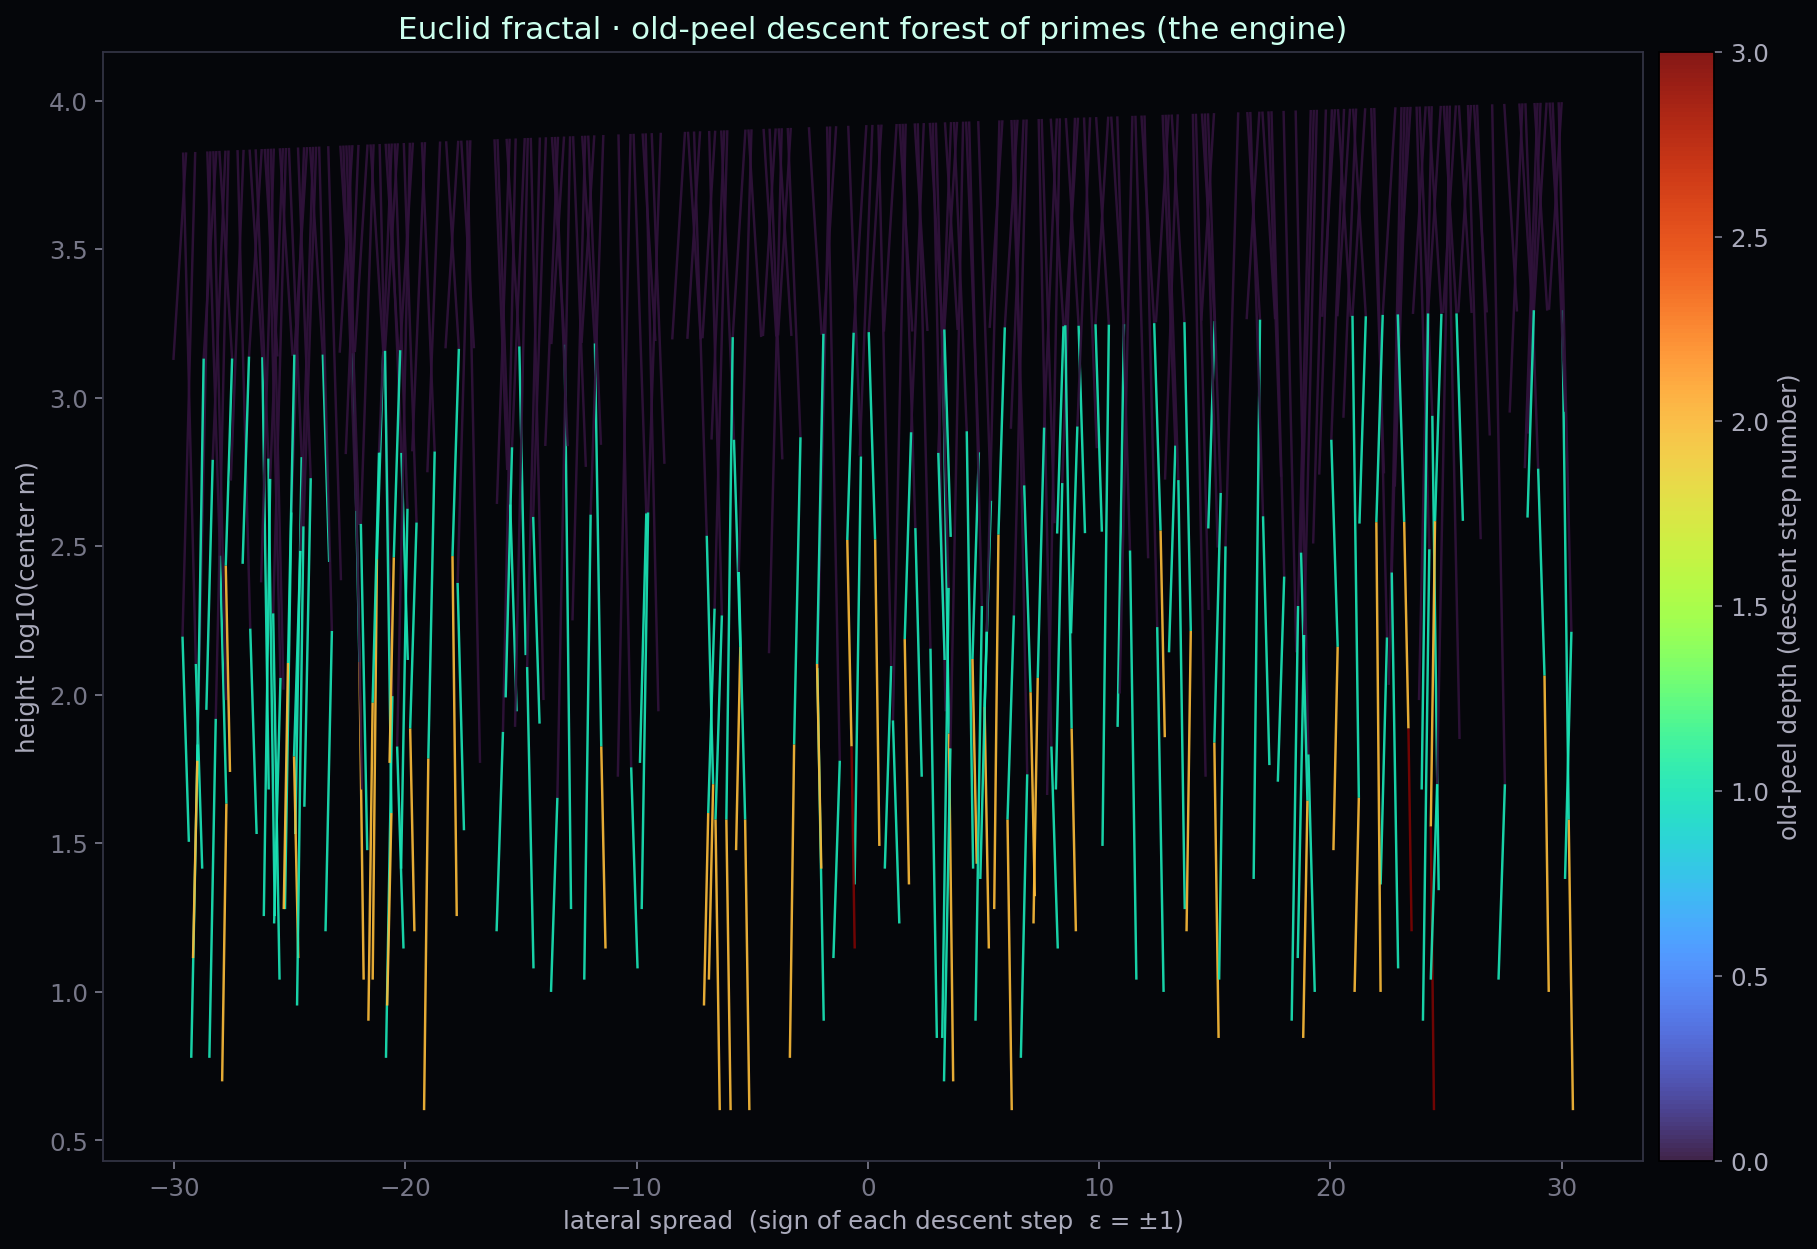
\includegraphics[width=\linewidth]{figures/1_old_peel_tree.png}
  \caption{Old-peel-лес спуска простых --- сам двигатель, запущенный рекурсивно
  из ряда крупных центров.}
  \label{fig:old-peel-tree}
\end{figure}

\emph{Алгоритм генерации (рис.~\ref{fig:old-peel-tree}).} Источник:
\srcpath{tools/fractal/euclid\_fractal.py::old\_peel\_tree}. Фиксируем $A=200$ и
просеиваем все простые до $4A^2$; пул пойманных простых --- простые $p$ с
$3<p\le A$. Разместим горизонтальный ряд из $460$ корней с абсциссами $x$,
равномерно распределёнными по $[-30,30]$; $i$-й корень несёт центр
$n=\lfloor A^2/6\rfloor+7i$. Из каждого корня запускается рекурсивный спуск
$\mathrm{peel}(n,\varepsilon,d,x)$ для обоих знаков $\varepsilon=\pm1$: он
останавливается при глубине $d>7$ или $n<2$; требует, чтобы сторона
$a=6n+\varepsilon$ была простым с $a>A$; берёт противоположную сторону
$6n-\varepsilon$, находит первое простое $p$ из пула, делящее её, образует
частное $q=(6n-\varepsilon)/p$, читает его знак $\delta$ по $q\bmod6$
($\delta=+1$ при $q\equiv1$, $\delta=-1$ при $q\equiv5$, иначе обрыв) и задаёт
дочерний центр $t=(q-\delta)/6$ (обрыв при $t\le0$). Шаг рисует отрезок из
$(x,\ \log_{10}(n+1))$ в $(x+\varepsilon\cdot0.55/(d+1),\ \log_{10}(t+1))$, затем
рекурсивно заходит в $t$ с обоими знаками на глубине $d+1$. Вертикальная ось ---
высота $\log_{10}(\text{центр})$; горизонтальный сдвиг кодирует знак спуска
$\varepsilon$; отрезки окрашены по глубине спуска $d$ (палитра turbo).

\begin{figure}[htbp]
  \centering
  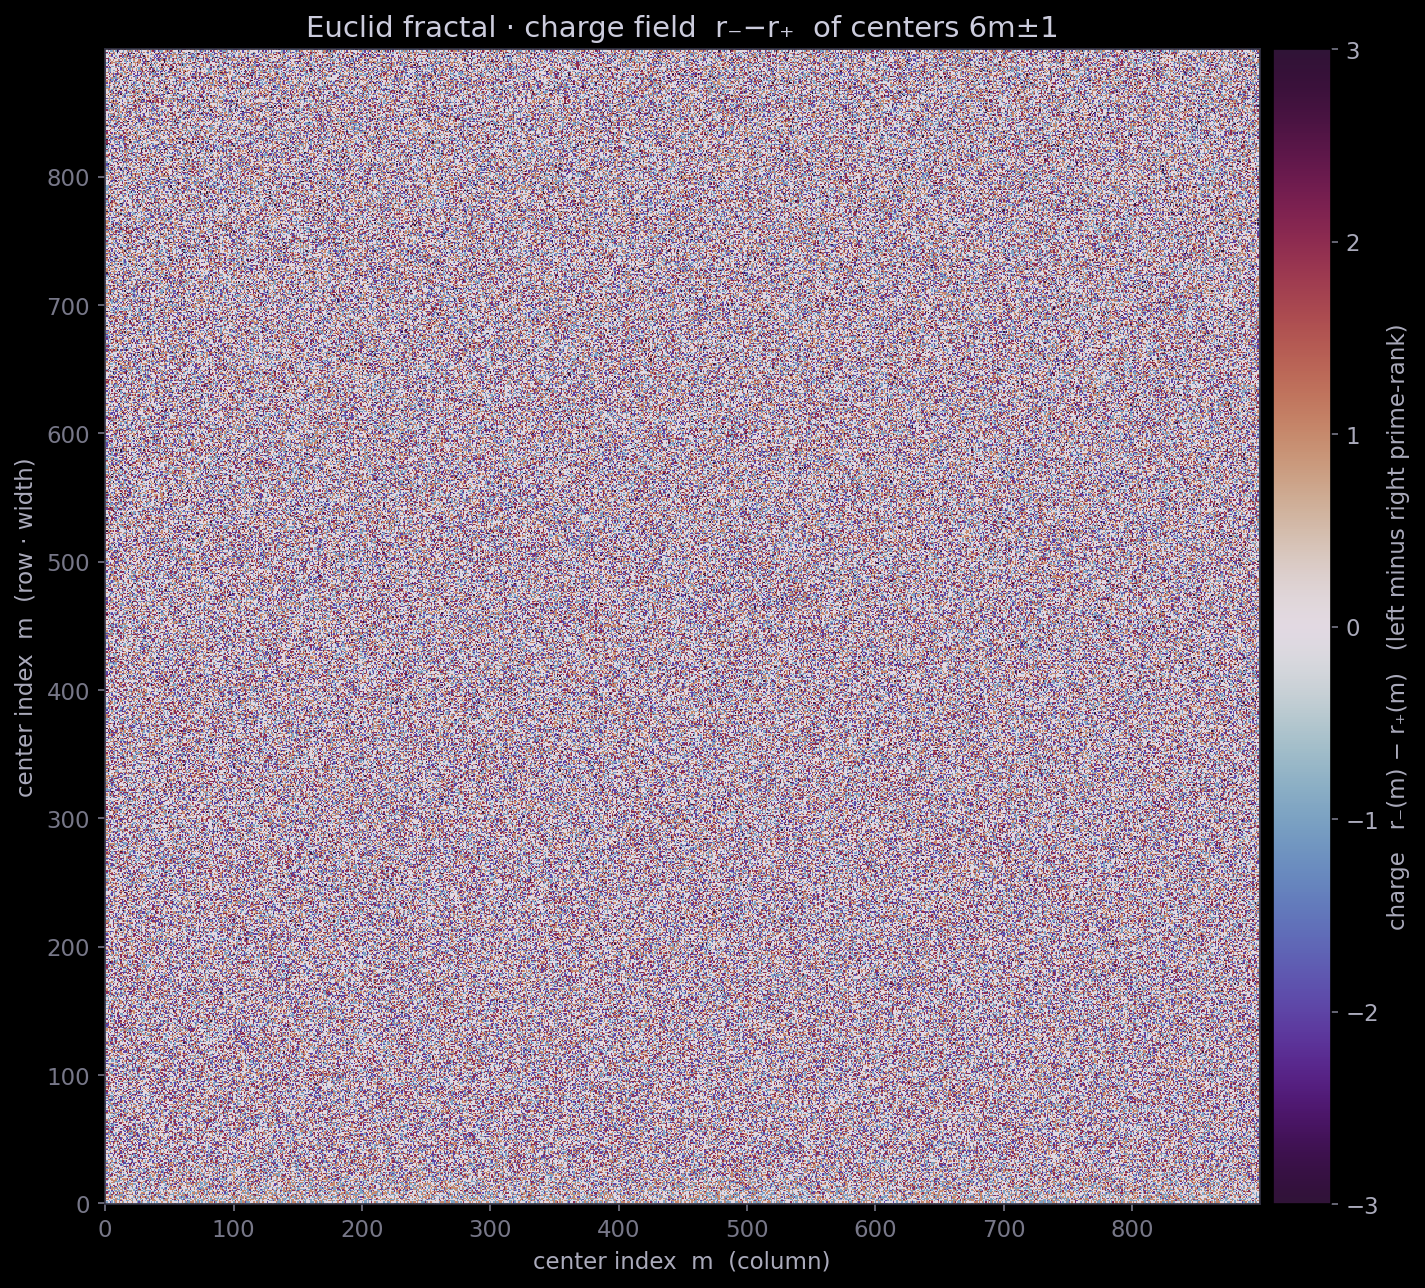
\includegraphics[width=\linewidth]{figures/2_rank_field.png}
  \caption{Поле заряда $r_-(m)-r_+(m)$ центров $6m\pm1$: фрактальная порождающая
  функция простого ранга.}
  \label{fig:rank-field}
\end{figure}

\emph{Алгоритм генерации (рис.~\ref{fig:rank-field}).} Источник:
\srcpath{tools/fractal/euclid\_fractal.py::rank\_field}. Параметры $A=60$, $W=900$;
слой простых --- $\{p:\ A<p\le A^2\}$. Для каждого центрального индекса
$m\in\{0,\dots,W^2-1\}$ считаются два ранга: $r_-(m)$ --- число простых слоя,
делящих нижнюю сторону $6m-1$, и $r_+(m)$ --- верхнюю сторону $6m+1$. Для каждого
$p$ решается сравнение $6m\equiv\pm1\pmod p$ через обратный элемент
$6^{-1}\bmod p$, дающий корень $r\equiv\pm6^{-1}\pmod p$, стартовое смещение
$(r-1)\bmod p$ и единицу, прибавляемую к каждой $p$-й позиции массива $r_\mp$.
Изображается заряд $r_-(m)-r_+(m)$: вектор длины $W^2$ переформатируется в
матрицу $W\times W$ (строка $=\lfloor m/W\rfloor$, столбец $=m\bmod W$) и
рисуется расходящейся палитрой twilight-shifted (противоположные знаки заряда на
двух концах, ноль --- центр), с нижним началом координат.

\begin{figure}[htbp]
  \centering
  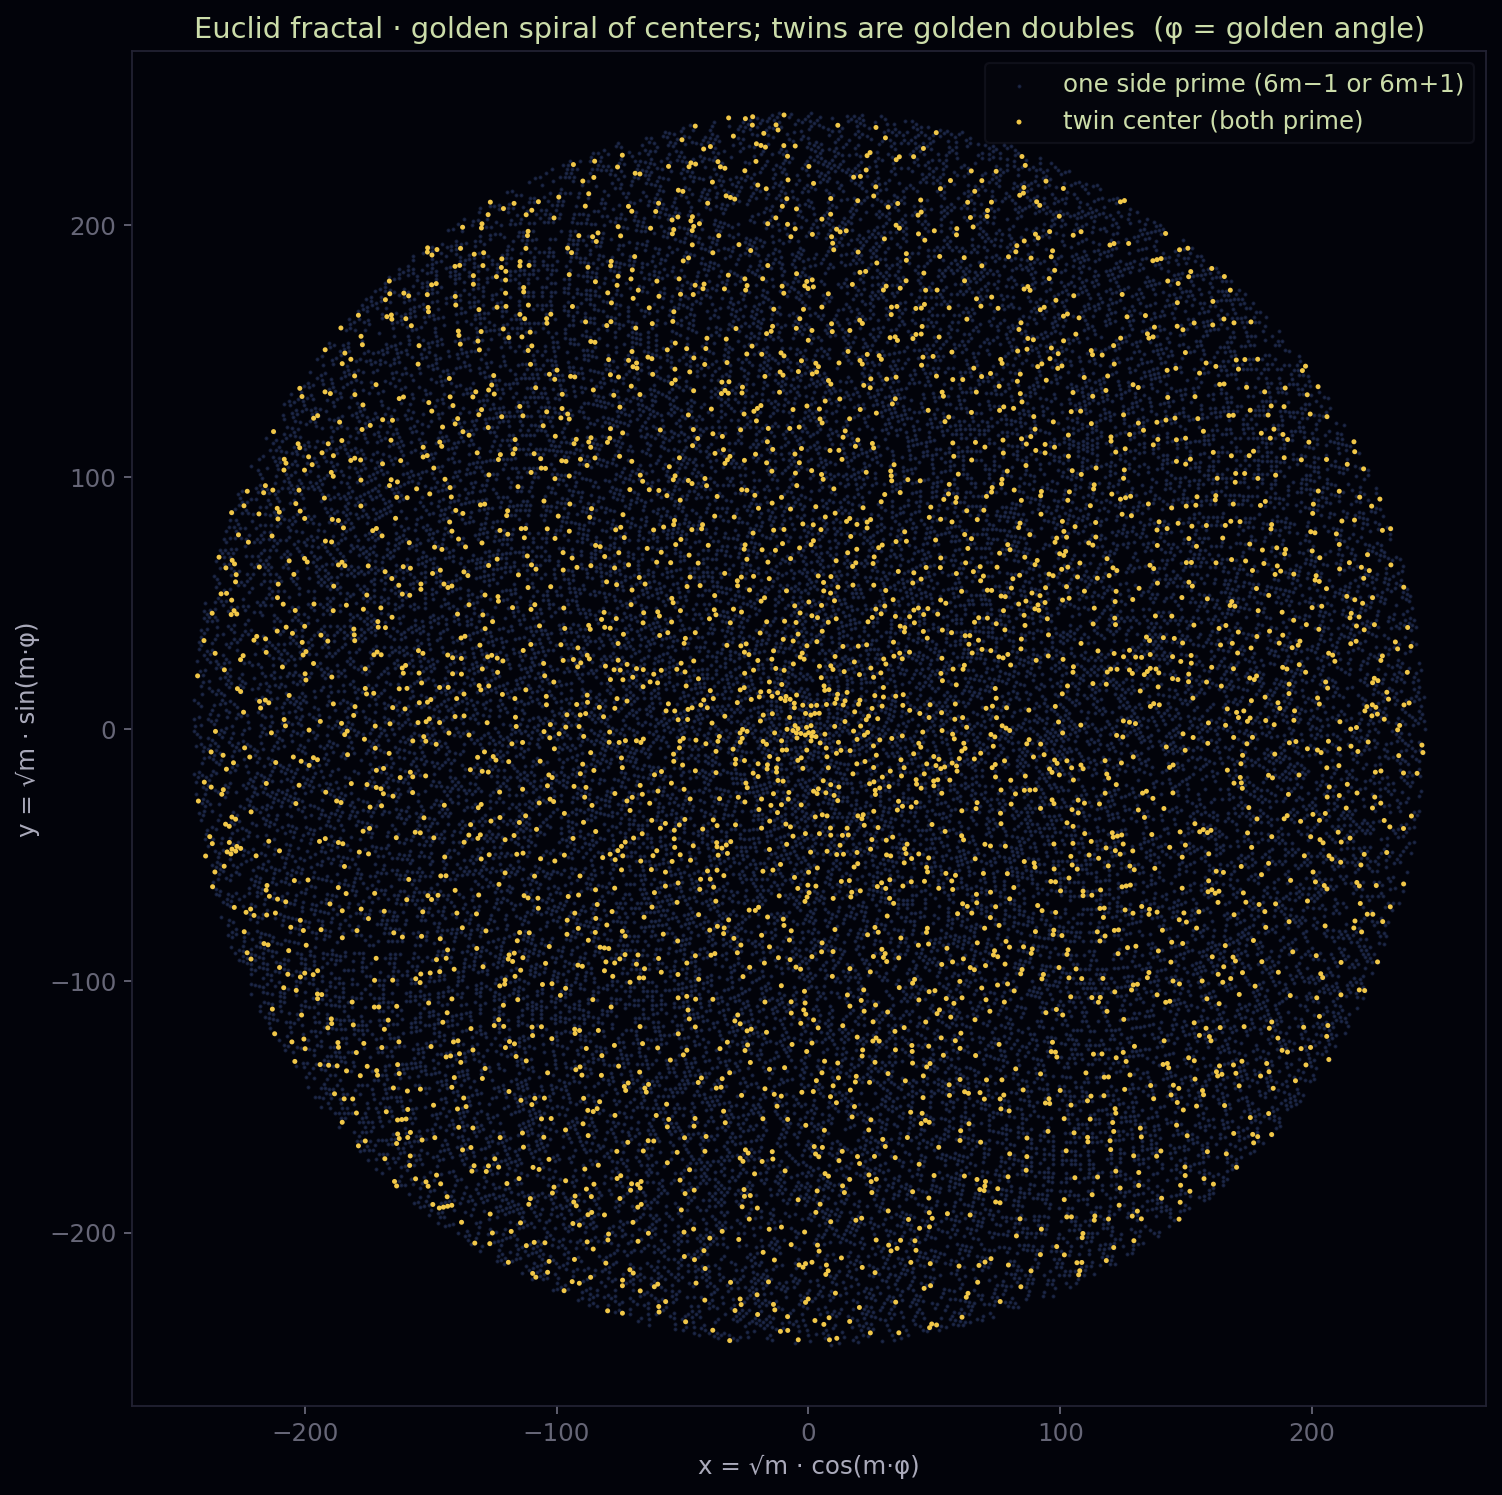
\includegraphics[width=\linewidth]{figures/3_twin_spiral.png}
  \caption{Золотая спираль центров; twin-центры --- золотые двойные точки.}
  \label{fig:twin-spiral}
\end{figure}

\emph{Алгоритм генерации (рис.~\ref{fig:twin-spiral}).} Источник:
\srcpath{tools/fractal/euclid\_fractal.py::twin\_spiral}. Для каждого центра
$m=1,\dots,M-1$ (по умолчанию $M=60000$) точка ставится по золотой спирали
\begin{equation}\label{eq:golden-spiral}
  x=\sqrt{m}\,\cos(m\varphi),\qquad
  y=\sqrt{m}\,\sin(m\varphi),\qquad
  \varphi=\pi(3-\sqrt5),
\end{equation}
где $\varphi$ --- золотой угол. Центр помечается как одна из сторон-простое,
если $6m-1$ или $6m+1$ просто (тускло-синие точки), и как twin-центр, если
просты обе стороны $6m\pm1$ (крупные золотые точки). Радиус $\sqrt m$ даёт
равномерную плотность по площади; цвет постоянен для каждого класса.

\begin{figure}[htbp]
  \centering
  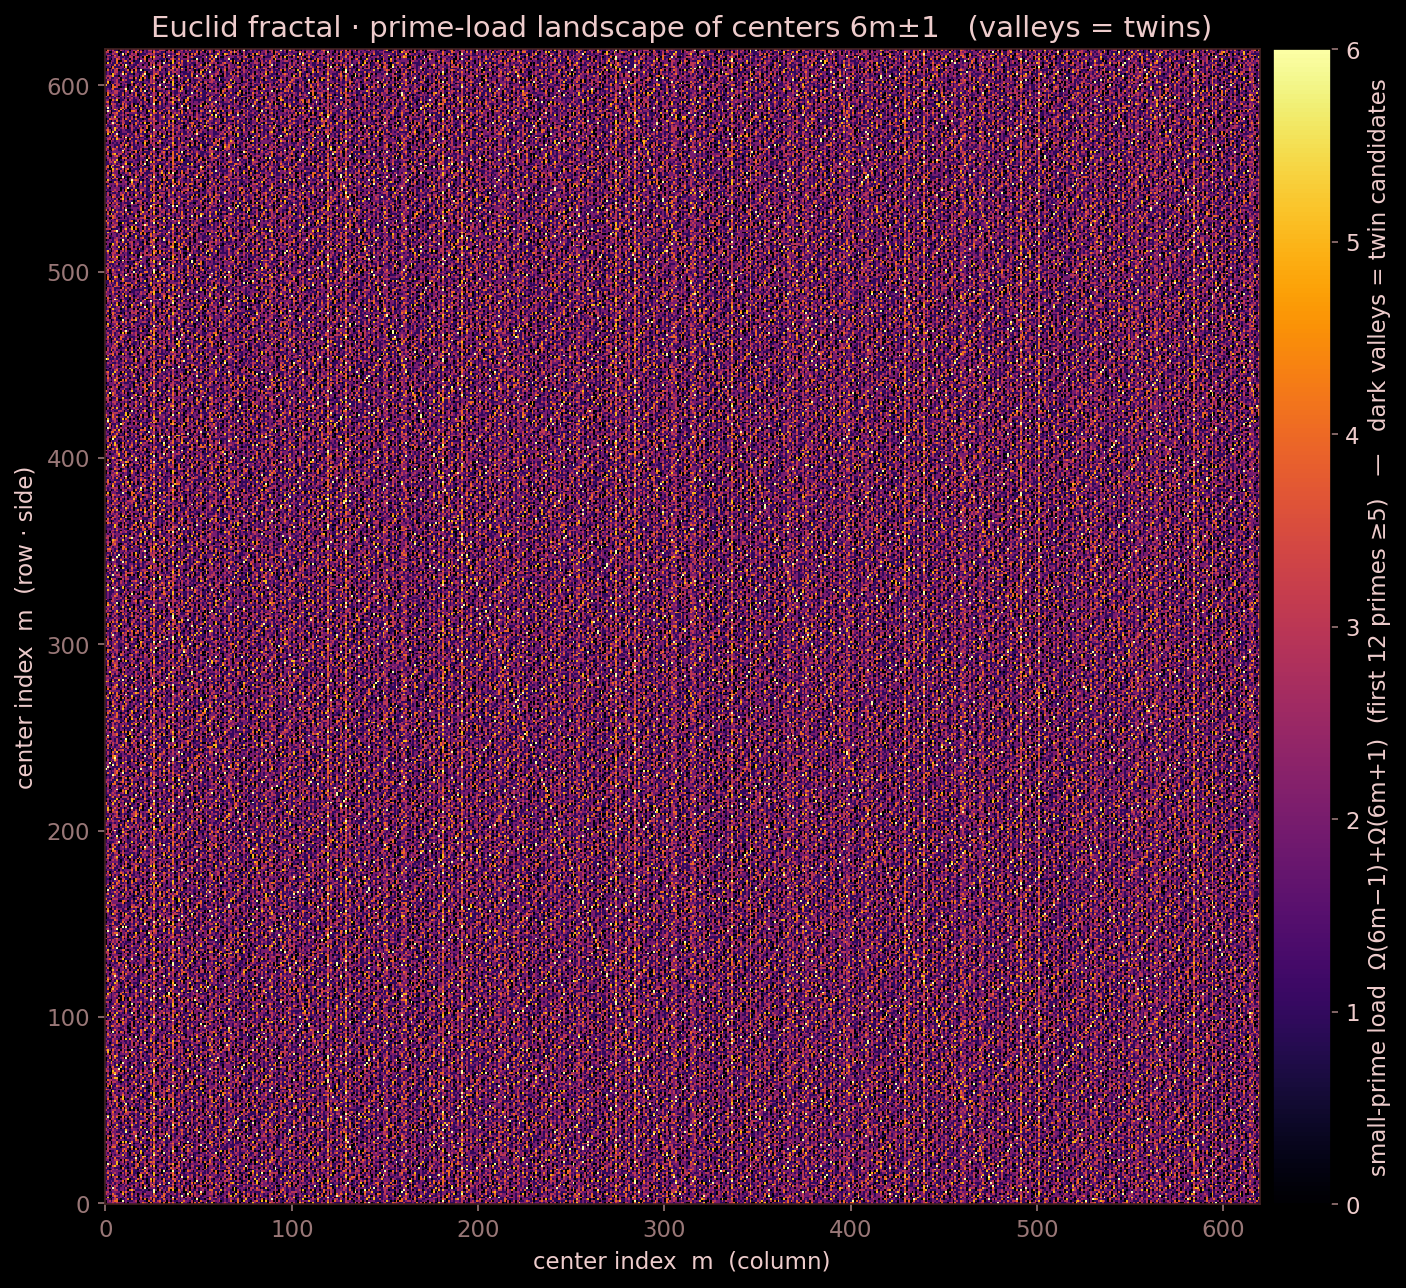
\includegraphics[width=\linewidth]{figures/4_descent_landscape.png}
  \caption{Ландшафт простой нагрузки центров $6m\pm1$; тёмные долины ---
  кандидаты в близнецы.}
  \label{fig:descent-landscape}
\end{figure}

\emph{Алгоритм генерации (рис.~\ref{fig:descent-landscape}).} Источник:
\srcpath{tools/fractal/euclid\_fractal.py::descent\_landscape}. Для каждого центра
$m=0,1,\dots,S^2-1$, разложенного на растр $S\times S$ ($S=620$, построчно по
$m$), вычисляется малопростая нагрузка
\begin{equation}\label{eq:small-prime-load}
  L(m)\;=\;\Omega_B(6m-1)+\Omega_B(6m+1),
\end{equation}
где $\Omega_B(x)$ --- число простых делителей $x$, считаемых с кратностью и
ограниченных первыми $B=12$ простыми $\ge5$ (то есть $5,7,11,\dots,41$). Цвет
ячейки задаётся значением $L(m)$ (палитра inferno, отсечка по 99-му
перцентилю). Центры-близнецы --- где обе стороны $6m\pm1$ просты --- имеют
$L(m)=0$ и образуют тёмные долины; самоподобный рельеф есть
китайско-остаточная периодичность малых простых.

\begin{figure}[htbp]
  \centering
  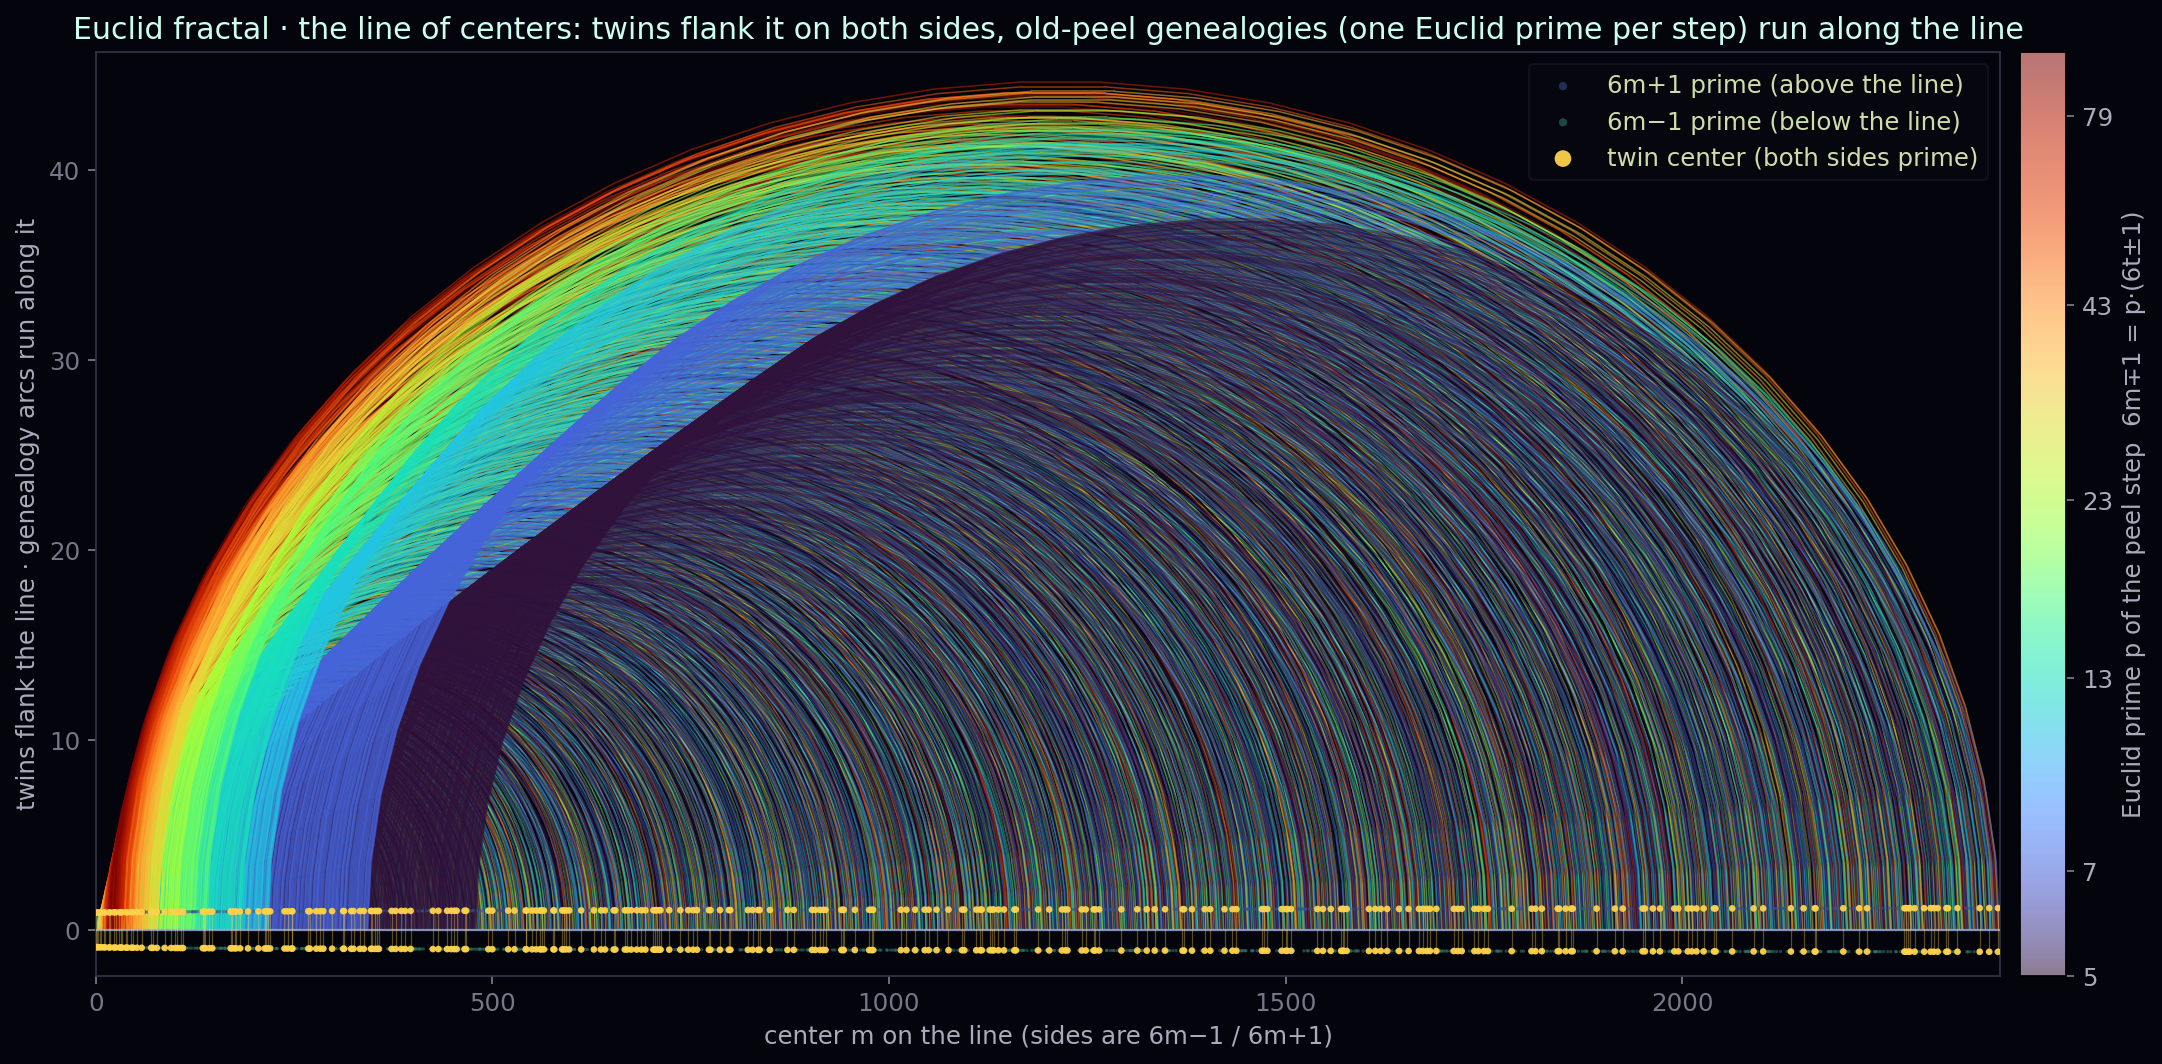
\includegraphics[width=\linewidth]{figures/5_twin_line_genealogy.png}
  \caption{Линия центров: близнецы обрамляют её с двух сторон, old-peel-
  генеалогии (одно евклидово простое на шаг) идут вдоль неё.}
  \label{fig:twin-line-genealogy}
\end{figure}

\emph{Алгоритм генерации (рис.~\ref{fig:twin-line-genealogy}).} Источник:
\srcpath{tools/fractal/euclid\_fractal.py::twin\_line\_genealogy}. Центры
$m=1,\dots,M$ ($M=2400$) откладываются вдоль горизонтальной оси $y=0$. Сторона
$6m+1$ отмечается точкой \emph{над} линией на высоте
$\mathrm{wing}(m)=0.9+0.25\sqrt{m/M}$, сторона $6m-1$ --- симметричной точкой
под линией, когда соответствующее число просто (решето до $6M+2$). Twin-центр
(обе стороны просты) отмечается золотой вертикалью
$[-\mathrm{wing},\,+\mathrm{wing}]$ с точками на концах. Вдоль линии для каждого
$m$ вычисляется old-peel-шаг: если $6m\mp1=p\,(6t\pm1)$ с простым свидетелем
Евклида $p\in[5,97]$, рисуется полуокружностная дуга $m\to t$ высотой
$h=0.06\,|m-t|^{0.85}+0.4$ (36 точек,
$x=\tfrac{m+t}{2}+\tfrac{|m-t|}{2}\cos\theta$, $y=h\sin\theta$,
$\theta\in[0,\pi]$), окрашенная по $\log p$ (палитра turbo). Twin-центры живут
\emph{вне} линии, генеалогия --- \emph{на} ней.

\begin{figure}[htbp]
  \centering
  \includegraphics[width=\linewidth]{figures/6_genealogy_ornament.png}
  \caption{Генеалогический орнамент: полный old-peel-спуск каждого центра,
  сплетённый хордами на окружности центров.}
  \label{fig:genealogy-ornament}
\end{figure}

\emph{Алгоритм генерации (рис.~\ref{fig:genealogy-ornament}).} Источник:
\srcpath{tools/fractal/euclid\_fractal.py::genealogy\_ornament} ($M=4200$,
$\mathrm{PMAX}=97$, $\mathrm{DEPTH}=10$). Центры $1,\dots,M$ сидят на единичной
окружности под углом $2\pi m/M$. Для каждого центра полная old-peel-генеалогия
$m\to t_1\to t_2\to\cdots$ (до глубины $10$) строится шагом
$6k\mp1=p\,(6t\pm1)$: каждый шаг --- хорда Безье с контрольной точкой
$\tfrac12(P_a+P_b)\cdot(1-0.92\min(2\Delta\theta,1))$, где
$\Delta\theta=|a-b|/M$ (длинные хорды ныряют глубже к центру); цвет по
$\log p$ (turbo). Twin-центры (пустая генеалогия) сидят на ободе золотыми
точками.

Два оставшихся рисунка --- концептуальные: они помещают \emph{реальную}
генеалогию в космологическую картину. Подчеркнём честную границу в точности,
как в коде: строго доказаны здесь лишь необратимость времени и кривизна
пространства (невозможность двигателя из \cref{sec:engine}); прочтение
картинок как физики --- перевод, а не теорема.

\begin{figure}[htbp]
  \centering
  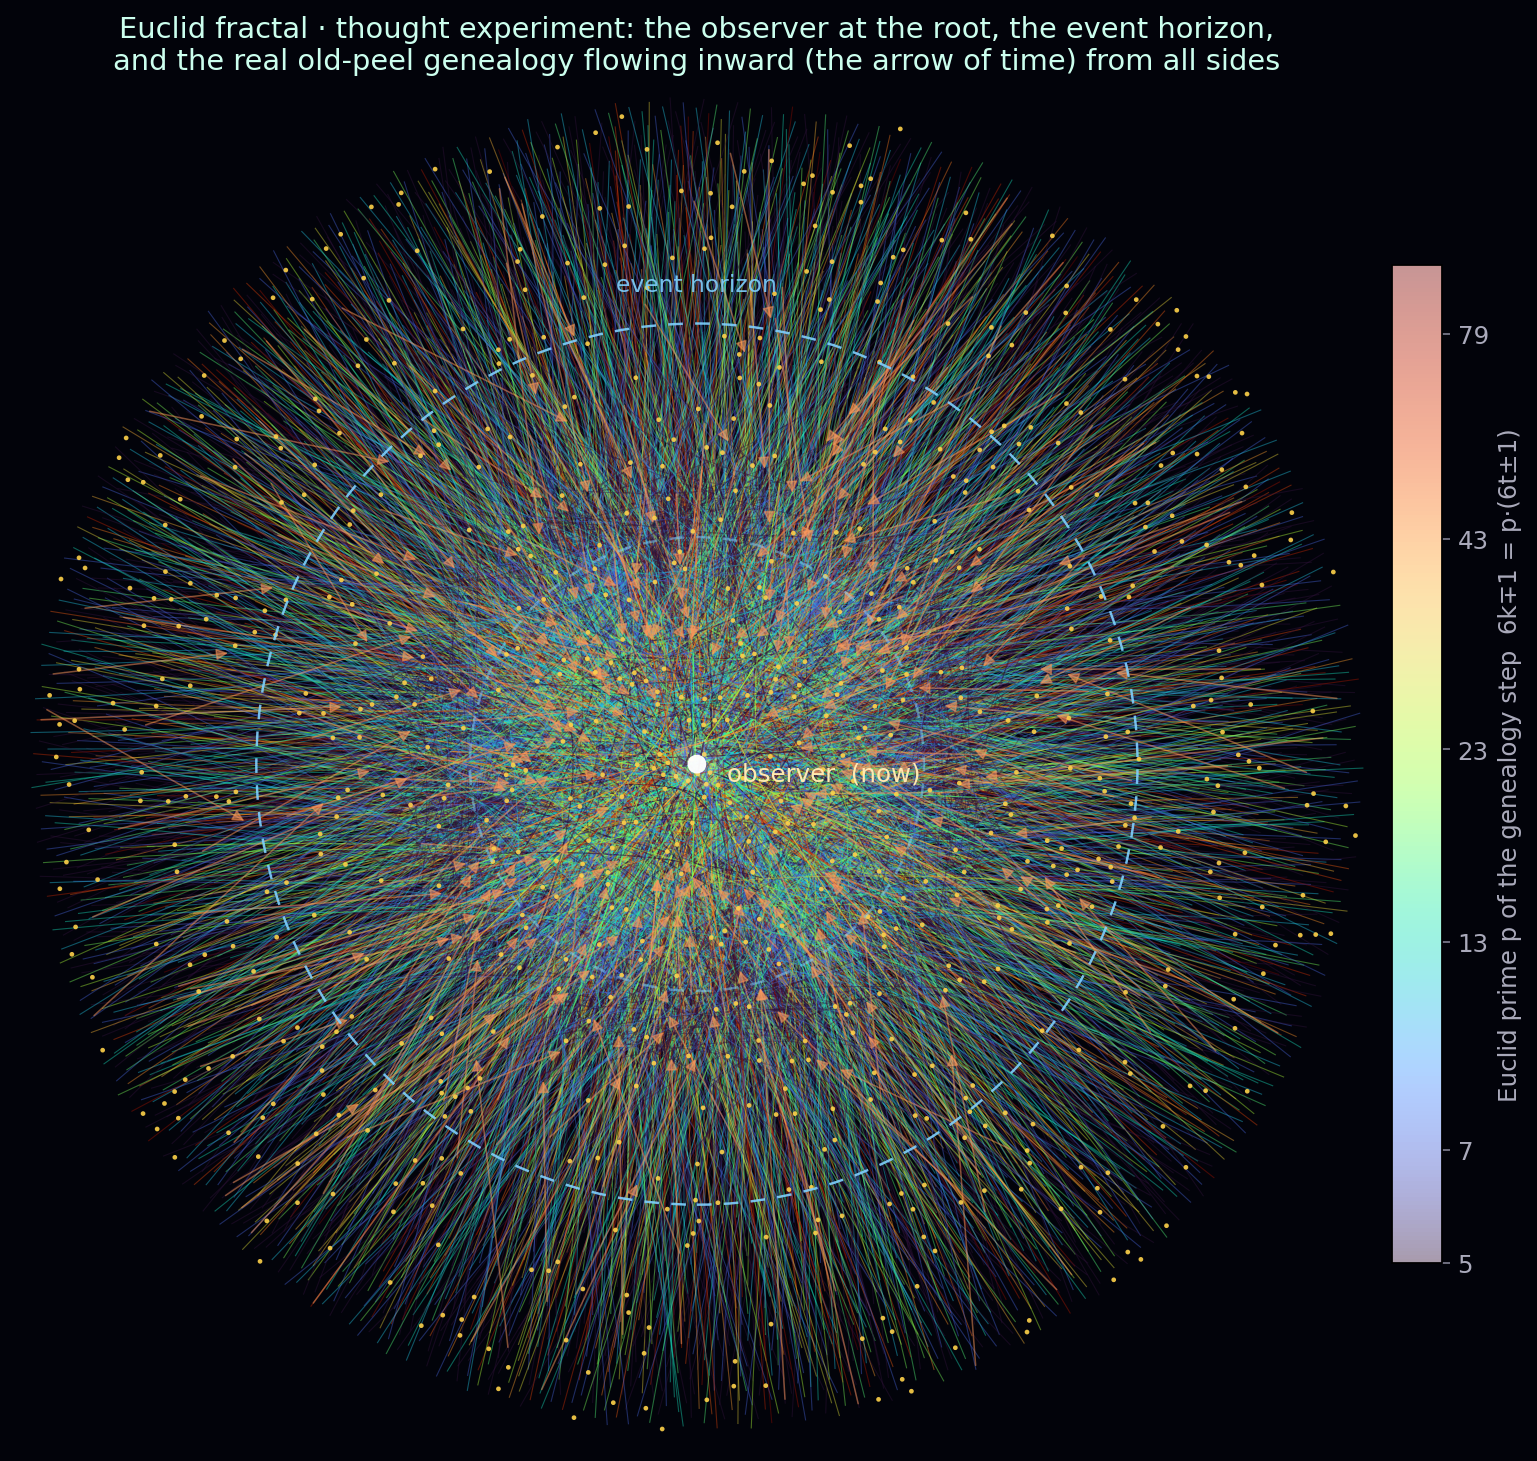
\includegraphics[width=\linewidth]{figures/7_observer_horizon.png}
  \caption{Мысленный эксперимент: наблюдатель у корня, горизонт событий и
  реальная old-peel-генеалогия, текущая внутрь (стрела времени).}
  \label{fig:observer-horizon}
\end{figure}

\emph{Алгоритм генерации (рис.~\ref{fig:observer-horizon}).} Источник:
\srcpath{tools/fractal/euclid\_cosmology.py::observer\_horizon} ($M=9000$,
$\mathrm{PMAX}=97$, $\mathrm{DEPTH}=9$). Центр $k$ размещается на золотой спирали
по радиусу-высоте $r=\sqrt{k/M}$, угол $k\varphi$ ($\varphi$ --- золотой угол):
малые $k$ у центра (наблюдатель), большие --- на периферии. Полная
old-peel-генеалогия каждого центра строится шагом $6k\mp1=p\,(6t\pm1)$
(наименьшее простое-делитель $p\in[5,97]$ композитной стороны, $t<k$),
итерируемым до глубины $9$. Каждый шаг $k\to t$ рисуется квадратичной кривой
Безье с контрольной точкой $\tfrac12(P_k+P_t)\cdot0.72$, подтянутой к началу
(дуга ныряет внутрь); цвет по $\log p$ (палитра turbo). Оранжевые стрелки
ставятся на реальных первых шагах с $r>0.30$ и указывают от $k$ к $t$ (внутрь).
Пунктирные окружности радиусов $0.66$ и $0.34$ --- горизонт событий; золотые
точки --- twin-центры.

\begin{figure}[htbp]
  \centering
  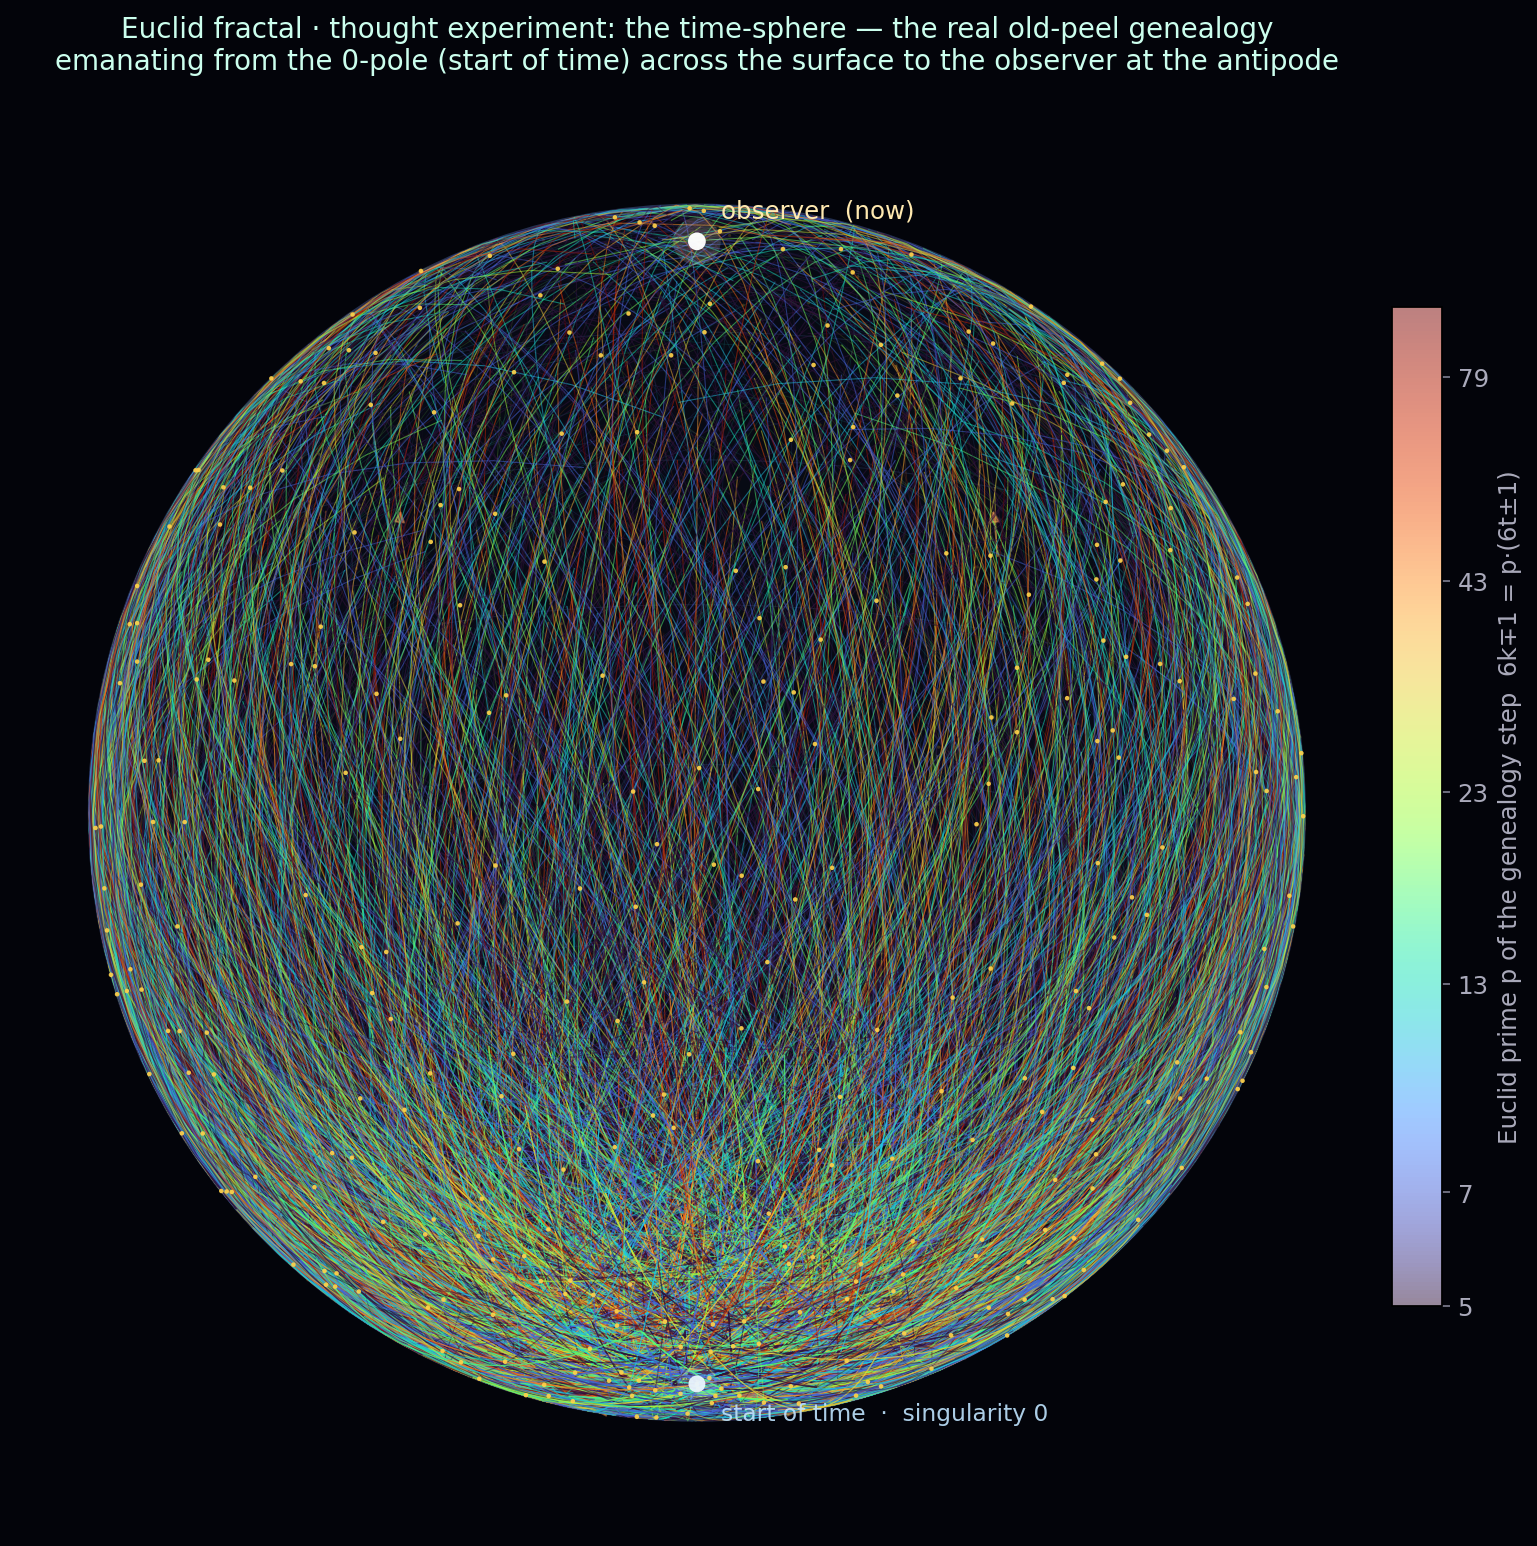
\includegraphics[width=\linewidth]{figures/8_time_sphere.png}
  \caption{Мысленный эксперимент: сфера времени --- реальная
  old-peel-генеалогия, исходящая из полюса-$0$ (старт времени) к наблюдателю в
  антиподе.}
  \label{fig:time-sphere}
\end{figure}

\emph{Алгоритм генерации (рис.~\ref{fig:time-sphere}).} Источник:
\srcpath{tools/fractal/euclid\_cosmology.py::time\_sphere} ($M=7000$,
$\mathrm{PMAX}=97$, $\mathrm{DEPTH}=9$). Центр $k$ отображается в единичный
вектор на сфере: высота $z=-1+2(k-1)/(M-1)$ (так $k=1$ --- в полюсе-$0$,
$z=-1$; $k=M$ --- в полюсе-наблюдателе, $z=+1$), долгота $k\varphi$ по золотому
углу, $\rho=\sqrt{1-z^2}$. Полная old-peel-генеалогия $6k\mp1=p\,(6t\pm1)$
(глубина $9$) рисуется дугами больших кругов (сферический slerp между $V_k$ и
$V_t$); дуги передней полусферы яркие, задней --- тусклые; цвет по $\log p$
(turbo). Проекция --- поворот вокруг оси $x$ на $20^\circ$. Оранжевые стрелки
на меридианах указывают генеративное направление времени от полюса-$0$ к
полюсу-наблюдателю; золотые точки --- twin-центры; два полюса подписаны как
«наблюдатель (сейчас)» и «старт времени $\cdot$ сингулярность $0$».


\bibliographystyle{plain}
\bibliography{refs}

\end{document}
